\documentclass[11pt,a4paper]{report}
\usepackage{epsfig,colordvi,latexsym}
\usepackage{amsmath}
\usepackage{amsfonts}
\usepackage{amssymb}
\usepackage{graphicx}
\usepackage{color}
\usepackage{tikz}  %  for VMCON flowchart in Appendix A
\usepackage{url}
\usepackage{hyperref}
\usepackage{framed}

\pretolerance=10000
\topmargin=0mm
\headheight=0mm
\headsep=8mm
\textwidth=170mm
\textheight=240mm
\footskip=10mm
\oddsidemargin=0mm
\evensidemargin=-12mm
\parskip=2mm
\parindent=0mm

\setcounter{secnumdepth}{3}
\newcommand{\indat}{\mbox{\texttt{IN.DAT}}}
\newcommand{\mfile}{\mbox{\texttt{MFILE.DAT}}}
\newcommand{\outdat}{\mbox{\texttt{OUT.DAT}}}
\newcommand{\plotdat}{\mbox{\texttt{PLOT.DAT}}}
\newcommand{\process}{\mbox{\texttt{PROCESS}}}
\newcommand{\vmcon}{\mbox{\texttt{VMCON}}}
\renewcommand{\vec}[1]{\boldsymbol{#1}}

%%%%%%%%%%%%%%%%%%%%%%%%%%%%%%%%%%%%%%%%%%%%%%%
% Add here the date of the latest change and the code revision number
\newcommand{\version}{
2015-01-29
\hfill
Revision: 382
}
%%%%%%%%%%%%%%%%%%%%%%%%%%%%%%%%%%%%%%%%%%%%%%%

\newcommand{\setheader}[1]
 {\markright{\rlap{\lower0.8ex\hbox to\textwidth{\hrulefill}}{\bf#1}}}
\newcommand{\mychapter}[1]{\small\normalsize
 \setcounter{footnote}{0}
 \chapter{#1}
 \pagestyle{myheadings}
 \setheader{Chapter \thechapter\hspace{0.8em}#1}}
\newcommand{\myappendix}[1]{\small\normalsize
 \setcounter{footnote}{0}
 \chapter{#1}
 \pagestyle{myheadings}
 \setheader{Appendix \thechapter\hspace{0.8em}#1}}

\begin{document}

\footnotesize
\hfill T\&M/PKNIGHT/PROCESS/MANUAL

\vspace*{4cm}
\begin{center}
\Huge A User Guide\\ to the \\ PROCESS Systems Code\\
~\\ \LARGE P.\ J.\ Knight\\
~\\ \Large Culham Centre for Fusion Energy\\
Culham Science Centre, Abingdon, Oxon, OX14 3DB, UK
\end{center}

\vfill
\footnotesize
\version
\normalsize

\tableofcontents

\listoffigures

\listoftables

%%%%%%%%%%%%%%%%%%%%%%%%%%%%%%%%%%%%%%%%%%%%%%%%%%%%%%%%%%%%%%%%%%%%%%%%%%
% To do list:
%  (apart from bringing it in line with the F90 code, of course...)
%  scaling law references into table
%  IFE model; expand details about build, materials
%  check and expand references
%  show buildings calculations
%  iavail usage
%  tratio
%  density limit refs
%  check PF coil location
%  add descriptions of other switches
%  
%  
%  
%  
%  
%  
%%%%%%%%%%%%%%%%%%%%%%%%%%%%%%%%%%%%%%%%%%%%%%%%%%%%%%%%%%%%%%%%%%%%%%%%%%

\mychapter{Introduction}
\label{chap:intro}

\section{Rationale}

During the course of studies into a proposed fusion power plant, there may be
times when questions of the following type arise:
\begin{quote}
Are the machine's physics and engineering parameters consistent with one
another?

Which machine of a given size and shape produces the cheapest electricity?

What is the effect of a more optimistic limit on the maximum plasma density on
the amount of auxiliary power required?
\end{quote}

Questions such as these are extremely difficult to answer, since the large
number of parameters involved are highly dependent on one another.
Fortunately, computer programs have been written to address these issues, and
\process\ is one of them.

Suppose that an outline power plant design calls for a machine with a given
size and shape, which will produce a certain net electric power.  There may be
a vast number of different conceptual machines that satisfy the problem as
stated so far, and \process\ can be used in ``non-optimisation'' mode to find
one of these whose physics and engineering parameters are
self-consistent. However, the machine found by \process\ in this manner may
not be possible to build in practice --- the coils may be overstressed, for
instance, or the plasma pressure may exceed the maximum possible
value. \process\ contains a large number of constraints to prevent the code
from finding a machine with such problems, and running the code in so-called
``optimisation'' mode forces these constraints to be met. The number of
possible conceptual machines is thus considerably reduced, and optimisation of
the parameters with respect to (say) the cost of electricity will reduce this
number to a minimum (possibly one).

Formally then, \process\ is a systems code that calculates in a
self-consistent manner the parameters of a fusion power plant with a specified
performance, ensuring that its operating limits are not violated, and with the
option to optimise a given function of these parameters.

\section{History}

\process\ is derived from several earlier systems codes, but is largely based
on the TETRA (Tokamak Engineering Test Reactor Analysis) code~\cite{tetra} and
its descendant STORAC (Spherical TOrus Reactor Analysis Code)~\cite{storac},
which includes routines relevant to the spherical tokamak class of
machines. These codes, and much of the original version of \process\ itself,
were written by personnel at Oak Ridge National Laboratory in Tennessee, USA,
with contributions from a number of other laboratories in the USA\@. In
addition, many of the mathematical routines have been taken from a number of
different well-established source libraries.

A great deal of effort was expended at Culham on the code's arrival from ORNL in the early
1990s to upgrade and extend the code, including the addition of machines based on the stellerator, reversed field pinch and inertial confinement concepts.

\process\ is being developed actively. This User Guide is updated in parallel with the 
code itself to ensure that the documentation remains consistent with
the latest version of the code. It is to be hoped that it will be of
assistance not only to users of \process, but to anyone using  \process\ outputs or models based on them.

%\section{Layout of the User Guide}

%Chapter~\ref{chap:overview} provides an overview of the program, and outlines
%the numerical and programming concepts involved. Chapter~\ref{chap:models}
%describes the physics, engineering and economic models that are used within
%the code, and lists the switches available allowing the user to customise the
%models' details to achieve the desired simulation. Chapter~\ref{chap:run}
%describes how to run the program from scratch, and provides a number of hints
%and suggestions for the user to bear in mind to help the code find a feasible
%machine. Chapter~\ref{chap:modify} shows how to modify the code in specific
%ways, for example how to add extra constraints and variables to the code. A
%useful set of utility programs is introduced in Chapter~\ref{chap:utilities},
%and some code management tools are described in
%Chapter~\ref{chap:codetools}. Finally, the Appendices give detailed
%information about the optimisation method, and example input files for \process\
%in non-optimisation and optimisation modes.

\section{Sources of information}

The output file OUT.DAT contains details of all the constraints and iteration variables selected, the input and output parameters, and which models have been chosen. It is essential to study the full output before using the results in any way.

Details of the physics, engineering and cost models are being published:

~\cite{kovari_physics}: M. Kovari et al., PROCESS: a systems code for fusion power plants - Part 1: Physics

~\cite{kovari_eng}: M. Kovari et al., PROCESS: a systems code for fusion power plants - Part 2: Engineering, in preparation

~\cite{kovari_cost}: M. Kovari et al., The cost of a fusion power plant: extrapolation from ITER, in preparation

To view sample input and output files and a description of the variables, or to report bugs, request improvements, propose new models, or contact the \process\ developers, please visit

\textcolor{blue}{\href{http://www.ccfe.ac.uk/powerplants.aspx}{ccfe.ac.uk/powerplants.aspx}}.

  %  Introduction
\mychapter{Program Overview --- The Fundamental Concepts}
\label{chap:overview}

Fusion power plants are complex systems consisting of many non-linear
interactions. One method that can be used to model this kind of system is to
iterate a number of free parameters (the so-called \textit{iteration
  variables} --- see Section~\ref{sec:itvars}) in a controlled way so as to
find a self-consistent set of device parameters that satisfy all of the
system's \textit{constraint equations} --- see
Section~\ref{sec:constraints}. \process\ is organised in a standard equation
solver format to enable this task to be performed efficiently. The physics and
engineering routines together serve as a \textit{function evaluator},
providing the information used in the solution of the constraints. The
numerical modules present in \process\ perform the iteration required, and
also incorporate the option to maximise or minimise a given \textit{figure of
  merit} -- see Section~\ref{sec:foms}.

\section{Equation Solvers}

\process\ contains two non-linear equation solver packages, which reflect the
two major modes of operation available. Each of these has its own uses, as is
now discussed.

\subsection{Non-optimisation mode}

The first of the two equation solvers present in \process\ is the
non-optimisation package HYBRD~\cite{hybrd_anl,hybrd}. Formally, HYBRD
finds a zero of a system of $N$ non-linear functions in $N$ variables. This
means simply that $N$ variables (power plant parameters) are iterated by
\process\ in such a way as to solve a set of $N$ equations (physics or
engineering laws), i.e.\ a set of self-consistent power plant parameters is
found. This is useful for performing benchmark comparisons, when the device
size is kept fixed, and one only wishes to find calculated stresses, beta
values, fusion powers, etc. A flow diagram of \process\ in non-optimisation
mode is shown in Figure~\ref{fig:flow_hybrd}.

% Flow diagram for HYBRD run

\setlength{\unitlength}{1mm}

\begin{figure}[tbph]
\begin{center}

\begin{picture}(140.0,140.0)(0.0,60.0)

\put(50.0,197.0){\makebox(0,0){initialise variables}}
\put(50.0,185.0){\makebox(0,0){input from file}}
\put(50.0,173.0){\makebox(0,0){define free parameters}}
\put(50.0,161.0){\makebox(0,0){define rules}}
\put(50.0,155.0){\makebox(0,0){to be obeyed}}
\put(50.0,137.0){\makebox(0,0){evaluate physics, engineering}}
\put(50.0,131.0){\makebox(0,0){and cost functions}}
\put(50.0,119.0){\makebox(0,0){apply consistency equations}}
\put(50.0,77.0){\makebox(0,0){write output}}
\put(110.0,125.0){\makebox(0,0){iterate}}
\put(110.0,119.0){\makebox(0,0){free parameters}}

\thicklines

\put(30.0,194.0){\framebox(40.0,6.0){}}
\put(34.0,182.0){\framebox(32.0,6.0){}}
\put(28.0,170.0){\framebox(44.0,6.0){}}
\put(34.0,152.0){\framebox(32.0,12.0){}}
\put(22.0,128.0){\framebox(56.0,12.0){}}
\put(22.0,116.0){\framebox(56.0,6.0){}}
\put(34.0,74.0){\framebox(32.0,6.0){}}
\put(94.0,116.0){\framebox(32.0,12.0){}}

\put(50.0,98.0){\makebox(0,0){self-consistent?}}
\put(50.0,86.0){\line(-2,1){24.0}}
\put(26.0,98.0){\line(2,1){24.0}}
\put(50.0,110.0){\line(2,-1){24.0}}
\put(74.0,98.0){\line(-2,-1){24.0}}

\put(44.0,82.0){yes}
\put(78.0,100.0){no}

\put(50.0,194.0){\vector(0,-1){6.0}}
\put(50.0,182.0){\vector(0,-1){6.0}}
\put(50.0,170.0){\vector(0,-1){6.0}}
\put(50.0,152.0){\vector(0,-1){12.0}}
\put(50.0,128.0){\vector(0,-1){6.0}}
\put(50.0,116.0){\vector(0,-1){6.0}}
\put(50.0,86.0){\vector(0,-1){6.0}}
\put(74.0,98.0){\vector(1,0){18.0}}
\put(110.0,98.0){\vector(0,1){9.0}}
\put(110.0,128.0){\vector(0,1){9.0}}
\put(110.0,146.0){\vector(-1,0){30.0}}

\put(92.0,98.0){\line(1,0){18.0}}
\put(110.0,107.0){\line(0,1){9.0}}
\put(110.0,137.0){\line(0,1){9.0}}
\put(80.0,146.0){\line(-1,0){30.0}}

\thinlines
\end{picture}

\end{center}
\caption[Flow diagram of \process\ in non-optimisation mode]
{\label{fig:flow_hybrd}
  \textit{Flow diagram of \process\ in non-optimisation mode.}
}
\end{figure}

\subsection{Optimisation mode}

%\author{H. Lux}%

Sometimes one wants to find an optimal machine that is both consistent with
the physics and engineering constraints but also minimises or maximises a
certain \textit{figure of merit}. This requires running \process\/ in
optimisation mode. For these applications \process\/ uses the routine \vmcon\/
\cite{vmcon} based on a variable metric method for constrained optimisation by
Powell \cite{Powell1978}. It finds a stationary point of an objective
function/figure of merit consistent with a set of equality and inequality
constraints (c.f. section \ref{sec:GNPP}). It is designed to solve the
necessary but not sufficient conditions of a constrained optimum, hence, the
solution does not have to be a global optimum (c.f. \ref{sec:Lagrange}).

The detailed algorithm is explained in Appendix~\ref{app:Opt} and is based on
the Lagrange method (c.f. section \ref{sec:Lagrange}) that combines both the
objective function and the constraints using Lagrange multipliers. It applies
a sequential quadratic programming approach (c.f. section \ref{sec:SQP}) in
which a series of subproblems is solved that constitute a local quadratic
expansion of the Lagrangian (c.f. section \ref{sec:QSP}). The solution of the
quadratic subproblem is the direction of a line search along which a one
dimensional optimisation is performed (c.f. section
\ref{sec:linesearch}). This line search was introduced by Powell to assure
convergence from bad starting parameters. Within \process\/ we have modified
the line search of the original \vmcon\/ routine to assure convergence, even
for slightly inconsistent input functions.

The algorithm uses a quasi-Newtonian approach which only requires continuous
first derivatives of these functions. While the first derivatives are
evaluated using a finite difference approximation, the second derivatives are
estimated using a variant of the Broyden-Fletcher-Goldfarb-Shanno update
(c.f. section \ref{sec:BFGS}).

The convergence criterium of the solver as well as the detailed interpretation
of the various error codes are explained in section \ref{sec:vmcon}. A flow
diagram of \process\/ in optimisation mode is shown in Figure
\ref{fig:flow_vmcon}.

% Flow diagram for VMCON run

\setlength{\unitlength}{1mm}

\begin{figure}[tbph]
\begin{center}

\begin{picture}(140.0,200.0)

\put(50.0,197.0){\makebox(0,0){initialise variables}}
\put(50.0,185.0){\makebox(0,0){input from file}}
\put(50.0,173.0){\makebox(0,0){define free parameters}}
\put(50.0,161.0){\makebox(0,0){define rules}}
\put(50.0,155.0){\makebox(0,0){to be obeyed}}
\put(50.0,143.0){\makebox(0,0){define performance}}
\put(50.0,137.0){\makebox(0,0){requirements}}
\put(50.0,125.0){\makebox(0,0){define figure-of-merit}}
\put(50.0,107.0){\makebox(0,0){evaluate physics, engineering}}
\put(50.0,101.0){\makebox(0,0){and cost functions}}
\put(50.0,89.0){\makebox(0,0){apply consistency equations}}
\put(50.0,83.0){\makebox(0,0){and limit equations}}
\put(50.0,11.0){\makebox(0,0){write output}}
\put(110.0,92.0){\makebox(0,0){iterate}}
\put(110.0,86.0){\makebox(0,0){free parameters}}

\thicklines

\put(30.0,194.0){\framebox(40.0,6.0){}}
\put(34.0,182.0){\framebox(32.0,6.0){}}
\put(28.0,170.0){\framebox(44.0,6.0){}}
\put(34.0,152.0){\framebox(32.0,12.0){}}
\put(30.0,134.0){\framebox(40.0,12.0){}}
\put(28.0,122.0){\framebox(44.0,6.0){}}
\put(22.0,98.0){\framebox(56.0,12.0){}}
\put(22.0,80.0){\framebox(56.0,12.0){}}
\put(34.0,8.0){\framebox(32.0,6.0){}}
\put(94.0,83.0){\framebox(32.0,12.0){}}

\put(50.0,62.0){\makebox(0,0){self-consistent?}}
\put(50.0,50.0){\line(-2,1){24.0}}
\put(26.0,62.0){\line(2,1){24.0}}
\put(50.0,74.0){\line(2,-1){24.0}}
\put(74.0,62.0){\line(-2,-1){24.0}}

\put(44.0,46.0){yes}
\put(78.0,64.0){no}

\put(50.0,32.0){\makebox(0,0){F-o-M minimised?}}
\put(50.0,20.0){\line(-2,1){24.0}}
\put(26.0,32.0){\line(2,1){24.0}}
\put(50.0,44.0){\line(2,-1){24.0}}
\put(74.0,32.0){\line(-2,-1){24.0}}

\put(44.0,16.0){yes}
\put(78.0,34.0){no}

\put(50.0,194.0){\vector(0,-1){6.0}}
\put(50.0,182.0){\vector(0,-1){6.0}}
\put(50.0,170.0){\vector(0,-1){6.0}}
\put(50.0,152.0){\vector(0,-1){6.0}}
\put(50.0,134.0){\vector(0,-1){6.0}}
\put(50.0,122.0){\vector(0,-1){12.0}}
\put(50.0,98.0){\vector(0,-1){6.0}}
\put(50.0,80.0){\vector(0,-1){6.0}}
\put(50.0,50.0){\vector(0,-1){6.0}}
\put(50.0,20.0){\vector(0,-1){6.0}}
\put(74.0,62.0){\vector(1,0){18.0}}
\put(74.0,32.0){\vector(1,0){18.0}}
\put(110.0,62.0){\vector(0,1){10.5}}
\put(110.0,32.0){\vector(0,1){15.0}}
\put(110.0,95.0){\vector(0,1){10.5}}
\put(110.0,116.0){\vector(-1,0){30.0}}

\put(92.0,62.0){\line(1,0){18.0}}
\put(92.0,32.0){\line(1,0){18.0}}
\put(110.0,47.0){\line(0,1){15.0}}
\put(110.0,72.5){\line(0,1){10.5}}
\put(110.0,105.5){\line(0,1){10.5}}
\put(80.0,116.0){\line(-1,0){30.0}}

\thinlines
\end{picture}

\end{center}
\caption[Flow diagram of \process\ in optimisation mode]
{\label{fig:flow_vmcon} \textit{Conceptual flow diagram of \process\/ in
    optimisation mode. Please note that this is a simplistic interpretation of
    the actual sequence of operations, to outline the difference between
    non-optimisation and optimisation modes. For a more detailed (and
    correct!) \vmcon\ flow diagram, please see Figure~\ref{fig:vmconflow}.}  }
\end{figure}

\subsection{Scans}

It is often useful to be able to scan through a range of values of a given
parameter to see what effect this has on the machine as a whole.  Sensitivity
studies of this kind can be achieved very easily using \process. Scans are
carried out in optimisation mode, whereby the code performs initially a run
using the parameters specified in the input file, and then a series of runs
using the parameters produced at the end of the previous iteration. The value
of the quantity being scanned is specified at every stage --- see
Section~\ref{sec:scans}. This method ensures that a smooth variation in the
machine parameters is achieved.

\section{The Variable Descriptor File}
\label{sec:vardes}

The variable descriptor file \texttt{vardes.html} is an invaluable resource for
the user of \process. It acts as a dictionary / reference manual for the
code's variables, and contains the following information about each:
\begin{itemize}
\item name
\item dimensions (of arrays)
\item default value(s) of those variables that are not initially derived from
  a combination of other values. The default values are mostly set in the
  modules contained within source file \texttt{global\_variables.f90}.
\item description, including physical units if relevant
\item for switches/flags, the meanings of all allowed values
\item iteration variable number, if relevant
\item corresponding constraint equation, if relevant
\end{itemize}
In addition, global code parameters are labelled \texttt{FIX}. These can only
be changed by editing the relevant source file, but this should not be carried
out unless it is absolutely necessary.

All the variables that are shown with a default value are available to be
changed by the user using the input file (Section~\ref{sec:infile}), except
for those which are labelled \texttt{FIX}. Variables not shown with a default
value are calculated by the code from a combination of other parameters, and
so it would be meaningless to initialise them.  Obviously, these variables
cannot be changed using the input file.

The file is generated from specially-formatted comment lines within the source
code (see Section~\ref{sec:autodoc} for more details). Therefore, it is
exceedingly important to keep these comment lines relevant and in sync with
the variables they describe.

\section{Input Parameters}
\label{sec:inpars}

Input parameters make up a large proportion of the variables listed in the
variable descriptor file. They comprise all those variables that, once set in
the initialisation routine or redefined in the input file, do not change
throughout a \process\ run. In fact, only those variables defined as iteration
variables (Section~\ref{sec:itvars}) can change during the course of a run.

\section{Constraint Equations}
\label{sec:constraints}

Any computer program naturally contains myriads of equations. The built-in
equation solvers within \process\ act on a special class, known as
\textit{constraint equations}, all of which are formulated in routine
\texttt{CONSTRAINTS} in source file
\texttt{constraint\_equations.f90}. Table~\ref{tab:eqns} summarises the
constraint equations available in \process. These can be split into two types
--- (1) consistency equations, that enforce consistency between the physics
and engineering parameters, and (2) limit equations, that enforce various
parameters to lie within their allowed limits. The \texttt{neqns} constraint
equations that the user chooses for a given run are activated by including the
equation numbers in the first \texttt{neqns} elements of array \texttt{icc}.

\subsection{Consistency equations}

Consistency equations are usually \textit{equalities}\/ that ensure that the
machine produced by \process\ is self-consistent. This means, therefore, that
many of these constraint equations should \textit{always}\/ be used, namely
equations~1, 2, 10 and 11 (see Table~\ref{tab:eqns}).  Equation~7 should also
be activated if neutral beam injection is used.  The other consistency
equations can be activated if required.

A typical consistency equation ensures that two functions $g$ and $h$ are
equal:
\begin{eqnarray*}
g(x,y,z,\ldots) & = & h(x,y,z,\ldots) \\
c_i & = & 1 - \frac{g}{h}
\end{eqnarray*}
The equation solvers VMCON and HYBRD need the constraint equations $c_i$ to be
given in the form shown, since they adjust the iteration variables so as to
obtain $c_i = 0$, thereby ensuring that $g = h$.

\subsection{Limit equations}

The limit equations are usually \textit{inequalities}\/ that ensure that
various physics or engineering limits are not exceeded. Each of these
equations has an associated \textit{f-value}, which allow them to be coded as
equalities. The f-values are used as follows.

In optimisation mode, all iteration variables have prescribed lower and upper
bounds. In general, limit equations have the form

\[ \mbox{\textit{calculated quantity}} = f \times \mbox{\textit{maximum allowable
value}} \]

where $f$ is the f-value. If $f$ has a lower bound of zero and an upper bound
of one, then the limit equation does indeed constrain the calculated quantity
to lie between zero and its maximum allowable value, as required.

As with the consistency equations, the general form of the limit equations is
\[ c_i = 1 - f.\frac{h_{\mbox{\scriptsize max}}}{h} \]
where $h_{\mbox{\scriptsize max}}$ is the maximum allowed value of the quantity $h$.

Sometimes, the limit equation and f-value are used to ensure that quantity $h$
is \textit{larger}\/ than its \textit{minimum}\/ value $h_{\mbox{\scriptsize min}}$. In
this case, $0 \leq f \leq 1$ (as before), but the equation takes the form
\[ c_i = 1 - f.\frac{h}{h_{\mbox{\scriptsize min}}} \]

By fixing the f-value (i.e.\ not including it in the \texttt{ixc} array), the
limit equations can be used as equality constraints. For example, to set the
net electric power to a certain value, the following should be carried out:
\begin{enumerate}
\item Activate constraint equation 16 by including it in the first
  \texttt{neqns} elements of array \texttt{icc}
\item Set \texttt{fpnetel = 1.0D0}
\item Ensure that \texttt{fpnetel} (iteration variable no.\ 25) \textit{DOES
    NOT}\/ appear in array \texttt{ixc}
\item Set \texttt{pnetelin} to the required net electric power.
\end{enumerate}

Limit equations are not restricted to optimisation mode. In non-optimisation
mode, the iteration variables are not bounded, but the f-values can still be
used to provide information about how calculated values compare with limiting
values, without having to change the characteristics of the device being
benchmarked to find a solution.

It is for this reason that all the constraint equations used in \process\ are
formulated as equalities, despite the fact that equation solver \vmcon\ can
solve for inequalities as well. The use of f-values precludes this need, and
allows the non-optimising equation solver HYBRD to use the same constraint
equations.

% NEW
\label{sec:slack}
% It is common practice to replace inequality constraints with equality
% constraints introducing so called slack variables $s$ \cite[e.g.]{Avriel2003},
% i.e.
% \begin{equation}
% c(\vec{x}) \geq 0 
% \end{equation}
% can be rewritten as 
% \begin{equation}
% c(\vec{x}) - s = 0 \textnormal{ with } s \geq 0.
% \end{equation}
% These slack variables then allow for easy distinction between 
% \begin{itemize}
% \item a {\it binding} or {\it active} constraint $s=0$,
% \item a {\it non-binding} or {\it non-active} constraint $s>0$,
% \item and an {\it infeasible} point $s<0$.
% \end{itemize}

% Note that as long as $s$ is an iteration variable this formulation is
% equivalent to solving the inequality constraints. This prescription has been
% used for all inequality constraints within \process\/ to both allow
% inequalities to be turn into equality constraints and for consistency with the
% non-optimisation solver.

% XXX Influence on performance? 

% XXX include test results from new version.

% XXX Comment on reduction of iteration variables and NVAR $>$ NEQNS. 



% Table summarising constraint equations

\begin{table}[tbph]
\footnotesize
\begin{center}

\begin{tabular}{||c|l|c|l||} \hline
\texttt{icc} &                                                  &      & corresponding \\
no. & description                                               & type & \texttt{ixc} variables \\ \hline
1   & plasma beta consistency                                   & C    & \textbf{5} \\
2   & global power balance                                      & C    & \textbf{10},1,2,3,4,6,11 \\
3   & ion power balance (DEPRECATED - DO NOT USE)               & C    & \textbf{10},1,2,3,4,6,11 \\
4   & electron power balance (DEPRECATED - DO NOT USE)          & C    & \textbf{10},1,2,3,4,6,11 \\
5   & density upper limit                                       & L    & \textbf{9},1,2,3,4,5,6 \\
6   & epsilon-beta poloidal upper limit                         & L    & \textbf{8},1,2,3,4,6 \\
7   & beam ion density (NBI)                                    & C    & \textbf{7} \\
8   & neutron wall load upper limit                             & L    & \textbf{14},1,2,3,4,6 \\
9   & fusion power upper limit                                  & L    & \textbf{26},1,2,3,4,6 \\
10  & toroidal field 1/R consistency                            & C    & \textbf{12},1,2,3,13 \\
11  & radial build consistency                                  & C    & \textbf{3},1,13,16,29,42,61 \\
12  & volt second capability lower limit                        & L    & \textbf{15},1,2,3 \\
13  & burn time lower limit (PULSE)                             & L    & \textbf{21},1,16,17,22,29,42,44,61 \\
14  & neutral beam decay lengths = \texttt{tbeamin} consistency (NBI) & C    & \textbf{19},1,2,3,6 \\
15  & L-H power threshold limit                                 & L    & \textbf{103} \\
16  & net electric power lower limit                            & L    & \textbf{25},1,2,3 \\
17  & radiation power upper limit                               & L    & \textbf{28} \\
18  & divertor heat load upper limit                            & L    & \textbf{27} \\
19  & MVA upper limit                                           & L    & \textbf{30} \\
20  & neutral beam tangency radius upper limit (NBI)            & L    & \textbf{33},31,3,13 \\
21  & minor radius lower limit                                  & L    & \textbf{32} \\
22  & divertor collisionality upper limit                       & L    & \textbf{34},43 \\
23  & conducting shell to plasma minor radius ratio upper limit & L    & \textbf{104},1,74 \\
24  & Beta upper limit (also beta limit in stellarators)        & L    & \textbf{36},1,2,3,4,6,18 \\
25  & peak toroidal field upper limit                           & L    & \textbf{35},3,13,29 \\
26  & central solenoid current density at End of Flat-top upper limit    & L    & \textbf{38},37,41,12 \\
27  & central solenoid current density at Beginning of Pulse upper limit & L    & \textbf{39},37,41,12 \\
28  & fusion gain $Q$ lower limit                               & L    & \textbf{45},47,40 \\
29  & inboard radial build = specified value                    & C    & \textbf{3},1,13,16,29,42,61 \\
30  & injection power upper limit                               & L    & \textbf{46},47,11 \\
31  & TF coil case stress upper limit (SCTF)                    & L    & \textbf{48},56,57,58,59,60,24 \\
32  & TF coil conduit stress upper limit (SCTF)                 & L    & \textbf{49},56,57,58,59,60,24 \\
33  & TF coil $I_{\mbox{\scriptsize operational}}/
I_{\mbox{\scriptsize critical}}$ upper limit (SCTF)                    & L    & \textbf{50},56,57,58,59,60,24 \\
34  & TF coil dump voltage upper limit (SCTF)                   & L    & \textbf{51},52,56,57,58,59,60,24 \\
35  & TF coil $J_{\mbox{\scriptsize winding pack}}/
J_{\mbox{\scriptsize protection}}$ upper limit (SCTF)                   & L    & \textbf{53},56,57,58,59,60,24 \\
36  & TF coil temperature margin lower limit (SCTF)             & L    & \textbf{54},55,56,57,58,59,60,24 \\
37  & current drive gamma upper limit                           & L    & \textbf{40},47 \\
38  & first wall coolant temperature rise upper limit (PULSE)   & L    & \textbf{62} \\
39  & first wall peak temperature upper limit (PULSE)           & L    & \textbf{63} \\
40  & injection power lower limit (PULSE)                       & L    & \textbf{64} \\
41  & central solenoid current ramp-up time lower limit (PULSE) & L    & \textbf{66},65 \\
42  & cycle time lower limit (PULSE)                            & L    & \textbf{67},65,17 \\
43  & average centrepost temperature (ST)                       & C    & \textbf{69},70,13 \\
44  & peak centrepost temperature upper limit (ST)              & L    & \textbf{68},69,70 \\
45  & edge safety factor lower limit    (ST)                    & L    & \textbf{71},1,2,3 \\
46  & Ip/Irod upper limit               (ST)                    & L    & \textbf{72},2,60 \\
47  & TF coil toroidal thickness upper limit (RFP)              & L    & \textbf{76},77,13,3 \\
48  & poloidal beta upper limit                                 & L    & \textbf{79},2,3,18 \\
49  & reversal parameter $< 0$ (RFP)                            & L    & \textbf{80},78,3,1 \\
50  & IFE repetition rate upper limit (IFE)                     & L    & \textbf{86} \\
\hline
\end{tabular}
\end{center}
\caption[List of constraint equations 1--50]
{\label{tab:eqns}
  \textit{Summary of the first 50 constraint equations present in \process. Consistency
    equations are marked C, limit equations are marked L\@. Some
    (non-exhaustive) iteration variable numbers (see Tables~\ref{tab:itvars1}
    and~\ref{tab:itvars2}) that directly affect the associated constraint
    equations are given, the one listed first being the most relevant.}
}
\normalsize
\end{table}

\begin{table}[tbph]
\footnotesize
\begin{center}

\begin{tabular}{||c|l|c|l||} \hline
\texttt{icc} &                                                  &      & corresponding \\
no. & description                                               & type & \texttt{ixc} variables \\ \hline
51  & startup volt-seconds consistency (PULSE)                  & C    & \textbf{16},29,3,1 \\
52  & tritium breeding ratio lower limit                        & L    & \textbf{89},90,91 \\
53  & peak neutron fluence on TF coil upper limit               & L    & \textbf{92},93,94 \\
54  & peak TF coil nuclear heating upper limit                  & L    & \textbf{95},93,94 \\
55  & final He concentration in vacuum vessel upper limit       & L    & \textbf{96},93,94 \\
56  & $P_{\mbox{\scriptsize separatrix}}/R_{\mbox{\scriptsize major}}$ upper limit & L    & \textbf{97},1,3 \\
57  & (OBSOLETE) TF coil outer leg toroidal thickness lower limit (SCTF)   & L    & \textbf{99},29,13  \\
58  & (OBSOLETE) TF coil outer leg radial thickness lower limit (SCTF)     & L    & \textbf{100},13 \\
59  & Neutral beam shine-through fraction upper limit (NBI)     & L    & \textbf{105},6,19,4 \\
60  & Central solenoid temperature margin lower limit (SCTF)    & L    & \textbf{106}, \\
\hline
\end{tabular}
\end{center}
\caption[List of constraint equations 51 onwards]
{\label{tab:eqns2}
  \textit{Summary of constraint equations 51--60 present in \process. Consistency
    equations are marked C, limit equations are marked L\@. Some
    (non-exhaustive) iteration variable numbers (see Tables~\ref{tab:itvars1}
    and~\ref{tab:itvars2}) that directly affect the associated constraint
    equations are given, the one listed first being the most relevant.}
}
\normalsize
\end{table}

\section{Iteration Variables}
\label{sec:itvars}

It is necessary to calculate numerical derivatives during the solution of the
constraint equations. The iteration variables are the parameters that the
equation solvers use for this purpose --- all the other code variables (input
parameters --- see above) remain fixed at their initial value. Successive
calls are made to the physics and engineering routines, with slightly
different values for the iteration variables on each call, and the equation
solver determines the effect on the output due to these small changes to the
input (see Figures~\ref{fig:flow_hybrd} and \ref{fig:flow_vmcon}). The
\texttt{nvar} iteration variables that the user chooses for a given run are
activated by including the variable numbers in the first \texttt{nvar}
elements of array \texttt{ixc}. Tables~\ref{tab:itvars1} and~\ref{tab:itvars2}
list the iteration variables available in \process.

Clearly, the equation solvers need at least as many variables to iterate as
there are equations to solve, i.e.\ \texttt{nvar} $\geq$ \texttt{neqns}. If
the run is a non-optimising case, then \texttt{neqns} variables are iterated
--- the values of the remaining \texttt{(nvar-neqns)} variables are left
alone. If the run is an optimising case, then all the active iteration
variables are adjusted so as to find the minimum (or maximum) value of a
parameter (the \textit{ figure of merit}) in the \texttt{nvar}-dimensional
space of the problem.

All the iteration variables are constrained to lie between lower and upper
bounds, stored in arrays \texttt{boundl} and \texttt{boundu},
respectively. For instance, the plasma electron density is, by default,
confined to lie between the values $10^{19}$~m$^{-3}$ and
$10^{21}$~m$^{-3}$. Of course, it can also be constrained to lie below the
\textit{calculated}\/ density limit, if constraint equation 5 is activated and
the f-value \texttt{fdene} (iteration variable no.\ 9) is bounded by the
values 0 and 1.

It is important to remember that iteration variables \textit{must never be
initialised to zero}. The code will not be able to adjust the variable's value
if this is done, and it will stop with an error message.

% Tables summarising iteration variables

\begin{table}[tbph]
\footnotesize
\begin{center}

\begin{tabular}{||c|l|l|c|c|c||} \hline
\texttt{ixc} &          &                                               & \texttt{icc} & lower        & upper       \\
no. & variable name     & description                                   & eqn & bound        & bound       \\ \hline
1   & \texttt{aspect}   & plasma aspect ratio                           &     & \texttt{1.100D0} & \texttt{10.00D0} \\
2   & \texttt{bt}       & toroidal field on axis                        &     & \texttt{0.010D0} & \texttt{100.0D0} \\
3   & \texttt{rmajor}   & plasma major radius                           &     & \texttt{0.100D0} & \texttt{10.00D0} \\
4   & \texttt{te}       & electron temperature                          &     & \texttt{5.000D0} & \texttt{500.0D0} \\
5   & \texttt{beta}     & plasma beta                                   &     & \texttt{0.001D0} & \texttt{1.000D0} \\
6   & \texttt{dene}     & electron density                              &     & \texttt{1.00D19} & \texttt{1.00D21} \\
7   & \texttt{rnbeam}   & hot beam density / electron density           &     & \texttt{1.00D-6} & \texttt{1.000D0} \\
8   & \texttt{fbeta}    & f-value for $\epsilon.\beta_p$ limit equation & 6   & \texttt{0.001D0} & \texttt{1.000D0} \\
9   & \texttt{fdene}    & f-value for density limit equation            & 5   & \texttt{0.001D0} & \texttt{1.000D0} \\
10  & \texttt{hfact}    & confinement time $H$-factor                   &     & \texttt{0.100D0} & \texttt{3.000D0} \\
11  & \texttt{pheat}    & heating power not used for current drive      &     & \texttt{0.001D0} & \texttt{1.000D3} \\
12  & \texttt{oacdcp}   & overall current density in TF coil inboard leg&     & \texttt{1.000D5} & \texttt{1.500D8} \\
13  & \texttt{tfcth}    & TF coil inboard leg thickness                 &     & \texttt{1.000D0} & \texttt{5.000D0} \\
14  & \texttt{fwalld}   & f-value for wall load limit equation          & 8   & \texttt{0.001D0} & \texttt{1.000D0} \\
15  & \texttt{fvs}      & f-value for volt second limit equation        & 12  & \texttt{0.001D0} & \texttt{1.000D0} \\
16  & \texttt{ohcth}    & central solenoid thickness                    &     & \texttt{0.001D0} & \texttt{1.000D2} \\
17  & \texttt{tdwell}   & dwell time                                    &     & \texttt{0.100D0} & \texttt{1.000D8} \\
18  & \texttt{q}        & edge safety factor                            &     & \texttt{2.000D0} & \texttt{100.0D0} \\
19  & \texttt{enbeam}   & neutral beam energy                           &     & \texttt{1.000D0} & \texttt{1.000D6} \\
20  & \texttt{tcpav}    & average (resistive) TF coil temperature       &     & \texttt{40.00D0} & \texttt{1.000D3} \\
21  & \texttt{ftburn}   & f-value for burn time limit equation          & 13  & \texttt{0.001D0} & \texttt{1.000D0} \\
22  & \texttt{tbrnmn}   & minimum burn time                             &     & \texttt{0.001D0} & \texttt{1.000D6} \\
23  & \texttt{fcoolcp}  & coolant fraction of resistive TF coil         &     & \texttt{0.100D0} & \texttt{0.500D0} \\
24  & \texttt{cdtfleg}  & TF coil leg overall current density           &     & \texttt{1.000D4} & \texttt{1.000D8} \\
25  & \texttt{fpnetel}  & f-value for net electric power limit equation & 16  & \texttt{0.001D0} & \texttt{1.000D0} \\
26  & \texttt{ffuspow}  & f-value for fusion power limit equation       & 9   & \texttt{0.001D0} & \texttt{1.000D0} \\
27  & \texttt{fhldiv}   & f-value for divertor heat load limit equation & 18  & \texttt{0.001D0} & \texttt{1.000D0} \\
28  & \texttt{fradpwr}  & f-value for radiation power limit equation    & 17  & \texttt{0.001D0} & \texttt{1.000D0} \\
29  & \texttt{bore}     & machine bore                                  &     & \texttt{0.100D0} & \texttt{10.00D0} \\
30  & \texttt{fmva}     & f-value for MVA limit equation                & 19  & \texttt{0.010D0} & \texttt{1.000D0} \\
31  & \texttt{gapomin}  & minimum gap between outboard vacuum vessel and TF coil &     & \texttt{0.001D0} & \texttt{10.00D0} \\
32  & \texttt{frminor}  & f-value for minor radius limit equation       & 21  & \texttt{0.001D0} & \texttt{1.000D0} \\
33  & \texttt{fportsz}  & f-value for beam tangency radius limit equation & 20  & \texttt{0.001D0} & \texttt{1.000D0} \\
34  & \texttt{fdivcol}  & f-value for divertor collisionality limit equation & 22  & \texttt{0.001D0} & \texttt{1.000D0} \\
35  & \texttt{fpeakb}   & f-value for peak toroidal field limit equation & 25  & \texttt{0.001D0} & \texttt{1.000D0} \\
36  & \texttt{fbetatry} & f-value for beta limit equation               & 24  & \texttt{0.001D0} & \texttt{1.000D0} \\
37  & \texttt{coheof}   & central solenoid current density at end of flat-top &     & \texttt{1.000D5} & \texttt{1.000D8} \\
38  & \texttt{fjohc}    & f-value for central solenoid current at EOF limit equation & 26  & \texttt{0.010D0} & \texttt{1.000D0} \\
39  & \texttt{fjohc0}   & f-value for central solenoid current at BOP limit equation & 27  & \texttt{0.001D0} & \texttt{1.000D0} \\
40  & \texttt{fgamcd}   & f-value for current drive gamma limit equation & 37  & \texttt{0.001D0} & \texttt{1.000D0} \\
41  & \texttt{fcohbop}  & central solenoid current density ratio BOP/EOF &     & \texttt{0.001D0} & \texttt{1.000D0} \\
42  & \texttt{gapoh}    & gap between central solenoid and TF coil      &     & \texttt{0.001D0} & \texttt{10.00D0} \\
43  & \texttt{cfe0}     & seeded high-Z impurity fraction               &     & \texttt{1.00D-6} & \texttt{3.00D-3} \\
44  & \texttt{fvsbrnni} & fraction of plasma current produced by non-inductive means &     & \texttt{0.001D0} & \texttt{1.000D0} \\
45  & \texttt{fqval}    & f-value for fusion gain limit equation        & 28  & \texttt{0.001D0} & \texttt{1.000D0} \\
46  & \texttt{fpinj}    & f-value for injection power limit equation    & 30  & \texttt{0.001D0} & \texttt{1.000D0} \\
47  & \texttt{feffcd}   & current drive efficiency multiplier           &     & \texttt{0.001D0} & \texttt{1.000D0} \\
48  & \texttt{fstrcase} & f-value for TF coil case stress limit equation & 31  & \texttt{0.001D0} & \texttt{1.000D0} \\
49  & \texttt{fstrcond} & f-value for TF coil conduit stress limit equation & 32  & \texttt{0.001D0} & \texttt{1.000D0} \\
50  & \texttt{fiooic}   & f-value for TF coil operational current limit equation & 33  & \texttt{0.001D0} & \texttt{1.000D0} \\
51  & \texttt{fvdump}   & f-value for TF coil dump voltage limit equation         & 34  & \texttt{0.001D0} & \texttt{1.000D0} \\
52  & \texttt{vdalw}    & allowable TF coil dump voltage                          &     & \texttt{0.001D0} & \texttt{1.000D6} \\
53  & \texttt{fjprot}   & f-value for TF coil current protection limit equation   & 35  & \texttt{0.001D0} & \texttt{1.000D0} \\
54  & \texttt{ftmargtf} & f-value for TF coil temperature margin limit equation   & 36  & \texttt{0.001D0} & \texttt{1.000D0} \\
55  & \texttt{tmargmin} & minimum allowable TF/CS coil temperature margin          &     & \texttt{0.001D0} & \texttt{100.0D0} \\
\hline
\end{tabular}
\end{center}
\caption[List of iteration variables 1 to 55]
{\label{tab:itvars1}
  \textit{Iteration variables 1 to 55 present in \process. The f-values correspond to the
    given constraint equations (see Table~\ref{tab:eqns}). The other iteration
    variables are shown in Table~\ref{tab:itvars2}.}
}
\end{table}
\normalsize

\begin{table}[tbph]
\footnotesize
\begin{center}

\begin{tabular}{||c|l|l|c|c|c||} \hline
\texttt{ixc} &           &                                                         & \texttt{icc} & lower        & upper       \\
no. & variable name     & description                                             & eqn & bound        & bound       \\ \hline
56  & \texttt{tdmptf}   & dump time for TF coil                                   &     & \texttt{10.00D0} & \texttt{1.000D6} \\
57  & \texttt{thkcas}   & TF coil external case thickness                         &     & \texttt{0.050D0} & \texttt{1.000D0} \\
58  & \texttt{thwcndut} & TF coil conduit case thickness                          &     & \texttt{0.001D0} & \texttt{1.000D0} \\
59  & \texttt{fcutfsu}  & copper fraction of cable conductor                      &     & \texttt{0.001D0} & \texttt{1.000D0} \\
60  & \texttt{cpttf}    & current per turn in the TF coils                        &     & \texttt{0.001D0} & \texttt{4.000D4} \\
61  & \texttt{gapds}    & gap between vacuum vessel and inboard TF coil           &     & \texttt{0.001D0} & \texttt{10.00D0} \\
62  & \texttt{fdtmp}    & f-value for 1st wall coolant temperature rise limit equation & 38  & \texttt{0.001D0} & \texttt{1.000D0} \\
63  & \texttt{ftpeak}   & f-value for 1st wall peak temperature limit equation    & 39  & \texttt{0.001D0} & \texttt{1.000D0} \\
64  & \texttt{fauxmn}   & f-value for minimum auxiliary power limit equation      & 40  & \texttt{0.001D0} & \texttt{1.000D0} \\
65  & \texttt{tohs}     & central solenoid current ramp-up time                   &     & \texttt{0.100D0} & \texttt{1.000D3} \\
66  & \texttt{ftohs}    & f-value for central solenoid current ramp-up time limit equation & 41  & \texttt{0.001D0} & \texttt{1.000D0} \\
67  & \texttt{ftcycl}   & f-value for minimum cycle time limit equation           & 42  & \texttt{0.001D0} & \texttt{1.000D0} \\
68  & \texttt{fptemp}   & f-value for maximum centrepost temperature limit equation & 44  & \texttt{0.001D0} & \texttt{1.000D0} \\
69  & \texttt{rcool}    & average radius of centrepost coolant channel            &     & \texttt{0.001D0} & \texttt{0.010D0} \\
70  & \texttt{vcool}    & maximum centrepost coolant flow speed at midplane       &     & \texttt{1.000D0} & \texttt{1.000D2} \\
71  & \texttt{fq}       & f-value for minimum edge safety factor limit equation   & 45  & \texttt{0.001D0} & \texttt{1.000D0} \\
72  & \texttt{fipir}    & f-value for maximum $I_p/I_{rod}$ limit equation         & 46  & \texttt{0.001D0} & \texttt{1.000D0} \\
73  & \texttt{scrapli}  & inboard gap between plasma and first wall               &     & \texttt{0.001D0} & \texttt{10.00D0} \\
74  & \texttt{scraplo}  & outboard gap between plasma and first wall              &     & \texttt{0.001D0} & \texttt{10.00D0} \\
75  & \texttt{tfootfi}  & ratio of TF coil outboard/inboard leg thickness         &     & \texttt{0.200D0} & \texttt{5.000D0} \\
76  & \texttt{frfptf}   & f-value for TF coil toroidal thickness limit equation   & 47  & \texttt{0.001D0} & \texttt{1.000D0} \\
77  & \texttt{tftort}   & TF coil toroidal thickness (use for RFPs only)          &     & \texttt{0.050D0} & \texttt{4.000D0} \\
78  & \texttt{rfpth}    & RFP pinch parameter, $\Theta$                           &     & \texttt{0.010D0} & \texttt{1.800D0} \\
79  & \texttt{fbetap}   & f-value for poloidal beta limit equation                & 48  & \texttt{0.001D0} & \texttt{1.000D0} \\
80  & \texttt{frfpf}    & f-value for RFP reversal parameter limit equation       & 49  & \texttt{0.001D0} & \texttt{1.000D0} \\
81  & \texttt{edrive}   & IFE driver energy                                       &     & \texttt{1.000D5} & \texttt{5.000D7} \\
82  & \texttt{drveff}   & IFE driver wall plug to target efficiency               &     & \texttt{0.010D0} & \texttt{1.000D0} \\
83  & \texttt{tgain}    & IFE target gain                                         &     & \texttt{1.000D0} & \texttt{500.0D0} \\
84  & \texttt{chrad}    & radius of IFE chamber                                   &     & \texttt{0.100D0} & \texttt{20.00D0} \\
85  & \texttt{pdrive}   & IFE driver power reaching target                        &     & \texttt{1.000D6} & \texttt{2.000D8} \\
86  & \texttt{frrmax}   & f-value for maximum IFE repetition rate equation        & 50  & \texttt{0.001D0} & \texttt{1.000D0} \\
87  & \texttt{helecmw}  & electrical power required for hydrogen production       &     & \texttt{1.000D0} & \texttt{4.000D3} \\
88  & \texttt{hthermmw} & thermal power required for hydrogen production          &     & \texttt{1.000D0} & \texttt{4.000D3} \\
89  & \texttt{ftbr}     & f-value for tritium breeding ratio limit equation       & 52  & \texttt{0.001D0} & \texttt{1.000D0} \\
90  & \texttt{blbuith}  & inboard blanket breeding unit thickness                 &     & \texttt{0.001D0} & \texttt{2.000D0} \\
91  & \texttt{blbuoth}  & outboard blanket breeding unit thickness                &     & \texttt{0.001D0} & \texttt{2.000D0} \\
92  & \texttt{fflutf}   & f-value for fast neutron fluence on TF coil equation    & 53  & \texttt{0.001D0} & \texttt{1.000D0} \\
93  & \texttt{shldith}  & inboard shield thickness                                &     & \texttt{0.001D0} & \texttt{10.00D0} \\
94  & \texttt{shldoth}  & outboard shield thickness                               &     & \texttt{0.001D0} & \texttt{10.00D0} \\
95  & \texttt{fptfnuc}  & f-value for TF coil nuclear heating limit equation      & 54  & \texttt{0.001D0} & \texttt{1.000D0} \\
96  & \texttt{fvvhe}    & f-value for vessel He concentration limit equation      & 55  & \texttt{0.001D0} & \texttt{1.000D0} \\
97  & \texttt{fpsepr}   & f-value for $P_{\mbox{\scriptsize separatrix}}/R_{\mbox{\scriptsize major}}$ limit equation & 56
  & \texttt{0.001D0} & \texttt{1.000D0} \\
98  & \texttt{li6enrich}& lithium-6 enrichment percentage (\texttt{blktmodel=1})  &     & \texttt{0.001D0} & \texttt{100.0D0} \\
99  & \texttt{ftftort}  & (OBSOLETE) f-value for TF coil toroidal thickness lower limit eqn  & 57  & \texttt{0.001D0} & \texttt{1.000D0} \\
100 & \texttt{ftfthko}  & (OBSOLETE) f-value for TF coil radial thickness lower limit eqn    & 58  & \texttt{0.001D0} & \texttt{1.000D0} \\
101 & \texttt{prp}      & ratio of TF coil radial plate area to winding pack area &     & \texttt{1.00D-6} & \texttt{0.010D0} \\
102 & \texttt{fimpvar}  & impurity fraction of element \texttt{impvar}            &     & \texttt{1.00D-6} & \texttt{0.010D0} \\
103 & \texttt{flhthresh}& f-value for L-H power threshold limit equation          & 15  & \texttt{1.000D0} & \texttt{1.000D6} \\
104 & \texttt{fcwr}     & f-value for conducting shell radius limit equation      & 23  & \texttt{0.001D0} & \texttt{1.000D0} \\
105 & \texttt{fnbshinef}& f-value for NBI shine-through fraction limit equation   & 59  & \texttt{0.001D0} & \texttt{1.000D0} \\
106 & \texttt{ftmargoh} & f-value for CS coil temperature margin limit equation   & 60  & \texttt{0.001D0} & \texttt{1.000D0} \\
\hline
\end{tabular}
\end{center}
\caption[List of iteration variables 56 to 106]
{\label{tab:itvars2}
  \textit{Iteration variables 56 to 106 present in \process. The f-values correspond to the
    given constraint equations (see Table~\ref{tab:eqns}). The other iteration
    variables are shown in Table~\ref{tab:itvars1}.}
}
\end{table}
\normalsize


\section{Figures of Merit}
\label{sec:foms}

In optimisation mode, \process\ finds the self-consistent set of iteration
variable values that maximises or minimises a certain function of them, known
as the \textit{figure of merit}. Several possible figures of merit are
available, all of which are formulated in routine \texttt{FUNFOM} in source
file \texttt{evaluators.f90}.  Switch \texttt{minmax} is used to control which
figure of merit is to be used, as summarised in Table~\ref{tab:foms}. If the
figure of merit is to be minimised, \texttt{minmax} should be positive, and if
a maximised figure of merit is desired, \texttt{minmax} should be negative.

% Table summarising figures of merit

\begin{table}[tbph]
\begin{center}

\begin{tabular}{||c|l||} \hline
\texttt{minmax} & description \\ \hline
$\pm 1 $        & plasma major radius \\
$\pm 2 $        & ratio of fusion power to input power \\
$\pm 3 $        & neutron wall load \\
$\pm 4 $        & total TF coil + PF coil power \\
$\pm 5 $        & ratio of fusion power to injection power \\
$\pm 6 $        & cost of electricity \\
$\pm 7 $        & 
$ \left\{ \begin{array}{ll}
 \mbox{direct cost} & \mbox{if \texttt{ireactor = 0}} \\
 \mbox{constructed cost} & \mbox{otherwise}
\end{array} \right. $ \\
$\pm 8 $        & aspect ratio \\
$\pm 9 $        & divertor heat load \\
$\pm 10$        & toroidal field on axis \\
$\pm 11$        & injection power \\
$\pm 12$        & hydrogen plant capital cost \\
$\pm 13$        & hydrogen production rate \\
$\pm 14$        & pulse length \\
$\pm 15$        & plant availability factor (N.B.\ requires \texttt{iavail=1}) \\
\hline
\end{tabular}
\end{center}
\caption[List of figures of merit]
{\label{tab:foms}
  \textit{Summary of the available figures of merit in \process. If the figure
    of merit is to be minimised, \texttt{minmax} should be positive, and if a maximised
    figure of merit is desired, \texttt{minmax} should be negative.}
}
\end{table}

\section{Scanning Variables}
\label{sec:scans}

One of a number of variables can be scanned during the course of a \process\
run.  This option provides a method of determining the sensitivity of the
results to different input assumptions. The user specifies which variable is
to be scanned (see Table~\ref{tab:scans}) and its required value at each point
in the scan. The scanned variable to use is defined by the value of
\texttt{nsweep}, and the chosen variable's values during the scan are set in
array \texttt{sweep}.

Runs involving scans of this kind can only be performed in optimisation mode.
The results from the previous scan point are used as the input to the next
scan point. Routine \texttt{SCAN} in source file \texttt{scan.f90} stores many
of the output quantities in a separate output file called \plotdat, which can
be read by the utility program \texttt{plot\_sweep} to produce graphical
output (see Chapter~\ref{chap:utilities}).

Scanning of derived quantities requires use of the appropriate constraint
equations. For instance, if the net electric power is scanned, constraint
equation~16 should be employed.

For obvious reasons, the active scanning variable must not also be an active
iteration variable.

% Table summarising scanning variables

\begin{table}[tbph]
\begin{center}

\begin{tabular}{||c|l|l||} \hline
\texttt{nsweep} & scan variable & description \\ \hline
$1 $ & \texttt{aspect}     & plasma aspect ratio \\
$2 $ & \texttt{hldivlim}   & maximum divertor heat load \\
$3 $ & \texttt{pnetelin}   & required net electric power \\
$4 $ & \texttt{hfact}      & confinement time $H$-factor \\
$5 $ & \texttt{oacdcp}     & overall current density in TF coil inboard leg \\
$6 $ & \texttt{walalw}     & allowable wall load \\
$7 $ & \texttt{beamfus0}   & beam-background fusion multiplier \\
$8 $ & \texttt{fqval}      & f-value for fusion gain limit eqn \\
$9 $ & \texttt{te}         & electron temperature \\
$10$ & \texttt{boundu(15)} & upper bound on f-value \texttt{fvs} \\
$11$ & \texttt{dnbeta}     & beta $g$ coefficient \\
$12$ & \texttt{bscfmax}    & bootstrap current fraction (use negative values) \\
$13$ & \texttt{boundu(10)} & upper bound on confinement time H-factor \texttt{hfact}\\
$14$ & \texttt{fiooic}     & f-value for TF coil operational current limit eqn \\
$15$ & \texttt{fjprot}     & f-value for TF coil current protection limit eqn \\
$16$ & \texttt{rmajor}     & plasma major radius \\
$17$ & \texttt{bmxlim}     & maximum toroidal field \\
$18$ & \texttt{gammax}     & maximum current drive gamma \\
$19$ & \texttt{boundl(16)} & lower bound on central solenoid thickness \texttt{ohcth} \\
$20$ & \texttt{tbrnmn}     & minimum burn time (pulsed operation machine) \\
$21$ & \texttt{sigpfalw}   & allowable stress in the PF coils \\
$22$ & \texttt{cfactr}     & plant availability factor (N.B.\ requires
\texttt{iavail=0}) \\
$23$ & \texttt{boundu(72)} & upper bound on f-value \texttt{fipir} \\
$24$ & \texttt{powfmax}    & maximum fusion power \\
$25$ & \texttt{kappa}      & plasma elongation \\
$26$ & \texttt{triang}     & plasma triangularity \\
$27$ & \texttt{tbrmin}     & minimum tritium breeding ratio (\texttt{blktmodel=1}) \\
$28$ & \texttt{bt}         & toroidal field on axis \\
$29$ & \texttt{coreradius} & normalised radius defining the core region \\
$30$ & \texttt{fimpvar}    & impurity fraction of element \texttt{impvar} \\
\hline
\end{tabular}
\end{center}
\caption[List of scanning variables]
{\label{tab:scans}
  \textit{Summary of the scanning variables available in \process.}
}
\end{table}

\section{Code Structure}

The structure of the majority of the code reflects to a certain extent the
layout of the machine being modelled. As stated above, a large proportion of
the code is simply a description of the underlying physics and engineering
issues in terms of numerous expressions and relationships. In effect these
define the machine so that the numerical solver within the code can then get
to work adjusting the parameters in its search for a self-consistent solution.

It is essential for a program of the size and complexity of \process\ to be
modular to a high degree, in order to simplify the tasks of understanding and
maintaining the code. The use of Fortran~90/95 modules provides a natural and
convenient way for this to be done. The following sections describe briefly
the modules into which \process\ is divided.

\subsection{Numerics modules}
\label{sec:numerics_modules}

These modules contain the equation solvers, their calling routines and other
relevant procedures. Various mathematical routines from a number of standard
libraries are also incorporated into these files. Table~\ref{tab:numerics}
summarises the numerics source file contents.
% Link to concepts, i.e. constraints, iteration variables etc.

% Table summarising numerics modules in PROCESS
\begin{table}[tbph]
\footnotesize
\begin{center}
\begin{tabular}{||l||l||} \hline
source file   & description \\ \hline
\texttt{caller.f90} & calls physics and engineering routines \\
\texttt{constraint\_equations.f90} & defines the constraint equations \\
\texttt{evaluators.f90} & function evaluators for HYBRD and VMCON packages \\
\texttt{iteration\_variables.f90} & adjusts values of iteration variables \\
\texttt{maths\_library.f90} & miscellaneous `black-box' maths routines,
including HYBRD and VMCON \\
\texttt{numerics.f90} & numerics array definitions, and calling routines for
HYBRD and VMCON packages \\
\texttt{scan.f90} & performs a parameter scan \\
\hline
\end{tabular}
\end{center}
\caption[Summary of numerics modules]
{\label{tab:numerics}
  \textit{Summary of the numerics modules in \process.}
}
\end{table}

\subsection{Physics modules}

These modules contain the main physics routines that evaluate the plasma and
fusion parameters. Also included here are the routines describing the current
drive and divertor systems. Table~\ref{tab:physics} summarises the physics
source file contents.

% Table summarising physics modules in PROCESS
\begin{table}[tbph]
\begin{center}

\begin{tabular}{||l||l||} \hline
source file   & description \\ \hline
\texttt{current\_drive.f90} & current drive efficiency calculations \\
\texttt{divertor.f90} & divertor model calculations\\
\texttt{fispact.f90} & nuclide inventory/activation calculations \\
\texttt{ife.f90} & inertial fusion energy physics/engineering \\
\texttt{impurity\_radiation.f90} & radiation power calculations \\
\texttt{physics.f90} & tokamak plasma and fusion calculations \\
\texttt{plasma\_geometry.f90} & plasma geometry algorithms \\
\texttt{plasma\_profiles.f90} & plasma density and temperature profile calculations \\
\texttt{rfp.f90} & reversed field pinch physics/engineering \\
\texttt{startup.f90} & plasma start-up auxiliary power requirements \\
\texttt{stellarator.f90 } & stellarator-relevant physics/engineering \\
\hline
\end{tabular}
\end{center}
\caption[Summary of physics modules]
{\label{tab:physics}
  \textit{Summary of the physics modules in \process.}
}
\end{table}

\subsection{Engineering modules}

These modules contain the description of the machine geometry and its major
systems, including the PF and TF coil sets, the first wall, blanket and
shield, and other items such as the buildings, vacuum system, power conversion
and the structural components.  Table~\ref{tab:engineering} summarises the
engineering source file contents.

% Table summarising engineering modules in PROCESS
\begin{table}[tbph]
\begin{center}

\begin{tabular}{||l||l||} \hline
source file     & description \\ \hline
\texttt{availability.f90} & plant component lifetimes and overall availability \\
\texttt{buildings.f90} & buildings calculations \\
\texttt{fwbs.f90} & first wall, blanket and shield calculations \\
\texttt{machine\_build.f90} & machine build calculations \\
\texttt{pfcoil.f90} & PF coil calculations \\
\texttt{plant\_power.f90} & heat transport and power balance calculations \\
\texttt{pulse.f90} & pulsed power plant calculations \\
\texttt{safety.f90} & steady-state temperatures after a LOCA event \\
\texttt{sctfcoil.f90} & superconducting TF coil calculations \\
\texttt{structure.f90} & support structure calculations \\
\texttt{tfcoil.f90} & resistive TF coil calculations \\
\texttt{vacuum.f90} & vacuum system calculations \\
\hline
\end{tabular}
\end{center}
\caption[Summary of engineering modules]
{\label{tab:engineering}
  \textit{Summary of the engineering modules in \process.}
}
\end{table}

\subsection{Costing module}

The costing module, \texttt{costs.f90}, performs all the cost calculations,
including values in M\$ for each machine system, and the cost of electricity
in m\$/kWh.

\subsection{Other modules}

These modules perform miscellaneous tasks, such as initialisation of variables
and file input / output. File \texttt{process.f90} contains the main program,
and includes the overall controlling loop.

Table~\ref{tab:other_modules} summarises these modules.

% Table summarising miscellaneous modules in PROCESS
\begin{table}[tbph]
\begin{center}

\begin{tabular}{||l||l||} \hline
source file     & description \\ \hline
\texttt{error\_handling.f90} & centralised error handling module \\
\texttt{fson\_library.f90} & library used to read in data from JSON-format files \\
\texttt{global\_variables.f90} & defines and initialises most shared variables \\
\texttt{initial.f90} & checks self-consistency of input variables and switches \\
\texttt{input.f90} & reads in user-defined settings from input file \\
\texttt{output.f90} & utility routines to format output to file \\
\texttt{process.f90} & main program and top-level calling routines \\
\hline
\end{tabular}
\end{center}
\caption[Summary of other modules]
{\label{tab:other_modules}
  \textit{Summary of the remaining modules in \process.}
}
\end{table}

  %  Program Overview --- The Fundamental Concepts
\mychapter{Physics, Engineering and Other Models}
\label{chap:models}

There are a great number of individual models within \process, characterising
many different aspects of a fusion power plant. Several of these will always
be used by the code and so require no input by the user to activate them.
However, in many cases there is a choice of model available, and each of these
has its own user-controlled switches or flags. This chapter summarises these
models, and indicates their location and interaction within the code, together
with the relevant switch settings and required parameter values. The concepts
used (iteration variables, constraint equations, etc.), and instructions on
how to set switches, etc., are explained fully in Chapter~\ref{chap:overview}.

\textbf{Disclaimer: Users are discouraged from using non-default or older
models, as they are likely to be less well tested than the default models and
should therefore be treated with caution.}

\section{Tokamak Power Plant}

The default (and most detailed) power plant model in \process\ is based on the
tokamak magnetic-confinement fusion concept. This section describes the models
relevant to such a plant in some detail, starting with the plasma at the
centre of the fusion power core, and moving outwards to the external
components, power subsystems and buildings. However, many of these models are
also partly or wholly relevant for the other available machine types,
especially outside the fusion power core. The specific details for these
alternative models are introduced later in the Chapter.

\subsection{Radial and vertical build}

Figure~\ref{fig:build_d} shows schematically the layout of a typical tokamak
as modelled by \process. This is the so-called `build' of the machine --- the
relative locations of the major components. Their positions are referenced to
the $(R,Z)$ coordinate system, where $R$ is the radial distance from the
vertical centreline (axis) of the torus, and $Z$ is the vertical distance from
the equatorial midplane, about which the machine is assumed to be up-down
symmetrical (by default; the vertical build is slightly different for single
null plasma devices --- see Figure~\ref{fig:buildsnd}). Components are often
referred to as being `inboard' or `outboard', which simply means that they lie
at a radius $R$ less than or greater than $R_0$, respectively, where $R_0$ is
the plasma major radius (\texttt{rmajor}). For the sake of clarity the
thicknesses are not drawn to scale, and the space labelled as the divertor
does not indicate in any way the actual shape of that component.

The first wall, blanket, shield and vacuum vessel may be either D-shaped in
cross-section, or each may be defined by two half-ellipses; compare their
shapes in Figures~\ref{fig:build_d} and~\ref{fig:build_e}. The choice between
these two possibilities is set using input parameter
\texttt{fwbsshape}~\cite{fwbsshape}, which should be \texttt{1} for D-shaped,
or \texttt{2} for ellipses.

\begin{figure}[tbph]
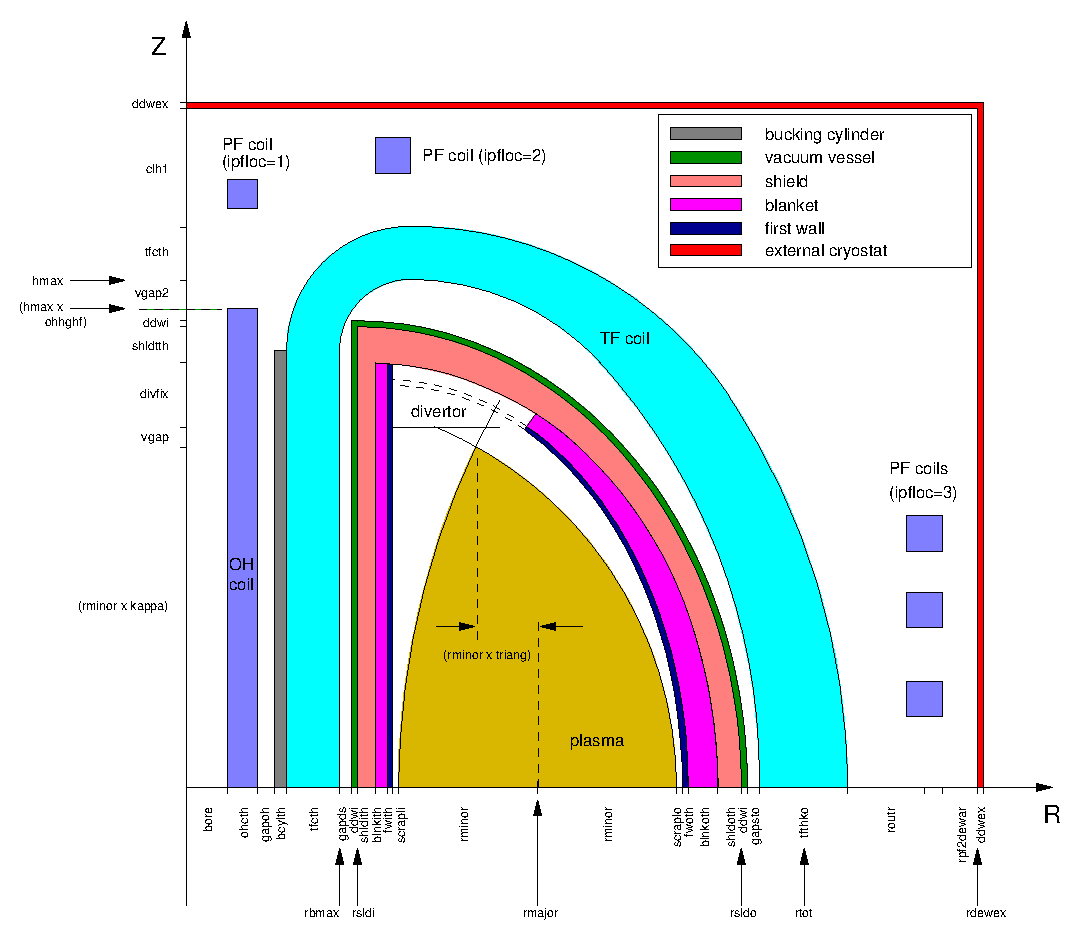
\epsfig{file=build_d.eps,width=170mm}
\caption[Machine build for D-shaped major components]
{\label{fig:build_d} \textit{Schematic diagram of the fusion
    power core of a typical tokamak power plant modelled by \process, showing
    the relative positions of the components. A double null plasma is assumed
    (\texttt{snull=0}) --- compare Figure~\ref{fig:buildsnd}, and the first
    wall, blanket, shield and vacuum vessel are D-shaped in cross-section
    (chosen by setting switch \texttt{fwbsshape=1}) --- compare
    Figure~\ref{fig:build_e}. Also shown are the code variables used to define
    the thicknesses of the components. The arrowed labels adjacent to the axes
    are the total `builds' to that point. The precise locations and sizes of
    the PF coils are calculated within the code (see
    Section~\ref{sec:pfcoils}).}  }
\end{figure}

\begin{figure}[tbph]
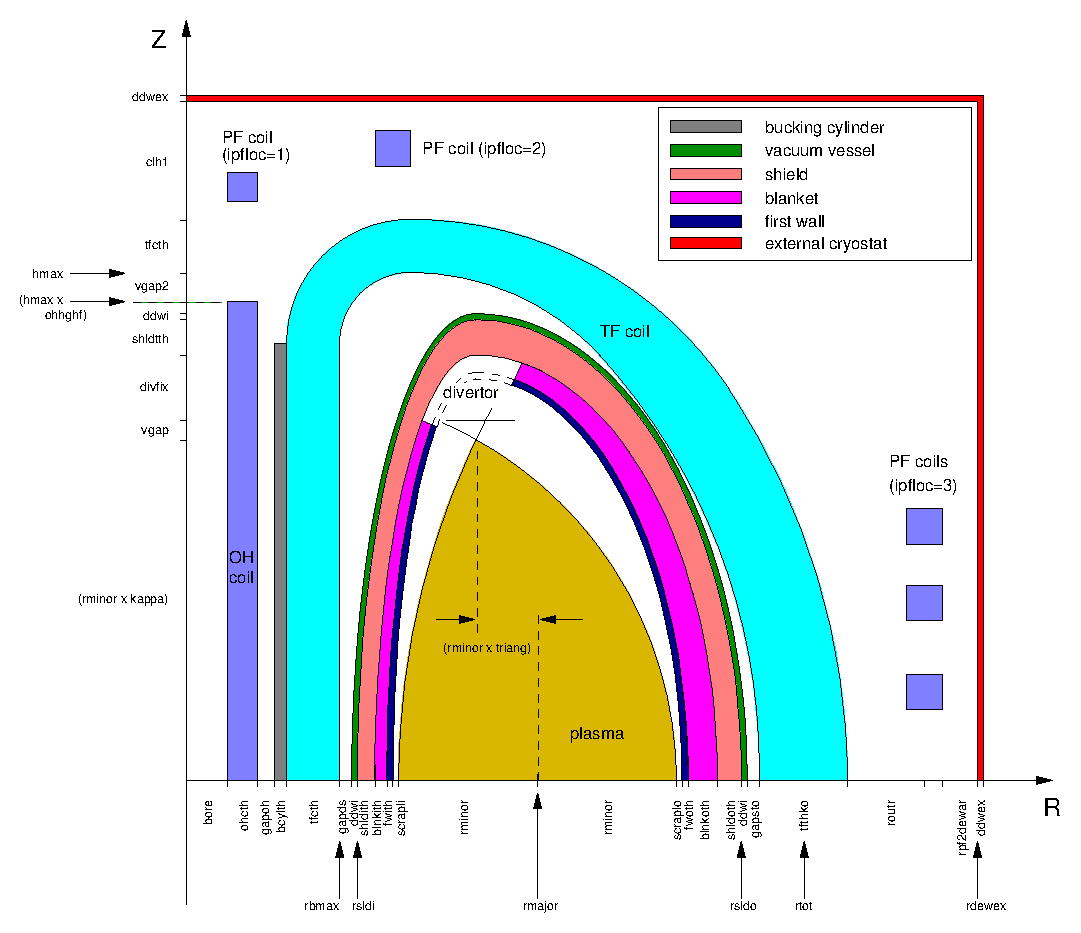
\epsfig{file=build_e.eps,width=170mm}
\caption[Machine build for elliptical-shaped major components]
{\label{fig:build_e} \textit{Schematic diagram of the fusion
    power core of a typical tokamak power plant modelled by \process. The
    first wall, blanket, shield and vacuum vessel cross-sectional shapes are
    each assumed to be defined by two ellipses (chosen by setting switch
    \texttt{fwbsshape=2}) --- compare Figure~\ref{fig:build_d}.}  }
\end{figure}

Most of the thicknesses shown in Figures~\ref{fig:build_d} and~\ref{fig:build_e}
are input parameters, so are not changed during the course of the simulation.
The rest are calculated by the code during execution. In addition, some of the
component sizes can be used as \textit{iteration variables}\/ (see
Section~\ref{sec:itvars}) to help in the optimisation process.

\begin{figure}[tbph]
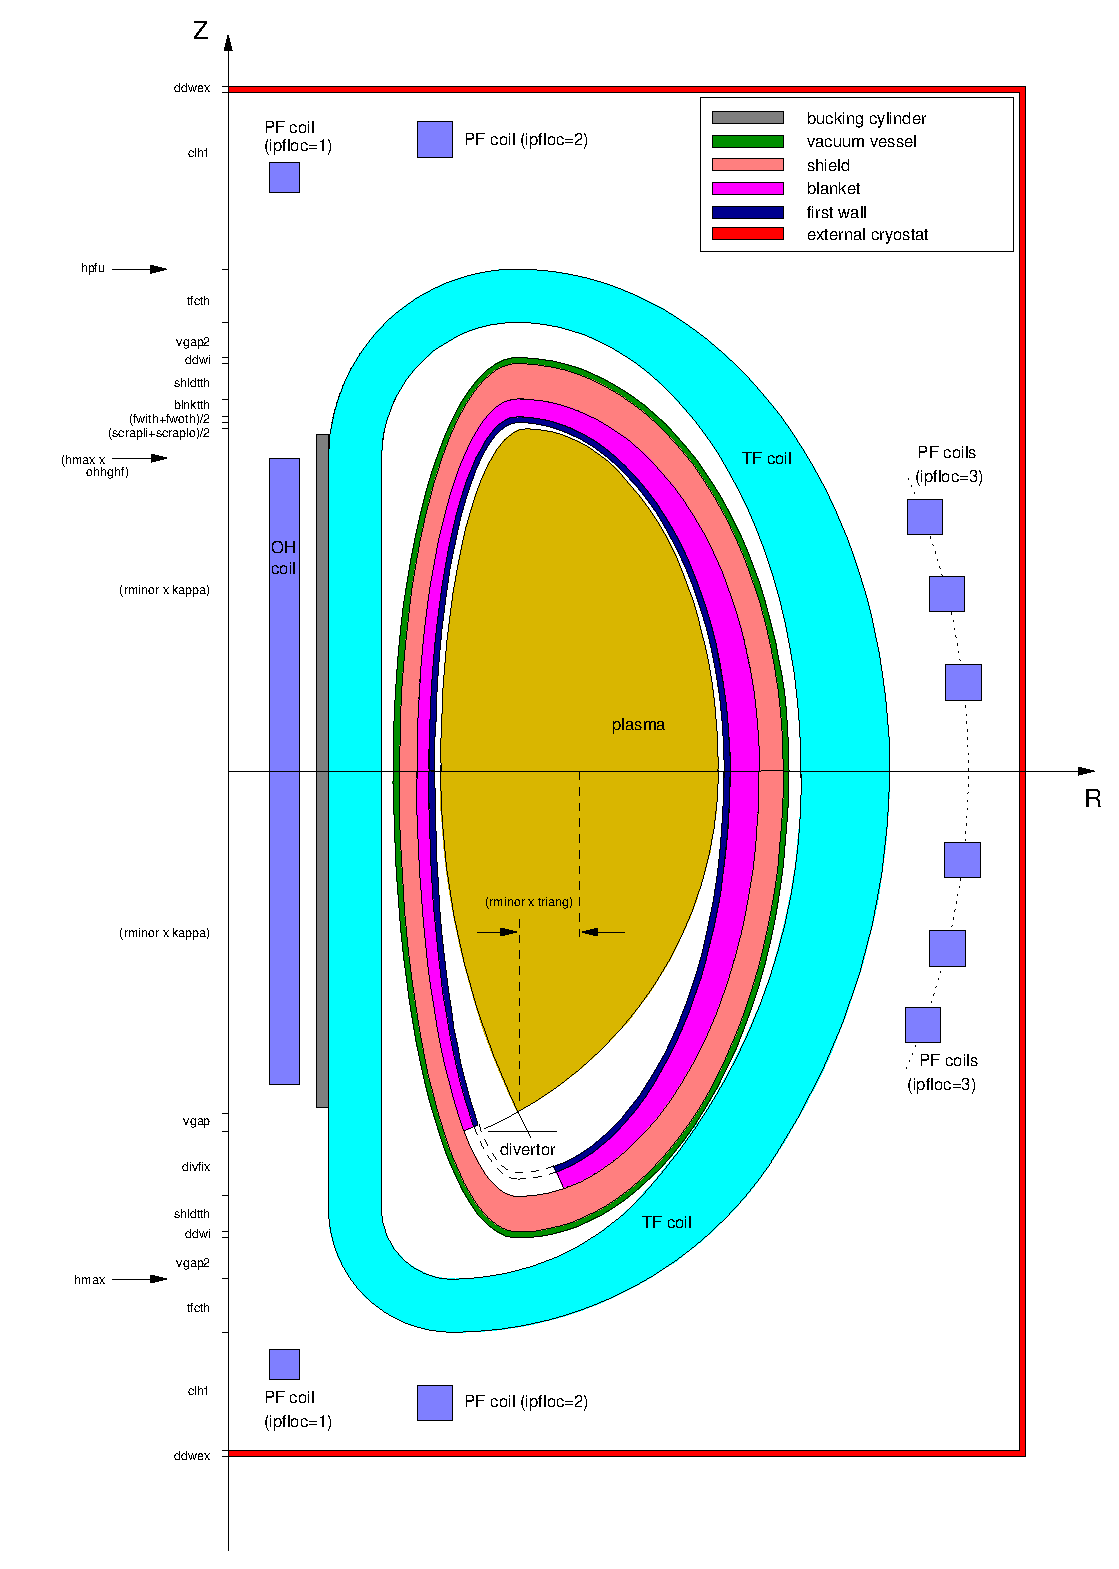
\epsfig{file=build_e_snd.eps,height=200mm}
\caption[Machine build for a single-null device]
{\label{fig:buildsnd}
  \textit{Schematic diagram of the fusion power core of a typical tokamak
    power plant modelled by \process, showing the relative positions of the
    components. A single null plasma is assumed (\texttt{snull=1}) --- compare
    Figure~\ref{fig:build_e}. The radial build is the same as for a double null
    configuration; shown along the vertical axis are the code variables used
    to define the vertical thicknesses of the components. The arrowed labels
    adjacent to the axis are the total `builds' (distance from the midplane,
    Z=0) to that point. The precise locations and sizes of the  PF coils are
    calculated within the code (see Section~\ref{sec:pfcoils}).}
}
\end{figure}

\subsection{Plasma physics models}

Arguably, the most important component of the machine is the plasma itself. By
default, this is assumed to have an up-down asymmetric, single null
configuration (although this can be changed if desired --- see
Section~\ref{sec:divertor}). A great number of physics models are coded within
\process\ to describe the behaviour of the plasma parameters such as its
current, temperature, density, pressure, confinement etc., and also the
various limits that define the stable operating domain.

\subsubsection{Plasma geometry}
\label{sec:plasma_geometry}

The plasma (geometric) major radius $R_0$ (\texttt{rmajor}) and aspect ratio
$A$ (\texttt{aspect}) define the size of the plasma torus. The plasma minor
radius $a$ (\texttt{rminor}) is calculated from these values. The shape of the
plasma cross-section is given by its last closed flux surface (LCFS) elongation
$\kappa$ (\texttt{kappa}) and triangularity $\delta$ (\texttt{triang}), which
can be scaled automatically with the aspect ratio if required using switch
\texttt{ishape}:

\begin{itemize}

\item If \texttt{ishape = 0}, the input values for \texttt{kappa} and
  \texttt{triang} are used directly.

\item If \texttt{ishape = 1}, the following scaling is used, which is suitable
  for low aspect ratio machines ($\epsilon = 1/A$)~\cite{storac}:

\begin{eqnarray}
\kappa & = & 2.05 \, (1 + 0.44 \, \epsilon^{2.1}) \\
\delta & = & 0.53 \, (1 + 0.77 \, \epsilon^3)
\end{eqnarray}

\item If \texttt{ishape = 2}, the Zohm ITER scaling~\cite{Zohm} is used to
  calculate the elongation:
\begin{equation}
\kappa = \mathrm{minimum} \left( 2.0, \, \, 1.5 + \frac{0.5}{A-1} \right)
\end{equation}
while the input value of the triangularity is used unchanged.

\end{itemize}

If \texttt{ishape = 0, 1} or \texttt{2}, the values for the plasma shaping
parameters at the 95\% flux surface are calculated as
follows~\cite{DEMOPhysicsGuidelines}:
\begin{eqnarray}
\kappa_{95} & = & \kappa / 1.12 \label{eqn:k95} \\
\delta_{95} & = & \delta / 1.5 \label{eqn:d95}
\end{eqnarray}

\begin{itemize}

\item If \texttt{ishape = 3}, the Zohm ITER scaling~\cite{Zohm} is used to
  calculate the elongation (as for \texttt{ishape = 2} above), but the
  triangularity at the 95\% flux surface is input via variable
  \texttt{triang95}, and the LCFS triangularity \texttt{triang} is calculated
  from it, rather than the other way round.

\item Finally, if \texttt{ishape = 4}, the 95\% flux surface values
  \texttt{kappa95} and \texttt{triang95} are both used as inputs, and the LCFS
  values are calculated from them by inverting Equations~\ref{eqn:k95} and~\ref{eqn:d95}.

\end{itemize}

A constraint relating to the plasma's vertical stability may be turned on if
required. In principle, the inner surface of the outboard shield could be used
as the location of a conducting shell which should mitigate the vertical
displacement growth rate of plasmas with significant
elongation~\cite{Sakamoto}. The maximum distance $r_{\mbox{\scriptsize shell,
  max}}$ of this shell from the centre of the plasma may be set using input
parameter \texttt{cwrmax}, such that $r_{\mbox{\scriptsize shell, max}} = $
\texttt{cwrmax*rminor}. Constraint equation no.\ 23 should be turned on with
iteration variable no.\ 104 (\texttt{fcwr}) to enforce this. (A scaling of
\texttt{cwrmax} with elongation should be available shortly.)

The plasma surface area, cross-sectional area and volume are calculated using
formulations that approximate the LCFS as a revolution of two arcs which
intersect the plasma X-points and the plasma midplane outer and inner
radii. (This is a reasonable assumption for double-null diverted plasmas, but
will be inaccurate for single-null plasmas, \texttt{snull = 1}.) Switch
\texttt{igeom} determines whether an old method is used (\texttt{igeom = 0})
or calculations based on a more recent derivation (\texttt{igeom =
  1})~\cite{logbook14_41}.

\subsubsection{Fusion reactions}
\label{sec:fusion_reactions}

The most likely fusion reaction to be utilised in a power plant is the
deuterium-tritium reaction:
\begin{equation}
\mathrm{D + T} \Longrightarrow \mathrm{^{4}He + n + 17.6 \,MeV}
\label{eqn:d-t}
\end{equation}
20\% of the energy produced is given to the alpha particles ($^4$He), which
remain (\Red{but c.f.\ falpha}) within the plasma and thermalise (slow down)
due to collisions, thus heating the plasma. The remaining 80\% is carried away
by the neutrons, which deposit their energy within the blanket and shield.

\process\ can also model D-$^3$He power plants, which utilise the following primary
fusion reaction:
\begin{equation}
\mathrm{D + \mbox{$^3$He}} \Longrightarrow \mathrm{^{4}He + p + 18.3 \,MeV}
\label{eqn:dhe3}
\end{equation}
The fusion reaction rate is significantly different to that for D-T fusion,
and the power flow from the plasma is modified since charged particles are
produced rather than neutrons. Because only charged particles (which remain in
the plasma) are produced by this reaction, the whole of the fusion power is
used to heat the plasma. Useful energy is extracted from the plasma since the
radiation power produced is very high, and this can be converted to
electricity in a number of ways.

Since the temperature required to ignite the D-$^3$He reaction is considerably
higher than that for D-T, it is necessary to take into account the following
D-D reactions, which have significant reaction rates at such temperatures:
\begin{eqnarray}
\mathrm{D + D} & \Longrightarrow & \mathrm{^{3}He + n + 3.27 \,MeV} \\
\mathrm{D + D} & \Longrightarrow & \mathrm{T + p + 4.03 \,MeV}
\end{eqnarray}
Also, as tritium is produced by the latter reaction, D-T fusion is also
possible. As a result, there is still a small amount of neutron power
extracted from the plasma.

Pure D-$^3$He tokamak power plants do not include blankets, because of the near
absence of neutrons leaving the plasma, and the fact that no tritium needs to
be produced for fuel.

The contributions from all four of the above fusion reactions are included in
the total fusion power production calculation. The fusion reaction rates are
calculated using the parametrizations in~\cite{BoschHale}, integrated over the
plasma profiles (correctly, with or without pedestals).

The fractional composition of the ``fuel'' ions (D, T and $^3$He) is
controlled using the three variables \texttt{fdeut}, \texttt{ftrit} and
\texttt{fhe3}, respectively:
\begin{eqnarray*}
n_{\mbox{\scriptsize fuel}} & = & n_D + n_T + n_{\mathrm{^{3}He}}  \;\;\; \mbox{particles/m$^3$} \\
n_D & = & \mathtt{fdeut} \, n_{\mbox{\scriptsize fuel}} \\
n_T & = & \mathtt{ftrit} \, n_{\mbox{\scriptsize fuel}} \\
n_{\mathrm{^{3}He}} & = & \mathtt{fhe3} \, n_{\mbox{\scriptsize fuel}}
\end{eqnarray*}
\process\ checks that \texttt{fdeut + ftrit + fhe3 = 1.0}, and stops with an
error message otherwise.

\subsubsection{Plasma profiles}

By default \Red{NOT ANY MORE!} (switch \texttt{ipedestal = 0}), the plasma
profiles are assumed to be parabolic, i.e.\ they are of the form
\begin{eqnarray}
\mbox{Density : } n(\rho) & = & n_0 \left( 1 - \rho^2 \right)^{\alpha_n} \\
\mbox{Temperature : } T(\rho) & = & T_0 \left( 1 - \rho^2 \right)^{\alpha_T} \\
\mbox{Current : } J(r) & = & J_0 \left( 1 - \rho^2 \right)^{\alpha_J}
\end{eqnarray}
where $\rho = r/a$, and $a$ is the plasma minor radius. This gives
volume-averaged values $\langle n \rangle = n_0 / (1+\alpha_n)$, and
line-averaged values $\bar{n} \sim n_0 / \sqrt{(1+\alpha_n)}$, etc.  These
volume- and line-averages are used throughout the code along with the profile
indices $\alpha$, in the various physics models, many of which are fits to
theory-based or empirical scalings. Thus, the plasma model in \process\ may
be described as ``$\frac{1}{2}$-D''.  The relevant profile index variables are
\texttt{alphan}, \texttt{alphat} and \texttt{alphaj}, respectively (see
Section~\ref{sec:current_profile}).

If \texttt{ipedestal} is set to \texttt{1}, however, the density and
temperature profiles may include a pedestal, using the forms specified
in~\cite{helios}:
\begin{equation}
\mbox{density:} \qquad n(\rho) = \left\{ 
\begin{aligned}
  &n_{ped} + (n_0 - n_{ped}) \left( 1 -
    \frac{\rho^2}{\rho_{ped,n}^2}\right)^{\alpha_n}
  &\qquad 0 \leq \rho \leq \rho_{ped,n} \\
  &n_{sep} + (n_{ped} - n_{sep})\left( \frac{1- \rho}{1-\rho_{ped,n}}\right)
  &\qquad \rho_{ped,n} < \rho \leq 1
\end{aligned}
\right.
\end{equation}

\begin{equation}
\mbox{temperature:} \qquad T(\rho) = \left\{ 
\begin{aligned}
  &T_{ped} + (T_0 - T_{ped}) \left( 1 - \frac{\rho^{\beta_T}}
    {\rho_{ped,T}^{\beta_T}}\right)^{\alpha_T} &\qquad 0 \leq \rho \leq \rho_{ped,T} \\
  &T_{sep} + (T_{ped} - T_{sep})\left( \frac{1- \rho}{1-\rho_{ped,T}}\right)
  &\qquad \rho_{ped,T} < \rho \leq 1
\end{aligned}
\right.
\end{equation}
Subscripts $0$, $ped$ and $sep$, denote values at the centre ($\rho = 0$), the
pedestal ($\rho = \rho_{ped}$) and the separatrix ($\rho=1$),
respectively. The density and temperature peaking parameters $\alpha_n$ and
$\alpha_T$ as well as the second exponent $\beta_T$ (input parameter
\texttt{tbeta}, not to be confused with the plasma beta) in the temperature
profile can be chosen by the user, as can the pedestal heights and the values
at the separatrix (\texttt{neped, nesep} for the electron density, and
\texttt{teped, tesep} for the electron temperature; the ion equivalents are
scaled from the electron values by the ratio of the volume-averaged values).
The density at the centre is given by
\begin{eqnarray}
  \nonumber
  n_0 &= & \frac{1}{3\rho_{ped,n}^2} \left[3\langle n\rangle (1+\alpha_n)
    + n_{sep} (1+\alpha_n) (-2 + \rho_{ped,n} + \rho_{ped,n}^2) \right.\\
  && \left. - n_{ped}\left( (1 + \alpha_n)(1+ \rho_{ped,n}) + (\alpha_n -2)
    \rho_{ped,n}^2 \right) \right]
\end{eqnarray}
where $\langle n \rangle$ is the volume-averaged density. The temperature at
the centre is given by
\begin{equation}
T_0 = T_{ped} + \gamma \left[ T_{ped}\, \rho_{ped,T}^2 - \langle T \rangle +
  \frac{1}{3}(1 - \rho_{ped,T}) \left[ \, (1 + 2\rho_{ped,T}) \, T_{ped} + ( 2 +
    \rho_{ped,T}) \, T_{sep} \, \right] \right]
\end{equation}
with 
\begin{equation}
\gamma = \left\{ 
\begin{aligned}
  &\frac{ -\Gamma(1+\alpha_T+2/\beta_T)}
  {\rho_{ped,T}^2 \, \Gamma(1+\alpha_T) \, \Gamma((2+\beta_T)/\beta_T)}
  &\qquad \textnormal{for integer } \alpha_T \\
  &\frac{\Gamma(-\alpha_T)\sin(\pi\alpha)\, \Gamma(1+\alpha_T+2/\beta_T)}
  {\pi\rho_{ped,T}^2 \, \Gamma((2+\beta_T)/\beta_T)}
  &\qquad \textnormal{for non-integer } \alpha_T
\end{aligned}
\right.
\end{equation}
where $\Gamma$ is the gamma function.

Note that both density and temperature can have different pedestal positions
$\rho_{ped,n}$ (\texttt{rhopedn}) and $\rho_{ped,T}$ (\texttt{rhopedt}) in
agreement with simulations.

\subsubsection{Beta limits}

The plasma beta limit~\cite{IPDG,172} is given by
\begin{equation}
\langle \beta \rangle < g \, \frac{I(\mbox{MA})}{a(\mbox{m}) \, B_0(\mbox{T})}
\label{eqn:troyon}
\end{equation}
where $B_0$ is the axial vacuum toroidal field, and $\beta$ is defined with
respect to the total equilibrium $\mathbf{B}$-field~\cite{172}. The beta
coefficient $g$ is set using input parameter \texttt{dnbeta} (but see
Section~\ref{sec:current_profile}). To apply the beta limit, constraint
equation no.\ 24 should be turned on with iteration variable no.\ 36
(\texttt{fbetatry}). The limit can be applied to either the total plasma beta,
in which case switch \texttt{iculbl} should be set to 0, to only the thermal
component of the plasma beta, in which case \texttt{iculbl} should be set to
1, or to the thermal plus neutral beam components, in which case
\texttt{iculbl} should be set to 2.

\subsubsection*{Aspect ratio scaling of beta $g$ coefficient}

Switch \texttt{gtscale} determines whether the beta $g$ coefficient
\texttt{dnbeta} should scale with aspect ratio ($\mathtt{gtscale \not= 0}$),
or be fixed at the input value (\texttt{gtscale = 0}). Note that
\texttt{gtscale} is over-ridden if \texttt{iprofile = 1} (see
Section~\ref{sec:current_profile}).

\subsubsection*{Limiting $\epsilon.\beta_p$}

To apply a limit to the value of $\epsilon.\beta_p$, where $\epsilon = a/R$ is
the inverse aspect ratio, constraint equation no.\ 6 should be turned on with
iteration variable no.\ 8 (\texttt{fbeta}). The limiting value of
$\epsilon.\beta_p$ should be set using input parameter \texttt{epbetmax}.

\subsubsection{Density limits}

Several density limit models~\cite{172} are available in \process. These are
calculated in routine \texttt{CULDLM}, which is called by \texttt{PHYSICS}.
To enforce any of these limits, turn on constraint equation no.~5 with
iteration variable no.~9 (\texttt{fdene}).  In addition, switch
\texttt{idensl} must be set to the relevant value, as follows:-
\begin{description} %!%!%! find refs
\item [\texttt{idensl = 1} :] ASDEX model
\item [\texttt{idensl = 2} :] Borrass model for ITER, I
\item [\texttt{idensl = 3} :] Borrass model for ITER, II
\item [\texttt{idensl = 4} :] JET edge radiation model
\item [\texttt{idensl = 5} :] JET simplified model
\item [\texttt{idensl = 6} :] Hugill-Murakami $M.q$ model
\item [\texttt{idensl = 7} :] Greenwald model
\end{description}

\subsubsection{Impurities and radiation}
\label{sec:radiation}

The impurity radiation model in \process\/ can be chosen using the switch
\texttt{imprad\_model}, where \texttt{imprad\_model = 0} gives the original
ITER 1989 model~\cite{kovari_physics}, and \texttt{imprad\_model = 1} uses a
multi-impurity model which integrates the radiation contributions over an
arbitrary choice of density and temperature profiles~\cite{hanni_radiation}.

If \texttt{imprad\_model = 0}, the impurity species and fractions are chosen
using input parameters \texttt{impc}, \texttt{impo}, \texttt{fbfe},
\texttt{cfe0} and \texttt{zfear}; see the variable descriptor file for more
details.

If \texttt{imprad\_model = 1}, the impurity number density fractions relative
to the electron density are set using input array \texttt{fimp(1 to nimp)},
where \texttt{nimp = 14} is the number of impurity species in the radiation
model. The available impurities are as follows:
\begin{enumerate}
\item Hydrogen (fraction calculated by code)
\item Helium (fraction calculated by code)
\item Beryllium
\item Carbon
\item Nitrogen
\item Oxygen
\item Neon
\item Silicon
\item Argon
\item Iron
\item Nickel
\item Krypton
\item Xenon
\item Tungsten
\end{enumerate}
As stated above, the number density fractions for hydrogen (all isotopes) and
helium need not be set, as they are calculated by the code to ensure that
plasma quasi-neutrality is maintained, and taking into account the fuel ratios
\texttt{fdeut}, \texttt{ftrit} and \texttt{fhe3} (see
Section~\ref{sec:fusion_reactions}), and the alpha particle fraction
\texttt{ralpne} which may be input by the user.

The impurity fraction of one of the elements listed in array \texttt{fimp} may
be used as an iteration variable (although it will only have any effect if
\texttt{imprad\_model = 1}). The element to use is specified using input
parameter \texttt{impvar}, which may be set to a value between 3 and
\texttt{nimp}, and the initial estimate to use for the element's impurity
fraction must be set using iteration variable no.\ 102 (\texttt{fimpvar}).

The synchrotron radiation power~\cite{albajar, fidone} is assumed to originate
from the plasma core. The wall reflection factor \texttt{ssync} may be set by
the user.

By changing the input parameter \texttt{coreradius}, the user may set the
normalised radius defining the core region (\texttt{imprad\_model = 1}
only). Only the impurity and synchrotron radiation from the core region
affects the confinement scaling (but see \texttt{iradloss} below), while the
power flowing into the divertor is assumed to exclude all radiation power.

\Red{Add radiation power flow diagram as on p.26, logbook24}

\Red{New overall power flow diagram should elucidate this...}

Constraint equation no.~17 with iteration variable no.~28 (\texttt{fradpwr})
ensures that the calculated total radiation power does not exceed the total
power available that can be converted to radiation (i.e.\ the sum of the fusion
alpha power, other charged particle fusion power, auxiliary injected power and
the ohmic power). This constraint should always be turned on.

Switch \texttt{iradloss} may be used to exclude (\texttt{iradloss = 1},
default) or include (\texttt{iradloss = 0}) the core radiation power in the
transport power used in the confinement time and power balance calculations
(see Section~\ref{sec:corepower}).

\subsubsection{Plasma current scaling laws}
\label{sec:current_scaling}

A number of plasma current scaling laws exploiting the inverse relationship
between plasma current and edge safety factor $q_{\psi}$~\cite{172} are
available in \process. These are calculated in routine \texttt{CULCUR}, which
is called by \texttt{PHYSICS}.  Flag \texttt{icurr} must be set to the
relevant value, as follows:-
\begin{description}
\item [\texttt{icurr = 1} :] Peng analytic fit
\item [\texttt{icurr = 2} :] Peng double null divertor scaling (ST)~\cite{storac}
\item [\texttt{icurr = 3} :] Simple ITER scaling
\item [\texttt{icurr = 4} :] Revised ITER scaling~\cite{Uckan88}
\item [\texttt{icurr = 5} :] Todd empirical scaling, I
\item [\texttt{icurr = 6} :] Todd empirical scaling, II
\item [\texttt{icurr = 7} :] Connor-Hastie model
\end{description}

\subsubsection{Plasma current profile consistency}
\label{sec:current_profile}

Self-consistency between the plasma current profile
parameters~\cite{DEMOPhysicsGuidelines} can be enforced by setting switch
\texttt{iprofile} to 1. This ensures that the current profile peaking factor
\texttt{alphaj} is consistent with the input values for the safety factor on
axis and at the plasma edge (\texttt{q0} and \texttt{q}, respectively), the
plasma internal inductance $l_i$ is consistent with this \texttt{alphaj}, and
the beta $g$ coefficient \texttt{dnbeta} scales with $l_i$.

It is recommended that current scaling law \texttt{icurr = 4} is used if
\texttt{iprofile = 1}. Switch \texttt{gtscale} is over-ridden if
\texttt{iprofile = 1}.

\subsubsection{Confinement time scaling laws}
\label{sec:taue}

The particle transport loss power in Watts/m$^3$ from the plasma is defined as
\begin{equation}
P_{\mbox{\scriptsize loss}} = \frac{W}{\tau_E}
\label{eqn:ploss}
\end{equation}
where the plasma stored energy per unit volume $W$ is given by
\[
W = \frac{3}{2} \,n \, e \, T
\]
with particle number density $n$ in m$^{-3}$ and particle temperature $T$ in
eV. \process\ assumes that the electron and ion energy confinement times
$\tau_E$ are equal.

Many energy confinement time scaling laws are present within \process, for
tokamaks, RFPs or stellarators. These are calculated in routine
\texttt{PCOND}. The value of \texttt{isc} determines which of the scalings is
used in the plasma energy balance calculation (Section~\ref{sec:corepower}).
Table~\ref{tab:scaling_laws} summarises the available scaling laws.

% Table summarising confinement time scaling laws in PROCESS.
\begin{table}[tbph]
\begin{center}
\footnotesize
\begin{tabular}{||c||l|l||} \hline
\texttt{isc} & scaling law & reference \\ \hline
\texttt{1}  & Neo-Alcator (ohmic) & \cite{IPDG} \\
\texttt{2}  & Mirnov (H-mode) & \cite{IPDG} \\
\texttt{3}  & Merezhkin-Muhkovatov (L-mode) & \cite{IPDG} \\
\texttt{4}  & Shimomura (H-mode) & JAERI-M 87-080 (1987) \\
\texttt{5}  & Kaye-Goldston (L-mode) & Nuclear Fusion \textbf{25} (1985) p.65 \\
\texttt{6}  & ITER 89-P (L-mode) & Nuclear Fusion \textbf{30} (1990) p.1999 \\
\texttt{7}  & ITER 89-O (L-mode) & \cite{IPDG} \\
\texttt{8}  & Rebut-Lallia (L-mode) & Plasma Physics and Controlled Nuclear Fusion
Research \\
 & &  \textbf{2} (1987) p. 187 \\
\texttt{9}  & Goldston (L-mode) & Plas.\ Phys.\ Controlled Fusion \textbf{26} (1984) p.87 \\
\texttt{10} & T10 (L-mode) & \cite{IPDG} \\
\texttt{11} & JAERI-88 (L-mode) & JAERI-M 88-068 (1988) \\
\texttt{12} & Kaye-Big Complex (L-mode) & Phys.\ Fluids B \textbf{2} (1990) p.2926 \\
\texttt{13} & ITER H90-P (H-mode) &  \\
\texttt{14} & ITER Mix (minimum of \texttt{6} and \texttt{7}) &  \\
\texttt{15} & Riedel (L-mode) &  \\
\texttt{16} & Christiansen et al. (L-mode) & JET Report JET-P (1991) 03 \\
\texttt{17} & Lackner-Gottardi (L-mode) & Nuclear Fusion \textbf{30} (1990) p.767  \\
\texttt{18} & Neo-Kaye (L-mode) & \cite{IPDG} \\
\texttt{19} & Riedel (H-mode) &  \\
\texttt{20} & ITER H90-P (amended) & Nuclear Fusion \textbf{32} (1992) p.318 \\
\texttt{21} & Large Helical Device (stellarator) & Nuclear Fusion \textbf{30} (1990)
p.11 \\
\texttt{22} & Gyro-reduced Bohm (stellarator) & Bull. Am. Phys. Society, \textbf{34}
(1989) p.1964 \\
\texttt{23} & Lackner-Gottardi (stellarator) & Nuclear Fusion \textbf{30} (1990) p.767 \\
\texttt{24} & ITER-93H (H-mode) & Plasma Physics and Controlled Nuclear Fusion
Research \\
 & & (Proc. 15th Int. Conf., Seville, 1994) IAEA-CN-60/E-P-3 \\
\texttt{25} & TITAN (RFP) & TITAN RFP Fusion Reactor Study, Scoping Phase
Report \\
 & & UCLA-PPG-1100, page 5--9, Jan 1987 \\
\texttt{26} & ITER H-97P ELM-free (H-mode) & J. G. Cordey et al., EPS
Berchtesgaden, 1997 \\
\texttt{27} & ITER H-97P ELMy (H-mode) & J. G. Cordey et al., EPS
Berchtesgaden, 1997 \\
\texttt{28} & ITER-96P (= ITER97-L) (L-mode) & Nuclear Fusion \textbf{37} (1997) p.1303 \\
\texttt{29} & Valovic modified ELMy (H-mode) &  \\
\texttt{30} & Kaye PPPL April 98 (L-mode) &  \\
\texttt{31} & ITERH-PB98P(y) (H-mode) &  \\
\texttt{32} & IPB98(y) (H-mode) & Nuclear Fusion \textbf{39} (1999) p.2175 \\
\texttt{33} & IPB98(y,1) (H-mode) & Nuclear Fusion \textbf{39} (1999) p.2175 \\
\texttt{34} & IPB98(y,2) (H-mode) & Nuclear Fusion \textbf{39} (1999) p.2175 \\
\texttt{35} & IPB98(y,3) (H-mode) & Nuclear Fusion \textbf{39} (1999) p.2175 \\
\texttt{36} & IPB98(y,4) (H-mode) & Nuclear Fusion \textbf{39} (1999) p.2175 \\
\texttt{37} & ISS95 (stellarator) & Nuclear Fusion \textbf{36} (1996) p.1063 \\
\texttt{38} & ISS04 (stellarator) & Nuclear Fusion \textbf{45} (2005) p.1684 \\
\texttt{39} & DS03 (H-mode) & Plasma Phys.\ Control.\ Fusion \textbf{50} (2008) 043001, equation 4.13 \\
\hline
\end{tabular}
\normalsize
\end{center}
\caption[List of available energy confinement scaling laws]
{\label{tab:scaling_laws}
  \textit{Summary of the energy confinement time scaling laws in \process.}
}
\end{table}

\subsubsection{Plasma core power balance}
\label{sec:corepower}

Figure~\ref{fig:powerflow1} shows schematically the flow of power within the
plasma as calculated by the code. (Figures~\ref{fig:powerflow2} and
\ref{fig:powerflow3} show the power transfer mechanisms for the remainder of
the power plant.)

\begin{figure}[tbph]
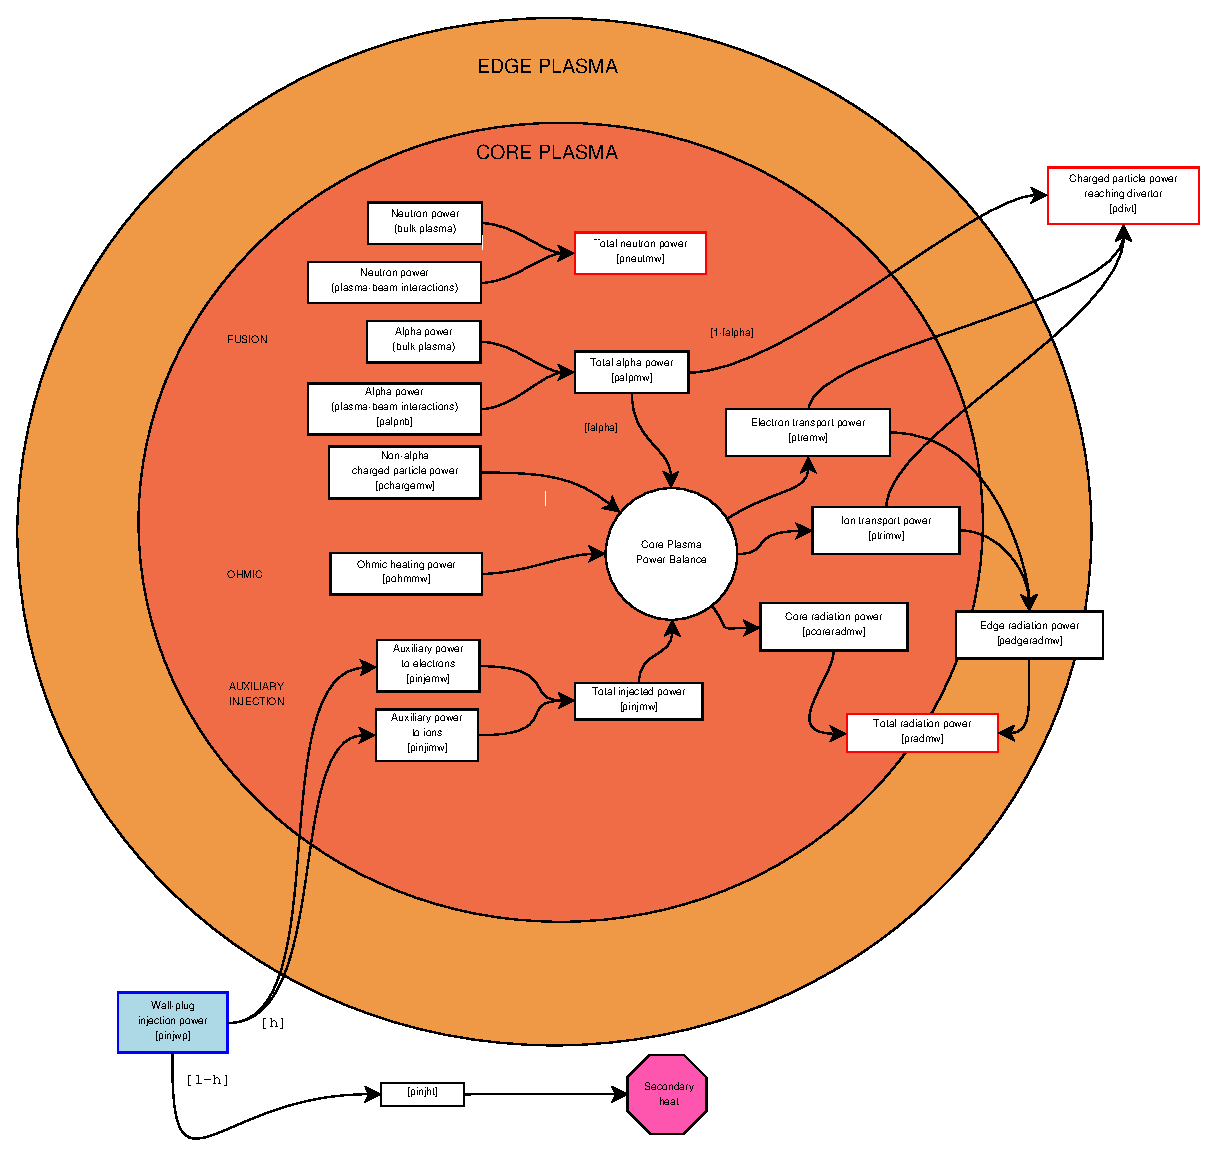
\epsfig{file=powerflow1.eps,width=170mm}
\caption[Power balance within the core plasma] {\label{fig:powerflow1}
  \textit{Schematic diagram of the flow of power within the plasma
    core. Variable names are given in [\ldots]. Refer to
  Figure~\ref{fig:powerflow2} for the onward flow of power from the three
  red-bordered boxes, while the source of the power in the blue box is
  indicated in Figure~\ref{fig:powerflow3}.} }
\end{figure}

The primary sources of power are the fusion reactions themselves, ohmic power
due to resistive heating within the plasma, and any auxiliary power provided
for heating and current drive (see Section~\ref{sec:hcd}). The power carried
by the fusion-generated neutrons is lost from the plasma, but is deposited in
the surrounding material (see Section~\ref{sec:powerflow}). A fraction
\texttt{falpha} of the alpha particle power is assumed to stay within the
plasma core to contribute to the plasma power balance. The sum of this core
alpha power, any power carried by non-alpha charged particles, the ohmic power
and any injected power, is converted into charged particle transport power
($P_{\mbox{\scriptsize loss}}$ in Equation~\ref{eqn:ploss}) plus core
radiation power (see Section~\ref{sec:radiation}), as shown in
Figure~\ref{fig:powerflow1}. (Note that, if switch \texttt{iradloss} is set to
zero, the above summed input power is converted into charged particle
transport power only, and the core radiation power may be assumed to originate
from the transport power; i.e.\ the core radiation power is treated the same
as the edge radiation power in Figure~\ref{fig:powerflow1} instead of having
an arrow leading directly to it from the core plasma power balance.)

The core power balance calculation is turned on using constraint equation
no.\ 2 (which should therefore always be used).

\subsubsection{Bootstrap current scalings}
\label{sec:bootstrap}

The fraction of the plasma current provided by the so-called bootstrap effect
can be either input into the code directly, or calculated using one of four
methods, as summarised here. Note that methods \texttt{ibss = 1} to~\texttt{3}
use fits to parabolic density and temperature profiles, and do not take into
account the existence of pedestals (\texttt{ipedestal = 1}), whereas the
Sauter et al.\ scaling (\texttt{ibss = 4}) allows general profiles to be used.

\begin{itemize}

\item Direct input: To input the bootstrap current fraction directly, set
  \texttt{bscfmax} to $(-1)$ times the required value.

\item ITER scaling~\cite{IPDG}: To use the ITER scaling method for the
  bootstrap current fraction, set \texttt{ibss = 1}, and \texttt{bscfmax} to
  the maximum required bootstrap current fraction ($\leq 1$). This method is
  valid at high aspect ratio only.

\item General scaling~\cite{Nevins}: To use a more general scaling method, set
  \texttt{ibss = 2}, and \texttt{bscfmax} to the maximum required bootstrap
  current fraction ($\leq 1$).

\item Numerically fitted scaling~\cite{WilsonBS}: To use a numerically fitted
  scaling method, valid for all aspect ratios, set \texttt{ibss = 3}, and
  \texttt{bscfmax} to the maximum required bootstrap current fraction ($\leq
  1$).

\item Sauter, Angioni and Lin-Liu scaling~\cite{SauterBS, SauterBS_errata}:
  Set \texttt{ibss = 4}, and \texttt{bscfmax} to the maximum required
  bootstrap current fraction ($\leq 1$).

\end{itemize}

\subsubsection{L-H power threshold scalings}

Transitions from a standard confinement mode (L-mode) to an improved
confinement regime (H-mode), called L-H transitions, are observed in most
tokamaks. A range of scaling laws are available that provide estimates of the
auxiliary power required to initiate these transitions, via extrapolations
from present-day devices. \process\ calculates these power threshold values
for the scaling laws listed in Table~\ref{tab:power_thresholds}, in
routine~\texttt{PTHRESH}.

To enforce one of these scalings, use input parameter \texttt{ilhthresh} to
select the scaling to use, and turn on constraint equation no.\ 23 with
iteration variable no.\ 104 (\texttt{flhthresh}). By default, this will ensure
that the power reaching the divertor is at least equal to the threshold power
calculated for the chosen scaling, which is a necessary condition for
H-mode. However, for L-mode it might be appropriate to set \texttt{boundl(104)
  = 0.001, boundu(104) = 1.0}, which will ensure that the power threshold does
not exceed the calculated value, and therefore the machine cannot reach
H-mode.

% Table summarising L-H power threshold scalings

\begin{table}[tbph]
\small
\begin{center}
\begin{tabular}{||c||l||l||} \hline
 & name & reference \\ \hline
(1) & 1996 ITER scaling: nominal & ITER Physics Design Description Document, \\
(2) & 1996 ITER scaling: upper bound & D. Boucher, p.2-2 \\
(3) & 1996 ITER scaling: lower bound &  \\ \hline
(4) & 1997 ITER scaling, excluding elongation & J. A. Snipes, ITER H-mode
Threshold Database \\
(5) & 1997 ITER scaling, including elongation &  Working Group, Controlled
Fusion and Plasma \\
 & & Physics, 24th EPS Conference, Berchtesgaden, \\
 & & June 1997, vol.21A, part III, p.961 \\ \hline
(6) & 2008 Martin scaling: nominal & Martin et al, 11th IAEA Tech. Meeting on
H-mode \\
(7) & 2008 Martin scaling: 95\% upper bound &  Physics and Transport Barriers,
Journal of Physics: \\
(8) & 2008 Martin scaling: 95\% lower bound & Conference Series \textbf{123}
(2008) 012033 \\
\hline
\end{tabular}
\end{center}
\normalsize
\caption[List of available L-H power threshold scalings]
{\label{tab:power_thresholds}
  \textit{Summary of the L-H power threshold scalings implemented in \process.}
}
\end{table}

\subsubsection{Other plasma physics options}

\subsubsection*{Neo-classical correction effects}

Switch \texttt{ires} controls whether neo-classical correction
effects~\cite{Uckan} are included in the calculation of the plasma resistance
and ohmic heating power in routine \texttt{POHM}, which is called by routine
\texttt{PHYSICS}. If \texttt{ires = 1}, these effects are included. Note that
the scaling used is only valid for aspect ratios between 2.5 and 4, and it is
possible for the plasma resistance to be wrongly calculated as negative if
\texttt{ires = 1} and the aspect ratio is too high.

\subsubsection*{Inverse quadrature in $\tau_E$ scaling laws}

Switch \texttt{iinvqd} determines whether the energy confinement time scaling
laws (see Section~\ref{sec:taue}) due to Kaye-Goldston (\texttt{isc = 5}) and
Goldston (\texttt{isc = 9}) should include an inverse quadrature scaling with
the Neo-Alcator result (\texttt{isc = 1}). A value \texttt{iinvqd = 1}
includes this scaling.

\subsubsection*{Plasma / first wall gap}

The region directly outside the last closed flux surface of the core plasma is
known as the scrape-off layer, and contains no structural material.  Plasma
entering this region is not confined and is removed by the divertor. \process\
treats the scrape-off layer merely as a gap. Switch \texttt{iscrp} determines
whether the inboard and outboard gaps should be calculated as 10\% of the
plasma minor radius (\texttt{iscrp = 0}), or set equal to the input values
\texttt{scrapli} and \texttt{scraplo} (\texttt{iscrp = 1}).

\subsection{First wall}

The first wall acts as a physical barrier protecting the rest of the machine
from the hot plasma. Due to its hostile environment the first wall has only a
short lifetime and therefore needs to be replaced regularly. Its stainless
steel structure is cooled either by gaseous helium or by pressurised water, as
chosen using switch \texttt{costr} -- see Section~\ref{sec:blanket}.

The first wall coolant fraction is given by the value of \texttt{fwclfr},
which is calculated if a pulsed power plant is being modelled (\texttt{lpulse
  = 1} --- see Section~\ref{sec:pulsed}), and assumed to be the input value
otherwise.

\subsubsection*{Wall load calculation}

Switch \texttt{iwalld} determines whether the neutron wall load (power per
unit area) should be calculated using the plasma surface area (\texttt{iwalld
  = 1}) or the first wall area (\texttt{iwalld = 2}) as the denominator. In
the former case, input parameter \texttt{ffwal} (default value 0.92)
can be used to scale the neutron power reaching the first wall.

\subsection{Divertor}
\label{sec:divertor}

The divertor provides a means of removing plasma reaching the scrape-off layer
and heavy ions that are ejected from the first wall.  By default, two
divertors are assumed in the \process\ tokamak, placed symmetrically above
and below the plasma. The principal outputs from the code are the divertor
heat load, used to determine its lifetime, and its peak temperature. The
divertor is cooled either by gaseous helium or by pressurised water.

Switch \texttt{snull} controls the overall plasma configuration. Setting
\texttt{snull = 0} corresponds to an up-down symmetric, double null
configuration (the default), while \texttt{snull = 1} assumes a single null
plasma with the divertor at the bottom of the machine. The vertical build (see
Figure~\ref{fig:buildsnd}) and PF coil current scaling algorithms take the
value of this switch into account, although not the plasma geometry at
present.

The Harrison-Kukushkin-Hotston divertor model~\cite{IPDG} developed for ITER
is used (except for the case of spherical tokamaks or stellarators --- see
later). This is appropriate for conventional aspect ratio machines, but care
should be taken in inputting the divertor magnetics for this model, and
projections far from the ITER CDA machine parameters are likely to be
unreliable.

\subsection{Blanket}

The blanket performs a number of tasks. An incoming neutron from a
deuterium-tritium (D-T) fusion reaction in the plasma loses energy in the
blanket. This energy is removed by the blanket coolant and used to produce
electricity. The neutron may also react with a lithium nucleus present in the
blanket to produce (``breed'') a tritium nucleus which can be re-used as
fuel. The competing requirements of heating and tritium synthesis mean that a
neutron multiplier must be present, to ensure balance between tritium
destruction and creation. The blanket therefore contains beryllium to fulfil
this purpose. As with the first wall, the blanket has a relatively short
lifetime because of the high neutron fluence.

\subsubsection{Blanket neutronics model}
\label{sec:blanket_neutronics}

Switch \texttt{blktmodel} determines whether a simple blanket neutronics model
or a more comprehensive treatment based on recent full neutronics analyses for
EFDA~\cite{efda_blanket_model} is used.

In the simple model (\texttt{blktmodel = 0}), the overall radial thicknesses
of the inboard and outboard blanket sections are specified via input
parameters \texttt{blnkith} and \texttt{blnkoth}, respectively. The energy
multiplication in the blanket (\texttt{emult}) is also an input
parameter. Steel and vanadium may be used as structural materials within the
blanket, which is cooled either by gaseous helium or by pressurised water. The
nuclear heating of the TF coil superconductor is calculated assuming an
exponential neutron attenuation through the blanket and shield materials,
based on 1990 ITER data.

The more advanced model (\texttt{blktmodel = 1}) allows the energy
multiplication factor \texttt{emult}, the shielding requirements and tritium
breeding ratio to be calculated self-consistently with the blanket and
shielding materials and sub-assembly thicknesses, and for constraints to be
applied to satisfy the engineering requirements. The rest of this section
describes this model in more detail.

The model is based on the Helium-Cooled Pebble Bed (HCPB) blanket concept
developed by KIT (a second advanced model --- Helium-Cooled Lithium Lead, HCLL
--- will be implemented in due course). The blanket, shield and vacuum vessel
are segmented radially into a number of sub-assemblies. Moving in the
direction away from the plasma/first wall, these are:

\begin{itemize}

\item Breeding Zone (BZ) (which includes the first wall), with radial
  thicknesses (inboard and outboard, respectively) \texttt{fwith+blbuith},
  \texttt{fwoth+blbuoth}. This consists of beryllium (with fraction by volume
  \texttt{fblbe}), breeder material (\texttt{fblbreed}), steel
  (\texttt{fblss}) and helium coolant. Three forms of breeder material are
  available: lithium orthosilicate (Li$_4$SiO$_4$) (chosen by setting
  \texttt{breedmat = 1}), lithium metatitanate (Li$_2$TiO$_3$)
  (\texttt{breedmat = 2}) or lithium zirconate (Li$_2$ZrO$_3$)
  (\texttt{breedmat = 3}). The $^6$Li enrichment percentage may be modified
  from the default 30\% using input parameter \texttt{li6enrich}.

\item Box Manifold (BM), with radial thicknesses (inboard and outboard,
  respectively) \texttt{blbmith}, \texttt{blbmoth} and helium fractions
  \texttt{fblhebmi}, \texttt{fblhebmo} (the rest being steel).

\item Back Plate (BP), with radial thicknesses (inboard and outboard,
  respectively) \texttt{blbpith}, \texttt{blbpoth} and helium fractions
  \texttt{fblhebpi}, \texttt{fblhebpo} (the rest being steel).

Together, the BZ, BM and BP make up the `blanket', with total radial
thicknesses \texttt{blnkith} (inboard) and \texttt{blnkoth} (outboard), and
void (coolant) fraction \texttt{vfblkt}; Note that these
quantities are \textit{calculated}\ from the sub-assembly values if
\texttt{blktmodel > 0}, rather than being input parameters.

\item Low Temperature Shield and Vacuum Vessel (lumped together for these
  calculations), with radial thicknesses (inboard and outboard, respectively)
  \texttt{shldith+ddwi}, \texttt{shldoth+ddwi} and \textbf{water} coolant
  fraction \texttt{vfshld} (the rest being assumed to be steel for its mass
  calculation; the neutronics model assumes that the shield contains 2\% boron
  as a neutron absorber, but this material is not explicitly mentioned
  elsewhere in the code --- so its cost is not calculated, for example).

  \textit{N.B.\ The fact that water is assumed to be the coolant in the
    shield, whereas helium is the coolant in the blanket, leads to an
    inconsistency when specifying the coolant type via switch \texttt{costr}
    (see Section~\ref{sec:blanket}). At present we mitigate this by forcing
    \texttt{costr=2} (making water the coolant), as in this case the coolant
    mass and pumping costs are higher, giving the more pessimistic solution
    with regards to costs.}

\end{itemize}

A few other input parameters are useful for tuning purposes, as follows:

\begin{itemize}

\item \texttt{fhole} is the `hole' area fraction of the first wall and blanket
  that neutrons leaving the plasma see, due to the presence of the divertor,
  for instance. That is, \texttt{1-fhole} is the first wall area coverage
  factor. \Red{(N.B.\ see Section~\ref{sec:powerflow}.)}

\item \texttt{fvolsi} and \texttt{fvolso} are the area (and volume) coverage
  factors for the inboard and outboard shields, respectively.

\item \texttt{fvoldw} is a multiplier for the volume of the vacuum vessel,
  used in the item's mass calculation to account for ports, etc.

\item \texttt{npdiv} is the number of divertor ports, used in the calculation
  of the tritium breeding ratio (\texttt{blktmodel > 0} only).

\item \texttt{nphcdin} and \texttt{nphcdout} are the number of heating/current
  drive ports on the inboard and outboard sides, respectively, used in the
  calculation of the tritium breeding ratio (\texttt{blktmodel > 0}
  only). These may be either `small' (\texttt{hcdportsize = 1}) or `large'
  (\texttt{hcdportsize = 2}).

\item \texttt{wallpf} is the neutron wall load peaking factor (maximum/mean),
  used in the calculation of the blanket lifetime (\texttt{blktmodel > 0}
  only).

\item \texttt{ucblbreed} is the unit cost (\$/kg) of the breeder material
  (\texttt{blktmodel > 0} only).

\end{itemize}

\subsubsection*{Model outputs and available constraints}

The advanced blanket neutronics model provides the following outputs:

\begin{itemize}

\item The total nuclear power deposited in the blanket and shield,
  \texttt{pnucblkt} and \texttt{pnucshld}, respectively, and the energy
  multiplication factor in the blanket, \texttt{emult} are calculated.

\item The tritium breeding ratio, \texttt{tbr}. This can be constrained to be
  no less than a certain value \texttt{tbrmin} for tritium self-sufficiency by
  turning on constraint equation no.\ 52 with iteration variable no.\ 89
  (\texttt{ftbr}). The inboard and outboard blanket BZ thicknesses,
  \texttt{blbuith} and \texttt{blbuoth} can also be used as iteration
  variables (90 and 91, respectively) to help the constraint to be met.

\item The tritium production rate in grammes/day is calculated.

\item The fast neutron fluence (neutrons/m$^2$) on the TF coils is
  calculated. The peak value of this quantity may be constrained to be no more
  than a maximum value \texttt{nflutfmax} by turning on constraint equation
  no.\ 53 with iteration variable no.\ 92 (\texttt{fflutf}). The inboard and
  outboard shield thicknesses, \texttt{shldith} and \texttt{shldoth} can also
  be used as iteration variables (93 and 94, respectively) to help the
  constraint to be met. (Note that in this calculation the TF coil case
  surrounding the superconductor winding pack is ignored.)

\item The nuclear heating power (MW/m$^3$) on the inboard and outboard TF
  coils is calculated. Again, this can be limited to be no more than a maximum
  value \texttt{ptfnucmax} by turning on constraint equation no.\ 54 with
  iteration variable no.\ 95 (\texttt{fptfnuc}). The inboard and outboard
  shield thicknesses also help this constraint to be met.  (Note that in this
  calculation the TF coil case surrounding the superconductor winding pack is
  ignored.) This constraint equation may also be used with \texttt{blktmodel =
    0}.

\item The helium concentration in the vacuum vessel at the end of the plant
  lifetime is calculated. This needs to be constrained for re-weldability
  purposes, and can be kept below a maximum value \texttt{vvhealw} by turning
  on constraint equation no.\ 55 with iteration variable no.\ 96
  (\texttt{fvvhe}).

\item The blanket lifetime is calculated, assuming a maximum allowable level
  of neutron damage to its steel of 60~dpa (currently not adjustable). (For
  the \texttt{blktmodel = 0} model, the allowable blanket fluence
  \texttt{abktflnc} in MW-years/m$^2$ may be input.)

\end{itemize}

\subsubsection{Full thermodynamic blanket model}
\label{sec:blanket}

\Red{Remove asap.}

\textbf{N.B.\ it is recommended that this model is \textit{not}\ used in
  conjunction with the advanced blanket neutronics model (\texttt{blktmodel >
    0}).}

Switch \texttt{lblnkt} determines whether the blanket is to be simulated using
a full thermodynamic model~\cite{Panos} (\texttt{lblnkt = 1}), or simply
assumed to be made up of relevant materials (see
Section~\ref{sec:blanket_materials}) in user-defined proportions. The former
model also performs a self-consistent calculation of the thermal-to-electric
conversion efficiency, whereas the latter simply uses the input value
\texttt{etath}.

The following switches control the details of the full thermodynamic model of
the blanket.

\begin{itemize}

\item \textbf{Cooling channel geometry:} The value of switch \texttt{astr}
  determines whether the cooling channels have a circular cross-section
  (\texttt{astr = 1}) or an annular cross-section (\texttt{astr = 2}). The
  latter case is the default.

\item \textbf{Cooling channel orientation:} The value of switch \texttt{estr}
  determines whether the cooling channels lie in the radial direction
  (\texttt{estr = 1}) or in the poloidal direction (\texttt{estr = 2}). The
  former case is the default.

\item \textbf{Coolant type:} The value of switch \texttt{costr} determines the
  type of coolant used in the first wall, blanket and shield. If \texttt{costr
    = 1}, the coolant is assumed to be gaseous helium. If \texttt{costr = 2},
  the coolant is assumed to be pressurised water/steam, which is the
  default. This switch is used whether or not the full blanket model is used,
  i.e.\ is independent of the setting of switch \texttt{lblnkt}.

\item \textbf{Boundary condition:} The value of switch \texttt{bstr}
  determines whether the coolant output temperature is to be fixed
  (\texttt{bstr = 1}) or whether the maximum blanket temperature is to be
  fixed (\texttt{bstr = 2}). The former case is the default.  The desired
  coolant output temperature for \texttt{bstr = 1} is set using input
  parameter \texttt{xtfo}, and the required maximum blanket temperature is set
  using input parameter \texttt{xtb}.

\end{itemize}

\subsubsection{Blanket materials}
\label{sec:blanket_materials}

Table~\ref{tab:blanket} summarises the possible options for the blanket
materials. Switch \texttt{smstr} determines whether a solid blanket of
Li$_2$O-Be (\texttt{smstr = 1}), or a liquid blanket of LiPb-Li (\texttt{smstr
  = 2}) is used. The former is the default, and is the type assumed if
$\mathtt{lblnkt \not= 1}$.

% Table summarising blanket materials

\begin{table}[tbph]
\begin{center}

\begin{tabular}{||l||c||c||c||} \hline
material & $\mathtt{lblnkt \not= 1}$: & \multicolumn{2}{c||}{\texttt{lblnkt = 1}: full
thermodynamic model} \\ \cline{3-4}
 & simple model & \texttt{smstr=1}: solid blanket & \texttt{smstr=2}: liquid blanket
\\ \hline
stainless steel & \texttt{fblss}   & \texttt{fblss}   & \texttt{fblss}   \\
vanadium        & \texttt{fblvd}   & \texttt{fblvd}   & \texttt{fblvd}   \\
Li$_2$O         & \texttt{fblli2o} & \texttt{fblli2o} &     ---       \\
beryllium       & \texttt{fblbe}   & \texttt{fblbe}   &     ---       \\
LiPb            &     ---       &     ---       & \texttt{fbllipb} \\
lithium         &     ---       &     ---       & \texttt{fblli}   \\
coolant         & \texttt{vfblkt}  & \texttt{vfblkt}  & \texttt{vfblkt}  \\ \hline
\end{tabular}
\end{center}
\caption[Summary of blanket material scenarios]
{\label{tab:blanket}
  \textit{Summary of the materials comprising the blanket in the various scenarios
    available (\texttt{blktmodel=0} only). The fractions given are all
    available to be modified, and should of course add up to 1.0 for any given
    model. The type of coolant used is given by the value of switch \texttt{costr}.} 
}
\end{table}

\subsection{Shield}

The stainless steel shield reduces the neutron flux reaching the TF coils and
beyond. This minimises the radiological impact of the neutrons, and their
heating of the TF coils which, if superconducting, need to remain at liquid
helium temperatures. The shield is cooled either by gaseous helium or by
pressurised water (\textbf{but see Section~\ref{sec:blanket_neutronics}}), as
chosen using switch \texttt{costr} -- see Section~\ref{sec:blanket}, and as
with the blanket the energy deposited in the coolant is used to produce
electricity. The shield coolant fraction is stored in input parameter
\texttt{vfshld}.

The inboard and outboard shield thicknesses (\texttt{shldith} and
\texttt{shldoth}, respectively) may be used as iteration variables.

\subsection{Toroidal field coils}
\label{sec:tfcoil}

The toroidal field (TF) coils can be either resistive or
superconducting. Switch \texttt{itfsup} should be set to \texttt{1} for
superconducting coils, or \texttt{0} for purely copper coils. In the
superconductor model, the \textit{CICC}\/ (Conductor In Cable Conduit)
structure shown in Figure~\ref{fig:CICC} is assumed, and the coils are cooled
using a liquid helium cryogenic system.

The steel radial plates shown in the Figure help in the winding process and
also provide extra support against tangential stresses. Grooves are machined
into the radial plates which act as a guide for the cable. Each winding pack
turn slots into a radial plate and is covered by a steel cap. Each turn is
assigned half the thickness (along each edge) of its surrounding radial plates
and steel caps in the calculation of the cross-sectional areas. Iteration
variable no.\ 101 (\texttt{prp}) is the ratio of the total radial plate plus
steel cap cross-sectional area within the winding pack to the total winding
pack cross-sectional area; from this, the half-thickness \texttt{trp} is
calculated.

The outboard leg of the TF coil is assumed to be the same width in the
toroidal direction as the outside edge of the inboard leg. In the radial
direction, for resistive TF coils the input parameter \texttt{tfootfi} gives
the ratio of the outboard leg thickness to the inboard leg thickness
\texttt{tfcth}; for superconducting coils the outboard thickness is set equal
to the inboard thickness.

\begin{figure}[tbph]
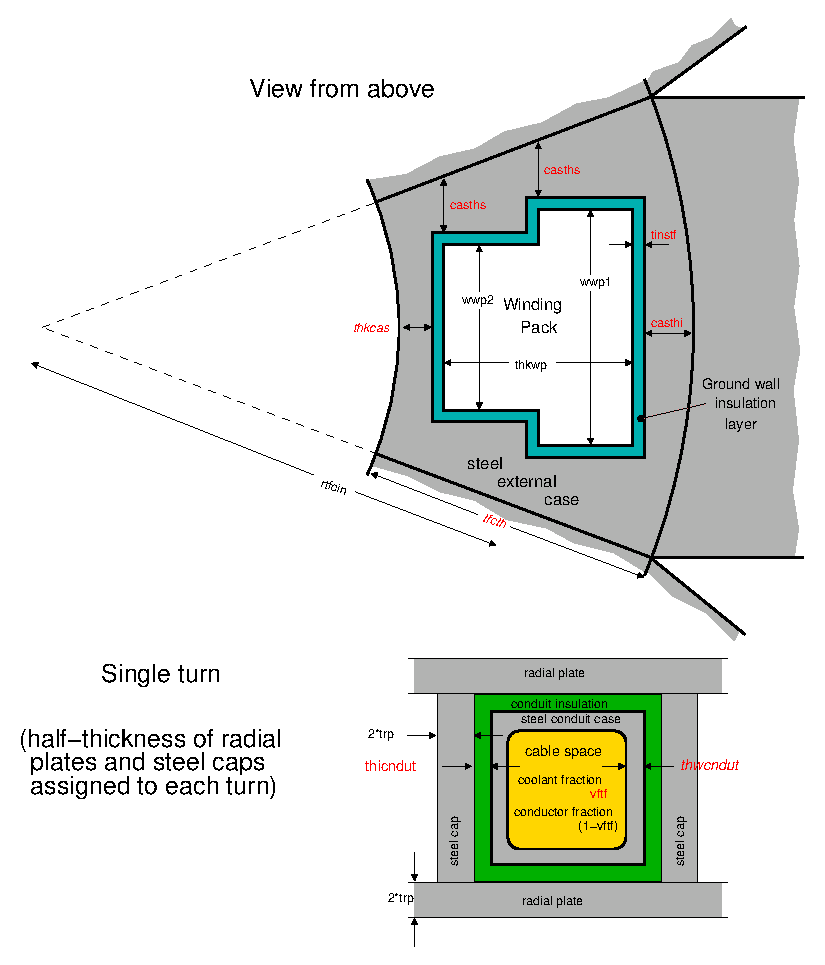
\epsfig{file=tokamak_tfcoil.eps,width=160mm}
\caption[Schematic diagram of the cross-section of a superconducting TF coil
inner leg]
{\label{fig:CICC}
  \textit{Schematic diagram of the cross-section of the inboard leg of a
    superconducting TF coil, showing the CICC (Conductor In Cable Conduit)
    construction. The winding pack contains many turns of cable conduit. The
    cable space contains the superconducting filaments, and circulating liquid
    helium coolant. The variables shown in \Red{red} may be changed by the
    user, and those in italics may be chosen as iteration variables.}
}
\end{figure}

Each TF coil is defined in the $(R,Z)$ plane by four circular arcs of
different radius, which create a D-shaped profile. Because of the finite
number of TF coils used in a tokamak (typically around 16), the toroidal field
has a ripple introduced into it, the amplitude of which can be limited to a
few percent (given by input parameter \texttt{ripmax}, default value 1\%) by
the code by adjusting the outboard gap thickness (labelled \texttt{gapsto} in
Figures~\ref{fig:build_d} and~\ref{fig:build_e}).

Among the TF coil parameters calculated by the code are the maximum allowable
current density, the stresses on the structure, the energy stored and the
magnetic field produced by the coils.

The following options are available within the superconducting TF coil model
(\texttt{itfsup = 1}).

\subsubsection{Superconducting materials}
\label{sec:superconductors}

Switch \texttt{isumattf} specifies which superconducting material is to be
used:
\begin{description}
\item [\texttt{isumattf = 1} :] Nb$_3$Sn superconductor, ITER critical surface
  parameterization~\cite{iter_nb3sn}, standard critical values
\item [\texttt{isumattf = 2} :] Bi-2212 high temperature superconductor %!%!%! ref
\item [\texttt{isumattf = 3} :] NbTi superconductor
\item [\texttt{isumattf = 4} :] Nb$_3$Sn superconductor, ITER critical surface
  parameterization~\cite{iter_nb3sn}, user-defined critical parameters
\end{description}
The fraction of copper present in the superconducting filaments is given by
the value of variable \texttt{fcutfsu} (iteration variable no.\ 59).

For \texttt{isumattf = 2}, a technology adjustment factor \texttt{fhts} may be
used to modify the critical current density fit for the Bi-2212
superconductor, to describe the level of technology assumed (i.e.\ to account
for stress, fatigue, radiation, AC losses, joints or manufacturing variations).
The default value for \texttt{fhts} is 0.5 (a value of 1.0 would be very
optimistic).

For \texttt{isumattf = 4}, important superconductor properties may be input by
the user as follows: the upper critical field at zero temperature and strain
is set using input parameter \texttt{bcritsc}, and the critical temperature at
zero field and strain is set using input parameter \texttt{tcritsc}.

\subsubsection{Current density limits}

The current in the TF coils must be sufficient to produce the required
toroidal field at the centre of the plasma. In tokamaks, the field falls off
at a rate $1/R$, with the peak value occurring at the outer edge of the
inboard portion of the TF coil winding pack ($R_{\mbox{\scriptsize max TF}} =
\mathtt{rbmax}$). The maximum TF coil current depends on the field it produces
and the allowable current density.

\newcommand{\jop}{$J_{\mbox{\scriptsize op}}$ }
\newcommand{\jcrit}{$J_{\mbox{\scriptsize crit}}$}

Three constraints are relevant to the operating current density \jop\ in the
(superconducting) TF coils.

\begin{itemize}

\item To ensure that \jop\ does not exceed the critical value \jcrit, constraint
  equation no.\ 33 should be turned on with iteration variable no.\ 50
  (\texttt{fiooic}).

\item To ensure that \jop\ does not exceed the current density protection limit,
  constraint equation no.\ 35 should be turned on with iteration variable no.\
  53 (\texttt{fjprot}).

\item The critical current density \jcrit\ falls with the temperature of the
  superconductor. The temperature margin $\Delta T$ is the difference between the
  temperature at which \jcrit would be equal to \jop\ and the operating
  temperature. The minimum allowed $\Delta T$ can be set using input parameter
  \texttt{tmargmin} together with constraint equation no.\ 36 and iteration
  variable no.\ 54 (\texttt{ftmargtf}).

  Note that if the temperature margin is positive, \jop\ is guaranteed to be
  lower than \jcrit, and so constraints~33 and~36 need not both be turned on
  (in fact, it is recommended that only one of these two constraints is
  activated in any given run).

\end{itemize}

\subsubsection{Stress model}

Switch \texttt{tfc\_model} controls whether a simple stress model
(\texttt{tfc\_model = 0}, suitable for solid copper TF coils) or a more
complex stress model (\texttt{tfc\_model = 1}) should be used. If
\texttt{tfc\_model = 1}, a two-layer stress model~\cite{Morris_tfc} developed
by CCFE is used.

To enforce the stress limits calculated using either of these models,
constraint equation no.\ 31 (case stress) and/or constraint equation no.\ 32
(conduit stress) should be turned on with iteration variables no.\ 48
(\texttt{fstrcase}) and/or no.\ 49 (\texttt{fstrcond}), respectively. The
stress limit can be adjusted using input parameters \texttt{csutf} and
\texttt{csytf}.

\subsection{Poloidal field coils}
\label{sec:pfcoils}

The poloidal field (PF) coils are used initially to cancel the vertical field
produced at the centre of the plasma by the central solenoid (Section~\ref{sec:ohcoil})
during start-up, and then to maintain the plasma position and shape during the
flat-top period.

\subsubsection{PF coil positions}

The positions and sizes of the PF coils are partly input, and partly
calculated after consideration of the required currents and allowable current
density.

The PF coil locations are controlled using a set of switches stored in array
\texttt{ipfloc} (see Figure~\ref{fig:build_d}), and are calculated in routine
\texttt{PFCOIL}. The coils are (usually) organised into groups containing two
PF coils placed symmetrically above and below the midplane, and each group
\texttt{j} has an element \texttt{ipfloc(j)} assigned to it. Input parameter
\texttt{ngrp} should be set to the number of groups, and \texttt{ncls(j)}
should be assigned the number of coils in each group --- which should be
\texttt{2} in each case.

In the following, all variables are defined in the variable descriptor file
\texttt{vardes.html}. The values for \texttt{rpf1}, \texttt{rpf2},
\texttt{zref(j)} and \texttt{routr} should be adjusted by the user to locate
the PF coils accurately.

The three possible values of \texttt{ipfloc(j)} correspond to the following PF
coil positions: (\Red{Redo taking into account snull and other recent changes
  e.g. rclsnorm})

\begin{description} %!%!%! check this

\item [\texttt{ipfloc(j) = 1} :]  PF coils are placed above the central solenoid (one
group only);
\begin{eqnarray*}
R & = & \mathtt{rohc + rpf1} \\
Z & = & \pm
\mathtt{( hmax*ohhghf + 0.1 + 0.5*( hmax*(1.0D0-ohhghf)+tfcth+0.1) )}
\end{eqnarray*}

\item [\texttt{ipfloc(j) = 2} :]  PF coils are placed above the TF coils (one
group only);
\begin{eqnarray*}
R & = & \mathtt{rmajor + rpf2*triang*rminor} \hspace{62mm} \\
Z & = & \pm (\mathtt{hmax + tfcth + 0.86})
\end{eqnarray*}

\item [\texttt{ipfloc(j) = 3} :]  PF coils are placed radially outside the TF
coils (any number of groups \Red{(?)});
\begin{eqnarray*}
R & = & \mathtt{rtot + tfthko/2.0D0 + routr} \hspace{63mm}\\
Z & = & \pm(\mathtt{rminor*zref(j)})
\end{eqnarray*}

\end{description}

The void fraction (for coolant) in each coil \texttt{i}'s winding pack is
given by \texttt{vf(i)}.

\subsubsection{PF coil currents}

The peak current per turn, \texttt{cptdin(i)}, and the winding pack peak
current density \texttt{rjconpf(i)} in each PF coil \texttt{i} are inputs. The
PF coil currents vary as a function of time during the tokamak operation as
indicated in Figure~\ref{fig:current_vs_time}. They contribute part of the
flux swing necessary to maintain the plasma current (see
Section~\ref{sec:ohcoil}).

\begin{figure}[tbph]
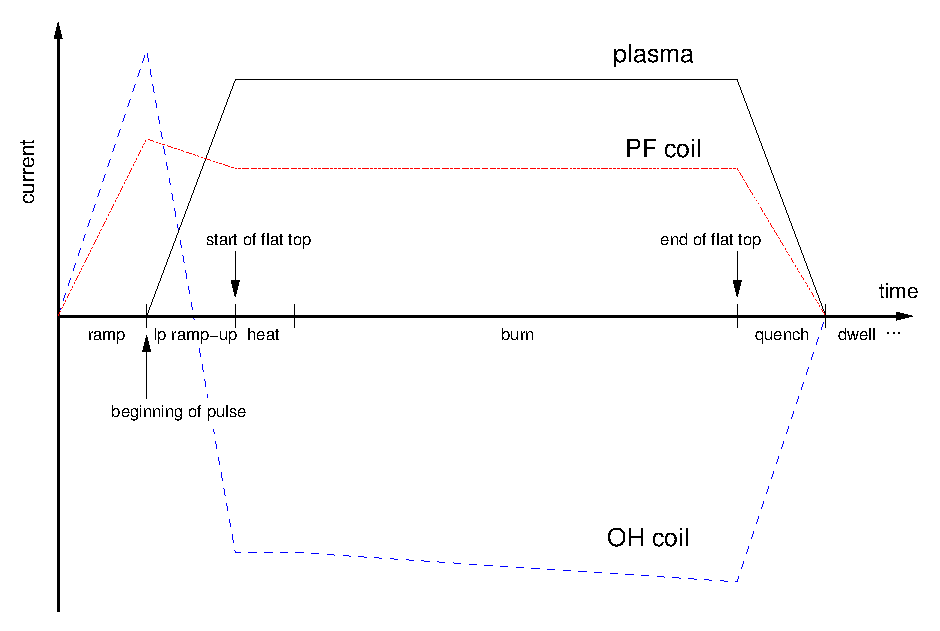
\epsfig{file=current_vs_time.eps,width=170mm}
\caption[Coil and plasma current waveforms]
{\label{fig:current_vs_time}
  \textit{Plot showing schematically the current waveforms for the plasma, a
    typical PF coil, and the central solenoid. Note that the currents in some
    of the PF coils may be the opposite sign to that shown, and the central
    solenoid current may remain positive during the $I_p$ ramp-up period,
    although it will pass through zero during the burn phase.}
}
\end{figure}

\subsubsection{PF coil resistance}

The PF coils can be either resistive or superconducting. This is determined
from the value of \texttt{ipfres}. If \texttt{ipfres = 0}, the PF coils and
the central solenoid are assumed to be superconducting. If \texttt{ipfres = 1},
they are assumed to be resistive, with their resistivity given by the value of
variable \texttt{pfclres}.

\subsubsection{Superconducting materials}

If \texttt{ipfres = 0}, switch \texttt{isumatpf} specifies which
superconducting material is to be used for the PF coils. The values for
\texttt{isumatpf} are used in the same way as switch \texttt{isumattf} is for
the TF coils (see Section~\ref{sec:superconductors}).

The fraction of copper present in the superconducting filaments is given by
the value of variable \texttt{fcupfsu}.

If the PF coils are superconducting, a steel case is assumed to surround the
current-carrying winding pack to take the hoop stress. Its cross-sectional
area is determined by the $J \times B$ hoop force on the coil divided by the
allowable hoop stress, given by input parameter \texttt{sigpfcalw}. The input
parameter \texttt{sigpfcf} provides a scale factor (default is 0.666) to
adjust the hoop force if required, to indicate what proportion of the force is
supported by the case.

\subsection{Central solenoid}
\label{sec:ohcoil}

Formerly known as the ohmic heating (OH) coil, the central solenoid is a PF
coil used primarily during start-up (but also during the burn phase) to create
and maintain the plasma current by inductive means. Swinging (changing) the
current through the central solenoid causes a change in the flux linked to the
plasma region, inducing a current in it. \process\ calculates the amount of
flux required to produce the plasma current, and also the amount actually
available. The code measures the magnetic flux in units of Volt-seconds ($=$
Webers).

Switch \texttt{iohcl} controls whether a central solenoid is present. A value
of \texttt{1} denotes that this coil is present, and should be assigned a
non-zero thickness \texttt{ohcth}. A value of \texttt{iohcl = 0} denotes that
no central solenoid is present, in which case the thickness \texttt{ohcth}
should be set to zero. No PF coils should be located at positions defined by
\texttt{ipfloc(j) = 1} if no central solenoid is present.

The central solenoid can be either resistive or superconducting (controlled
via switch \texttt{ipfres} as for the other PF coils), and if superconducting,
switch \texttt{isumatoh} determines the superconducting material to use ---
its value is used like \texttt{isumattf} and \texttt{isumatpf}. The fraction
of copper present in the superconducting filaments is given by the value of
variable \texttt{fcuohsu}.

If the central solenoid is superconducting, the coil contains steel for
strength. The cross-sectional area of steel is determined by the $J \times B$
hoop force on the coil divided by the allowable hoop stress, calculated as the
lower of the two quantities (2/3 * \texttt{csytf}) and (0.5 * \texttt{csutf}),
where input parameter \texttt{csytf} (Pa) is the yield strength of the steel,
and \texttt{csutf} (Pa) is the ultimate strength of the steel. (This is the
same calculation as for the allowable stress in the TF coil cases.) A steel
thickness is given in the output, which would be the thickness of a
steel case of the same cross-sectional area if it simply surrounded the
conducting region.

\subsubsection{Current density inputs and limits}

The (absolute value of the) central solenoid current density at the
end-of-flat-top (`EOF'), \texttt{coheof} is specified by the user, and can be
used as an iteration variable (no.\ 37). The current density at the
beginning-of-pulse (`BOP' --- see Figure~\ref{fig:current_vs_time}) is
specified as a (positive) fraction of \texttt{coheof} using \texttt{fcohbop}
(iteration variable no.\ 41). The current density in the CS at all other times
is calculated by taking account of the flux swing necessary to initiate and
maintain the plasma current. The positive or negative sign of the current at
each time is calculated automatically.

The current density in the central solenoid can be limited at the BOP and at
the EOF. To limit the current density at the BOP, constraint equation no.\ 27
should be turned on with iteration variable no.\ 39 (\texttt{fjohc0}). To
limit the current density at the EOF, constraint equation no.\ 26 should be
turned on with iteration variable no.\ 38 (\texttt{fjohc}).

As for the TF coils, the critical current density \jcrit\ falls with the
temperature of the superconductor. The temperature margin $\Delta T$ is the
difference between the temperature at which \jcrit would be equal to \jop\ and
the operating temperature. The minimum allowed $\Delta T$ can be set using
input parameter \texttt{tmargmin} together with constraint equation no.\ 60
and iteration variable no.\ 106 (\texttt{ftmargoh}).

Note that if the temperature margin is positive, \jop\ is guaranteed to be
lower than \jcrit, and so constraints~26, 27 and~60 need not all be turned on
(in fact, it is recommended that EITHER the latter constraint, OR the former
two constraints, is/are activated in any given run).

\subsubsection{Plasma current ramp-up time}
\label{sec:tohs}

In the steady-state power plant scenario ($\mathtt{lpulse \not= 1}$ --- see
Section~\ref{sec:pulsed}), the length of time taken for the central solenoid
current to (possibly) reverse (which is equal to the plasma current ramp-up time --- see
Figure~\ref{fig:current_vs_time}) is determined from the value of switch
\texttt{tohsin}. If \texttt{tohsin = 0.0D0}, then the plasma current ramp-up
time \texttt{tohs} in seconds is given by $\mathtt{tohs} = I_p / 0.5$, where
$I_p$ is the plasma current in MA\@. Furthermore, the PF coil ramp time
\texttt{tramp} and shutdown time \texttt{tqnch} are set equal to
\texttt{tohs}.  If $\mathtt{tohsin \not= 0.0D0}$, the plasma current ramp-up
time \texttt{tohs = tohsin}, and the PF coil ramp and shutdown times are input
parameters.

If, however, a pulsed power plant is being modelled (\texttt{lpulse = 1}), the
plasma current ramp-up time \texttt{tohs} is either an input parameter, or it can be
iterated by using iteration variable~65. The ramp and shutdown times in the
pulsed case are always set equal to \texttt{tohs}. To ensure that the plasma
current ramp rate during start-up is prevented from being too high, as
governed by the requirement to maintain plasma stability in $l_i$-$q_\psi$
space, constraint equation no.\ 41 should be turned on with iteration variable
no.\ 66 (\texttt{ftohs}).

\subsection{Auxiliary power systems: heating and current drive}
\label{sec:hcd}

\subsubsection{Current Drive}

The use of purely inductive current drive leads to pulsed plant operation
because of the limited flux swing that can be achieved using the central
solenoid. This poses problems due to the fact that fatigue failures may
result, and there would also be a need for thermal storage to maintain a level
supply between pulses. However, the plasma current can also be produced and
maintained (partially or wholly) using non-inductive means which, in
principle, removes this restriction. \process\ contains a number of auxiliary
current drive schemes, including various RF methods (Lower Hybrid, Electron
Cyclotron, and Ion Cyclotron (Fast Wave) current drives) and also Neutral Beam
current drive systems. The code calculates the efficiency and the resulting
power requirements of the chosen system.

The fraction of the required plasma current to be produced by non-inductive
means, \texttt{fvsbrnni}, should be set, and flag \texttt{irfcd} should be set
to \texttt{0} for purely inductive scenarios, or \texttt{1} otherwise. The
current drive efficiency model to be used in this latter case is defined by
the value of switch \texttt{iefrf}:-

\begin{description}
\item [\texttt{iefrf = 1} :] Fenstermacher Lower Hybrid model
\item [\texttt{iefrf = 2} :] Ion cyclotron model~\cite{IPDG}
\item [\texttt{iefrf = 3} :] Fenstermacher electron cyclotron resonance model
\item [\texttt{iefrf = 4} :] Ehst Lower Hybrid model
\item [\texttt{iefrf = 5} :] ITER neutral beam model~\cite{IPDG,172}
\item [\texttt{iefrf = 6} :] Culham Lower Hybrid model~\cite{172}
\item [\texttt{iefrf = 7} :] Culham electron cyclotron model~\cite{172}
\item [\texttt{iefrf = 8} :] Culham neutral beam model~\cite{172}
\item [\texttt{iefrf = 9} :] Oscillating Field current drive (RFPs only --- see
Section~\ref{sec:rfpcd})
\end{description}

(Note that, at present, the neutral beam models assume parabolic plasma
profiles only.)

It is sometimes useful to adjust artificially the current drive efficiency
values produced by these routines. This can be achieved by setting the scaling
coefficient \texttt{feffcd}. The wall plug to plasma efficiencies can also be
adjusted, by changing the relevant variable (\texttt{etaech}, \texttt{etalh},
\texttt{etanbi} or \texttt{etaof}).

\subsubsection{Plasma heating}

In addition to current drive, some auxiliary power can be used purely to heat
the plasma. The value of input parameter \texttt{pheat} determines the amount
of auxiliary \textit{heating}\/ power (in Watts) to be applied to the
plasma. This variable may be used as an iteration variable (no.\ 11).

\subsubsection{Neutral beam access}

If present, a neutral beam injection system needs sufficient space between the
TF coils to be able to intercept the plasma tangentially. The major radius
\texttt{rtanbeam} at which the centreline of the beam is tangential to the
toroidal direction is user-defined using input parameter \texttt{frbeam},
which is the ratio of \texttt{rtanbeam} to the plasma major radius
\texttt{rmajor}. The maximum possible tangency radius \texttt{rtanmax} is
determined by the geometry of the TF coils --- see Figure~\ref{fig:portsize},
and this can be enforced using constraint equation no.\ 20 with iteration
variable no.\ 33 (\texttt{fportsz}). The thickness of the beam duct walls may
be set using input parameter \texttt{nbshield}.

\begin{figure}[tbph]
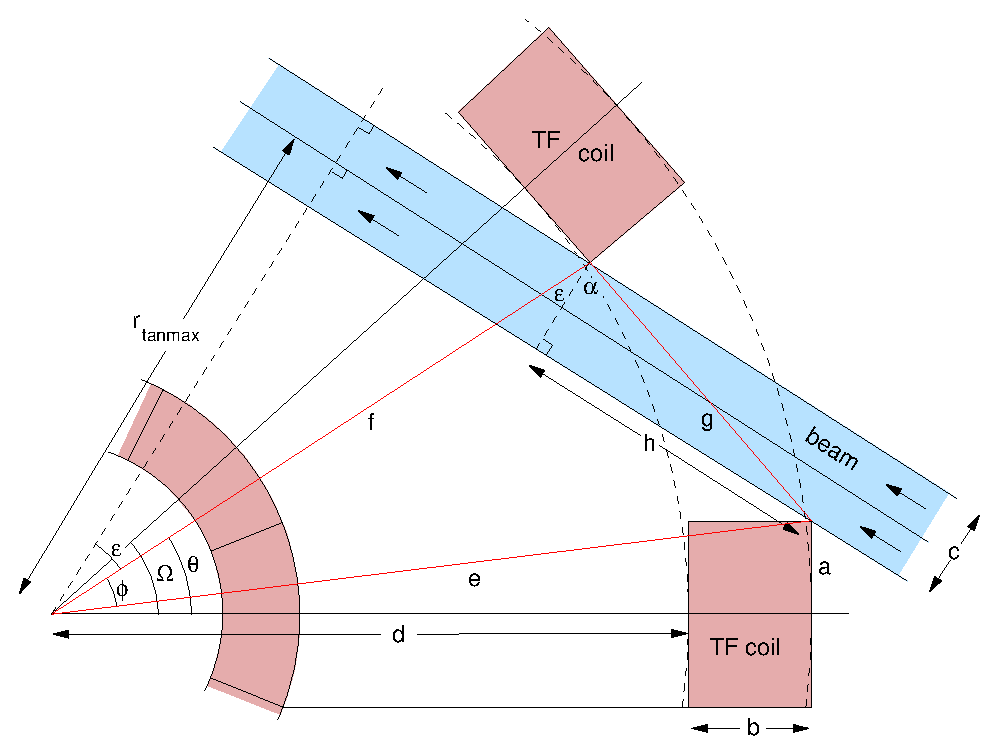
\epsfig{file=portsize.eps,width=160mm}
\caption[Schematic diagram of the neutral beam access geometry]
{\label{fig:portsize}
  \textit{Top-down schematic view of the neutral beam access geometry. The beam
    with the maximum possible tangency radius is shown here.}
}
\end{figure}

\subsubsection{Neutral beam losses}

Input parameter \texttt{forbitloss} can be used to specify the fraction of the
net injected neutral beam power that is lost between the beam particles'
ionisation and thermalisation (i.e.\ the orbit loss fraction). The power lost
is assumed to be absorbed by the first wall.

There are two constraint equations that can be used to control the beam
penetration and deposition, as follows:

\begin{itemize}

\item It is necessary to use a beam energy that simultaneously gives adequate
  penetration of the beam to the centre of the plasma and tolerable
  shine-through of the beam on the wall after the beam has traversed the
  plasma. The number of exponential decay lengths, $\tau$, for the beam power
  to fall before it reaches the plasma centre should be in the region of $\sim
  4$--6~\cite[Section 4.3.2]{172}. Constraint equation no.\ 14 may be used to
  force $\tau$ to be equal to the value given by input parameter
  \texttt{tbeamin}, and is therefore in effect a beam energy consistency
  equation.

\item Alternatively, constraint equation no.\ 59 with iteration variable no.\
  105 (\texttt{fnbshinef}) may be used to ensure that the beam power fraction
  emerging from the plasma is no more than the value given by input parameter
  \texttt{nbshinefmax}.

\end{itemize}

It is recommended that \textbf{only one} of these two constraint equations is
used during a run.

\subsubsection{Ignited plasma}
\label{sec:ignited}

Switch \texttt{ignite} can be used to denote whether the plasma is ignited,
i.e.\ fully self-sustaining without the need for any injected auxiliary power
during the burn. If \texttt{ignite = 1}, the calculated injected power does
not contribute to the plasma power balance (Section~\ref{sec:corepower}),
although the cost of the auxiliary power system is taken into account (the
system is then assumed to be required to provide heating etc.\ during the
plasma start-up phase only --- use \texttt{pheat} to indicate the power
requirement). If \texttt{ignite = 0}, the plasma is not ignited, and the
auxiliary power is taken into account in the plasma power balance during the
burn phase. Also, constraint equation no.\ 28 can be turned on to enforce the
fusion gain $Q$ to be at least \texttt{bigqmin}.

\subsection{Structural components}

Structural components are required to provide support for the fusion power
core systems against gravity and the magnetic forces that will be encountered
during operation. The required structural masses and their costs are
calculated.

\subsection{Cryostat and vacuum system}

The internal vacuum vessel provides a toroidal evacuated chamber containing
the plasma, first wall, blanket and shield, and the space between this item
and the external cylindrical cryostat encloses those components that need to
operate at liquid helium temperatures. These include any superconducting (TF
or PF) coils and the inter-coil structure. \process\ calculates the cryogenic
power load and the resulting heat exchanger requirements.

The vertical distance \textit{h}\/ between the uppermost PF coil and the
external cryostat lid may be adjusted by changing the value of input parameter
\texttt{clhsf}; a scaling based on ITER is used:
\begin{equation}
h = \mathtt{clhsf} \, \left( \frac{2 \times \mathtt{rdewex}}{28.440} \right)
\end{equation}

The vacuum system is used for four different processes. Firstly, before plasma
operations the chamber must be evacuated to remove outgassed impurities from
the structure. Secondly, the chamber must be re-evacuated between burn
operations. Thirdly, helium ash must be removed to prevent it from diluting
the fuel. Finally, deuterium and tritium is removed on a steady state
basis. \process\ calculates the parameters of a vacuum system that satisfy
all four requirements, with the option of either turbo pumps or cryo pumps
being used.

Switch \texttt{ntype} controls whether a turbopump (\texttt{ntype = 0}) or a
cryopump (\texttt{ntype = 1}) is used in the vacuum system.

\subsection{Power conversion and heat dissipation systems}
\label{sec:powerflow}

The \process\ power plant takes into account all the systems required to
perform the necessary conversion of fusion power to electricity, from the
coolant systems in the plant components to the heat exchangers and turbines.
%Figure~\ref{fig:pwrconv} shows schematically the overall power transfer
%mechanisms used by the code.
%
%\begin{figure}[tbph]
%\centerline{\epsfig{file=PWR.ps,width=160mm,height=160mm,
%bbllx=0mm,bburx=200mm,bblly=0mm,bbury=200mm,clip=}}
%\vspace{-12mm}
%\caption[Power conversion mechanisms within \process]
%{\label{fig:pwrconv}
%  \textit{Schematic diagram showing the power conversion mechanisms used in
%    \process \cite[Note 0166]{PWF}.}
%}
%\end{figure}
%
%Many of the power conversion efficiencies shown in Figure~\ref{fig:pwrconv}
%can be adjusted by the user.

Figures~\ref{fig:powerflow2} and \ref{fig:powerflow3} show schematically the
overall power transfer mechanisms within the power plant outside of the plasma
(the power flow \textit{within}\/ the plasma is shown in
Figure~\ref{fig:powerflow1}).

(Note that these figures and the following description assume that switch
\texttt{ipowerflow} is set to 1; its default value is currently
zero, as the new power flow model is in draft form.)

\begin{figure}[tbph]
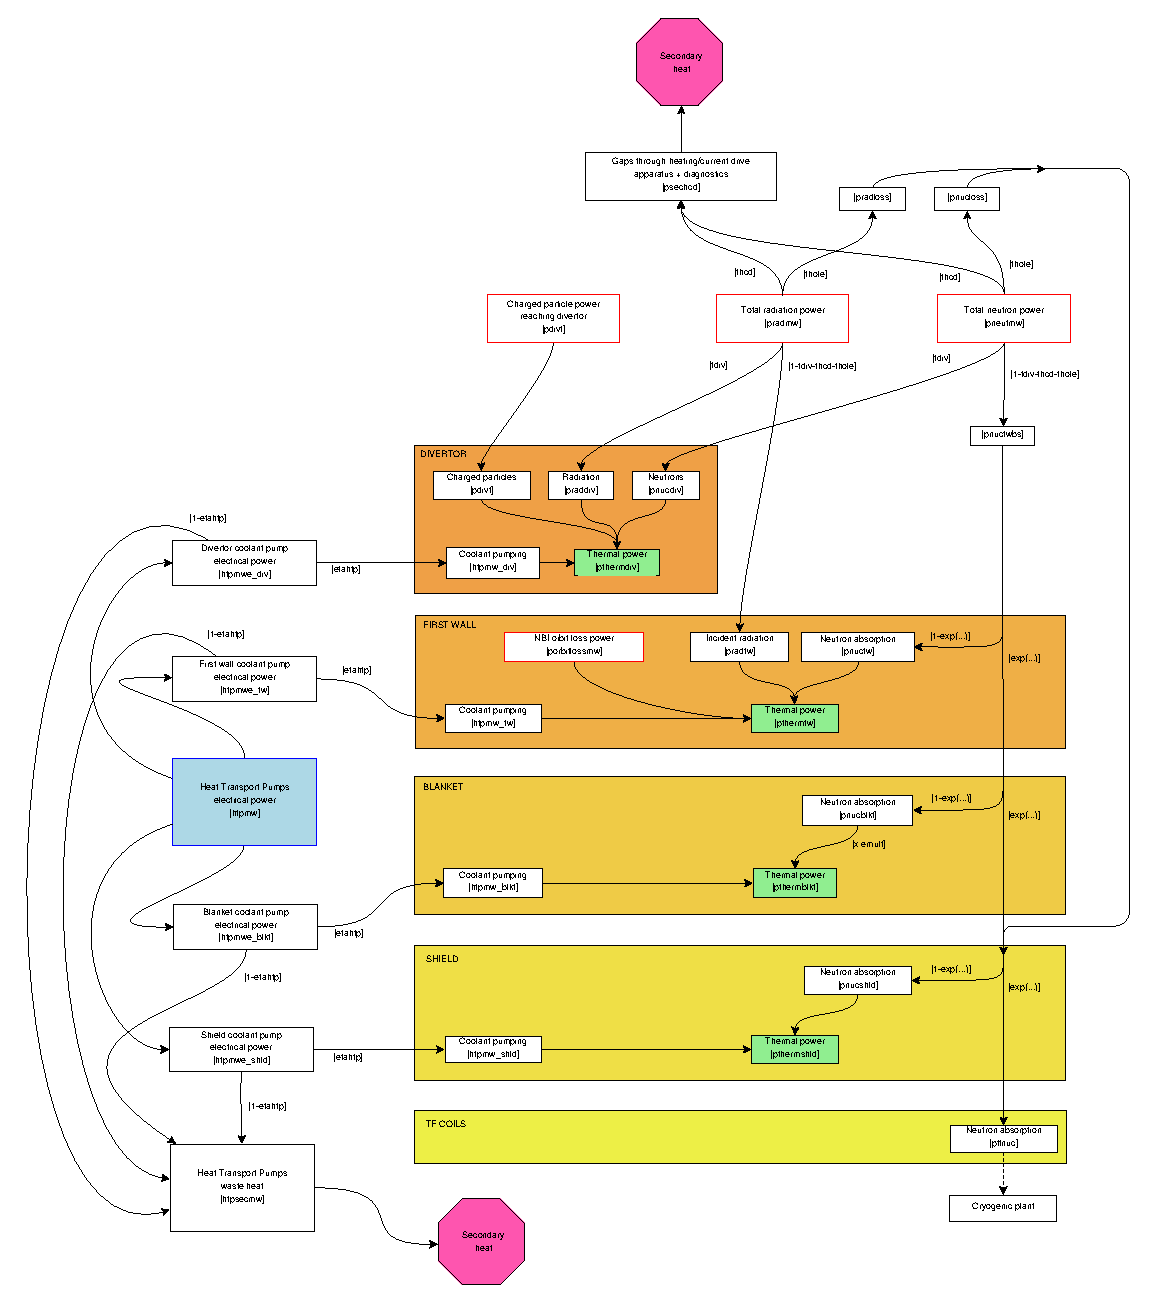
\epsfig{file=powerflow2.eps,width=170mm}
\caption[Power flow within the fusion power plant core]
{\label{fig:powerflow2} \textit{Schematic diagram of the flow of power from
    the plasma to the thermal power deposited within the divertor, first wall,
    blanket and shield. Variable names are given in [\ldots]. The three
    red-bordered contributions are passed from Figure~\ref{fig:powerflow1},
    while the blue box comes from Figure~\ref{fig:powerflow3}.} }
\end{figure}

Figure~\ref{fig:powerflow2} shows how the power contributions originating from
the plasma are converted to thermal power in the first wall, blanket, shield
and divertor.

The radiation and neutron power contributions are distributed according to the
following area fractions of a theoretical first wall with 100\% coverage,
which may be set as input parameters: \texttt{fdiv} (divertor area fraction),
\texttt{fhcd} (heating / current drive / diagnostics apparatus), and
\texttt{fhole} (any other gaps). The remaining fraction
(\texttt{1-fdiv-fhcd-fhole}) is the area fraction of the actual first wall.

\subsubsection{Divertor}

All of the charged particle transport power leaving the plasma is assumed to
be absorbed in the divertor, along with a proportion \texttt{fdiv} of the
radiation power and the neutron power. The power necessary to drive the
divertor coolant pumps $P$ (= \texttt{htpmw\_div} in
Figure~\ref{fig:powerflow2}) is assumed to be a fraction $f$ (= input
parameter \texttt{fpumpdiv}) of the total thermal power absorbed by the
divertor, which includes the coolant pump power itself:
\begin{eqnarray*}
P & = & f . (\mathtt{pdivt} + \mathtt{praddiv} + \mathtt{pnucdiv} + P) \\
\Longrightarrow P & = & \frac{f}{1-f} . (\mathtt{pdivt} + \mathtt{praddiv} +
\mathtt{pnucdiv})
\end{eqnarray*}
The efficiency of the divertor coolant pump is given by input parameter
\texttt{etahtpdiv}.

Switch \texttt{iprimdiv} may be used to specify whether the thermal power
deposited in the divertor becomes primary (high-grade) thermal power
(\texttt{iprimdiv = 1}) or secondary (low-grade) thermal power (see
Figure~\ref{fig:powerflow3}).

\subsubsection{First wall}

All of the remaining radiation power (i.e.\ the fraction not incident upon the
divertor or lost through holes or the heating / current drive apparatus) is
assumed to be absorbed by the first wall. The same fraction of the neutron
power is assumed to pass into the first wall. Of this neutron power, a
fraction $(1-e^{\lambda/d})$ is assumed to be absorbed in the first wall
(of thickness $d$), given by the neutron decay length $\lambda$ in the first wall
(input parameter \texttt{declfw}).

As for the divertor, the first wall coolant pump power is a fraction
\texttt{fpumpfw} of the total thermal power absorbed by the first wall, and
the efficiency of the first wall coolant pump is \texttt{etahtpfw}.

\subsubsection{Blanket}

A fraction (\texttt{1 - exp(declblkt/blnkoth)}) of the neutron power incident
on the blanket is assumed to be absorbed in the blanket, where input parameter
\texttt{declblkt} is the neutron decay length in the blanket. This absorbed
neutron power is multiplied by the energy multiplication factor \texttt{emult}
to calculate its contribution to the thermal power within the blanket.

As for the other components, the blanket coolant pump power is a fraction
\texttt{fpumpblkt} of the total thermal power absorbed by the blanket, and
the efficiency of the blanket coolant pump is \texttt{etahtpblkt}.

\subsubsection{Shield}

A fraction (\texttt{1 - exp(declshld/shldoth)}) of the neutron power incident
on the shield is assumed to be absorbed in the shield, where input parameter
\texttt{declshld} is the neutron decay length in the shield.

As for the other components, the shield coolant pump power is a fraction
\texttt{fpumpshld} of the total thermal power absorbed by the shield, and
the efficiency of the shield coolant pump is \texttt{etahtpshld}.

Switch \texttt{iprimshld} may be used to specify whether the thermal power
deposited in the shield becomes primary (high-grade) thermal power
(\texttt{iprimshld = 1}) or secondary (low-grade) thermal power (see
Figure~\ref{fig:powerflow3}).

The remaining neutron power after passing through the shield is assumed to be
absorbed in the TF coils as quantity \texttt{ptfnuc}. This power contributes
to the total cryogenic power requirements of the machine.

\subsubsection{Power conversion outside of the fusion power core}

Figure~\ref{fig:powerflow3} summarises the power conversion mechanisms outside
of the fusion power core.

\begin{figure}[tbph]
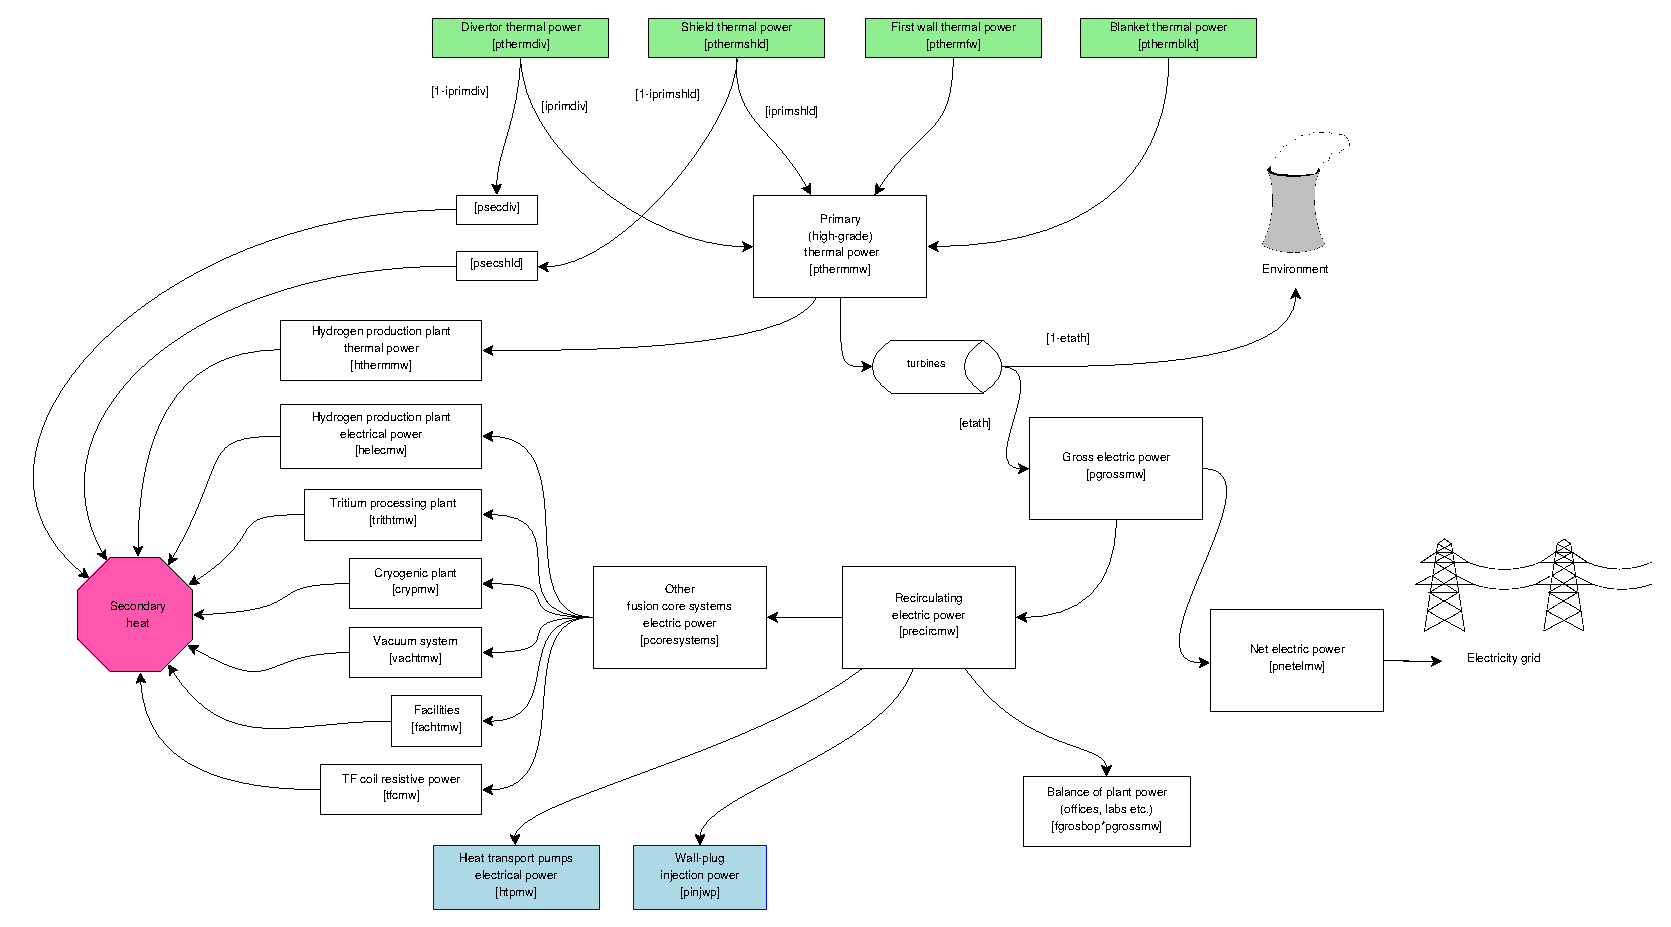
\epsfig{file=powerflow3.eps,width=170mm}
\caption[Power flow outside the fusion power plant core]
{\label{fig:powerflow3} \textit{Schematic diagram of the flow of power beyond
    the fusion power core, showing the origin of the primary and secondary
    thermal power and the electrical power balance within the plant. Variable
    names are given in [\ldots]. The input power contributions in green boxes
    originate in Figure~\ref{fig:powerflow2}. }  }
\end{figure}

The primary (high-grade, i.e.\ useable) thermal power comprises the thermal
power contributions from the first wall and blanket, and possibly also those
from the divertor and shield, depending on the values of the switches
\texttt{iprimdiv} and \texttt{iprimshld} as described in the previous
sections. The primary thermal power (less any thermal power required to
produce hydrogen in a hydrogen production plant --- see
Section~\ref{sec:hplant}) is used to produce steam to turn the turbines, thus
generating the plant's gross electrical power, with an efficiency given by
input parameter \texttt{etath}. The power lost via the turbines' inefficiency
escapes from the plant to the environment.

The electrical power required to operate the power plant itself is the
so-called recirculating electric power. Any surplus is exported to the
electricity grid as net electric power.

The recirculating power comprises the electrical power required to run all of
the associated electrical systems surrounding the fusion power core, plus the
on-site building services, offices, etc., as shown in
Figure~\ref{fig:powerflow3}. Of these, the cryogenic plant power includes the
power required to cool the TF coils from the neutron power absorbed by the
coils, the PF coils (as defined by the ratio of the total PF coil stored
energy to the fusion power pulse time \texttt{tpulse}), and other `cold'
components.

\subsection{Buildings}

The volume and ground area of all the various buildings on a power plant site
are included in the \process\ calculations for the benefit of the costing
algorithms. %!%!%! expand

\section{Spherical Tokamak Model}
\label{sec:tart}

\process\ has the ability to perform studies on tokamaks in the low aspect ratio
regime (major radius $\leq 2 \times$ minor radius). The physics and
engineering issues~\cite{tart} associated with these machines are somewhat
different from those of conventional aspect ratio, and this is reflected by
the following special models~\cite{storac} in \process.

\begin{enumerate}

\item The inboard build of a spherical tokamak (ST) is very different from
  that in a conventional tokamak. There is no inboard blanket (and possibly no
  inboard shield), and the inboard TF coil legs are replaced by a single
  centrepost. The radial build is altered so that, starting from the
  centreline ($R = 0$), the component order is: TF coil, gap, central
  solenoid, vacuum vessel, and then continuing as in Figure~\ref{fig:build_d}
  (a D-shaped cross-section is assumed for the first wall, blanket, shield and
  vacuum vessel).

\item Spherical tokamaks have resistive TF coils that combine into a single
  centrepost at the centre of the machine. The centrepost is constructed from
  copper (as are the outboard TF coil sections), and is tapered lengthways so
  that it is narrowest at the midplane of the device.  Routine
  \texttt{CNTRPST} calculates various parameters relevant to the centrepost,
  including the pump pressure, maximum temperature and pipe radius, and these
  may be limited using constraint equations~43 to~46 if required:

  \begin{itemize}
  \item Equation~43 is a consistency equation for the average centrepost
    temperature.
  \item Equation~44 can be used to limit the peak centrepost temperature to a
    maximum value (\texttt{ptempalw}) using iteration variable no.\ 68
    (\texttt{fptemp}).
  \item Equation~45 can be used to force a lower limit to the edge safety
    factor $q_{lim}$ (see below), using iteration variable no.\ 71 (\texttt{fq}).
  \item Equation~46 can be used to apply an upper limit to the ratio of plasma
    current to TF coil (``rod'') current, using iteration variable no.\ 72
    (\texttt{fipir}).
  \end{itemize}

\item A gaseous divertor model is used, and a simple divertor heat load
  calculation is employed, rather than the more complex divertor model assumed
  for conventional aspect ratio tokamaks.

\item A simple PF coil current scaling algorithm is available for use with the
  ST option.

\item The plasma shaping terms (elongation and triangularity) can be
  calculated directly given the aspect ratio, using \texttt{ishape = 1} (see
  Section~\ref{sec:plasma_geometry}). This setting also scales the lower
  limit~\cite{storac} for the edge safety factor, for use with constraint
  equation no.\ 45:
  \begin{equation}
    q_{lim} = 3 \, (1 + 2.6*\epsilon^{2.8})
  \end{equation}
  where $\epsilon = a/R$. 

\item Among the physics models that differ from those relevant to conventional
  aspect ratio machines are (i) the plasma poloidal field $B_{pol}$, (ii) the
  bootstrap current fraction, (iii) the beta limit, and (iv) the neutron
  heating of the centrepost~\cite{storac}.

\end{enumerate}

\subsection{Spherical tokamak switches}

Switch \texttt{itart} provides overall control of the ST switches within the
code, and subroutine \texttt{CHECK} ensures that no conflicting values are
inadvertently set by the user in the input file. Table~\ref{tab:tart}
summarises the switch values relevant to each aspect ratio regime.
\begin{table}[tbph]
\begin{center}
  \begin{tabular}{||l|c|c||} \hline
    & conventional aspect ratio & low aspect ratio \\
    switch & \texttt{itart = 0} & \texttt{itart = 1} \\ \hline
    \texttt{ishape} & 0, 2 & 0, 1 \\
    \texttt{ibss} (Section~\ref{sec:bootstrap}) & 1, 2, 3 & 2, 3 \\
    \texttt{icurr} (Section~\ref{sec:current_scaling}) & 1, 3, 4, 5, 6, 7 & 2 \\
    \texttt{itfsup} (Section~\ref{sec:tfcoil}) & 0, 1 & 0 \\
    \hline
\end{tabular}
\end{center}
\caption[\process\ switches for spherical tokamaks]
{\label{tab:tart}
  \textit{Summary of the switch values in PROCESS that relate to
    conventional aspect ratio and low aspect ratio machines.}
}
\end{table}

\section{Pulsed Plant Operation}
\label{sec:pulsed}

If the plasma current is not to be driven by purely non-inductive means, it is
necessary to operate the plant in a pulsed manner as the current swing in the
OH/PF coils cannot be continued indefinitely. \process\ can perform a number of
calculations relevant to a pulsed power plant, as detailed below.

Switch \texttt{lpulse} determines whether the power plant is assumed to be
based on steady-state (\texttt{lpulse = 0}) or pulsed (\texttt{lpulse = 1})
operation.

\subsection{Thermal cycling package}

This performs calculations on the first wall of the machine. Evaluation of the
mechanical and thermal stresses on this component lead to a measure of the
maximum number of cycles to which the first wall can be subjected, and hence
to the minimum allowable length of each reactor cycle for a specified first
wall lifetime. The cycle time can be constrained to be at least the minimum
value by turning on constraint equation no.\ 42 with iteration variable no.\
67 (\texttt{ftcycl}).

The thickness of the first wall is constrained to lie within lower and upper
bounds, which ensures that it can withstand the internal coolant pressure and
the peak temperature and neutron fluence.

Switch \texttt{itcycl} activates the desired model for the first wall axial
stress calculations. If \texttt{itcycl = 1} (the default), the wall is fully
constrained axially, and no bending can occur. If \texttt{itcycl = 2}, there
is no constraint on the axial motion, but no bending can occur. Finally, if
\texttt{itcycl = 3}, again there is no axial constraint, and bending is
allowed to occur.

\subsection{First wall coolant temperature rise limit}

The rise in temperature of the first wall coolant can be limited to be no more
than the value of \texttt{dtmpmx} by turning on constraint equation no.\ 38 with
iteration variable no.\ 62 (\texttt{fdtmp}).

\subsection{First wall peak temperature limit}

The maximum first wall temperature can be limited to be no more than the value
of variable \texttt{tpkmax} by turning on constraint equation no.\ 39 with
iteration variable no.\ 63 (\texttt{ftpeak}).

\subsection{Start-up power requirements}

The minimum auxiliary power required during the start-up (ignition) phase is
calculated on the basis of a POPCON analysis. Ignition is accessed via the
so-called Cordey Pass (the path in plasma density--temperature space which
minimises the power requirement) and the code ensures that there is sufficient
auxiliary power to accommodate this. In fact, this calculation is very
CPU-intensive, so the relevant routine is not called at present. In practice,
the auxiliary power tends to exceed the minimum allowable value anyway,
without any need to constrain it to do so.

The auxiliary power reaching the plasma can be forced to be more than the
minimum allowable value \texttt{auxmin} by turning on constraint equation no.\
40 with iteration variable no.\ 64 (\texttt{fauxmn}). The value of
\texttt{auxmin} is determined by the code if the start-up model is activated,
otherwise it may be initialised via the input file.

\subsection{Plasma current ramp-up time}

This calculation ensures that the plasma current ramp rate during start-up is
prevented from being too high, as governed by the requirement to maintain
plasma stability in $l_i$ - $q_\psi$ space (see Section~\ref{sec:tohs}).

\subsection{Burn time}

The length of the burn time is calculated from the surplus volt-seconds
available from the OH/PF coil system during the plasma burn phase, after the
flux required during the plasma start-up is taken into account. A minimum burn
time can be enforced via constraint equation no.\ 13 and iteration variable
no.\ 21 (\texttt{ftburn}).

\subsection{Thermal storage}

During every cycle there is a period when no fusion power is produced. The net
electric output from the plant must, however, be maintained, and this is
achieved using thermal storage. There are three types of thermal storage
available within \process, and the value of switch \texttt{istore} determines
which is to be used. If \texttt{istore = 1} (the default), option~1 of
Ref.~\cite{ELECTROWATT} is assumed, which utilises the thermal storage
inherent in the machine's steam cycle equipment. This should be used if the
machine down time is less than 100~seconds. If \texttt{istore = 2}, option~2
of Ref.~\cite{ELECTROWATT} is assumed, which uses the same method as before,
but augments it with an additional boiler. This may be used for machine down
times of up to 300~seconds. Finally, if \texttt{istore = 3}, a large stainless
steel block acts as the thermal storage medium.

\section{Hydrogen Production Facility}
\label{sec:hplant}

Fusion power plants have been mooted as a means of producing hydrogen for use
in fuel cells for cars, for instance. \process\ includes options to enable
the plant to produce hydrogen using a number of different processes.

To include the production of hydrogen by the power plant, it is necessary to
set the switch \texttt{ihplant}, as follows:
\begin{description}
\item [\texttt{ihplant = 0} :] No hydrogen production (default)
\item [\texttt{ihplant = 1} :] Hydrogen production by low temperature electrolysis
\item [\texttt{ihplant = 2} :] Hydrogen production by endothermic high
  temperature electrolysis
\item [\texttt{ihplant = 3} :] Hydrogen production by exothermic high
  temperature electrolysis
\item [\texttt{ihplant = 4} :] Hydrogen production by thermo-chemical processes
\end{description}
Table~\ref{tab:hplant} describes the additional options available for each of
the types of hydrogen production given above. The different processes use
either electrical power or thermal power directly, so the required inputs
differ. Variable \texttt{helecmw} (iteration variable no.\ 87) is the
electrical power in MW required for hydrogen production, while
\texttt{hthermmw} (iteration variable no.\ 88) is the thermal power
required. Note that \texttt{hthermmw} must not be used as an iteration
variable if $\mathtt{ihplant \not= 4}$, as it will be calculated from the
required electrical power instead. Similarly, \texttt{helecmw} must not be
used as an iteration variable if \texttt{ihplant = 4}.
\begin{table}[tbph]
\begin{center}
\begin{tabular}{||c|c|c|c||} \hline
hydrogen plant option & \texttt{helecmw} & \texttt{hthermmw} & efficiency
variable \\ \hline
\texttt{ihplant=1} & input & zero & \texttt{etahlte} \\
\texttt{ihplant=2} & input & calculated & \texttt{etahten} \\
\texttt{ihplant=3} & input & calculated & \texttt{etahtex} \\
\texttt{ihplant=4} & zero & input & \texttt{etahth} \\
\hline
\end{tabular}
\end{center}
\caption[Variables used in the hydrogen plant model]
{\label{tab:hplant}
  \textit{Summary of the variables in PROCESS that relate to
    the different hydrogen plant processes.}
}
\end{table}
The efficiency variables given in Table~\ref{tab:hplant} are all input
parameters, and are the factors to be used to convert the value of
\texttt{helecmw} to the amount of hydrogen produced (in MW equivalent); these
can be greater than unity in all cases except \texttt{ihplant = 4}.

\section{Stellarator Model}

The code has the ability to perform calculations based on the physics and
engineering of a stellarator, which, although being a toroidal device, is
radically different in a number of ways from a tokamak.

The model is largely based on W7-X and the HELIAS 5-B stellarator power plant
design~\cite{helias5b} (Figure~\ref{fig:helias5b}) and related modelling that
has been performed by IPP Greifswald~\cite{stell_geometry, stell_divertor,
  stell_coil}.

To activate the stellarator coding, it is necessary to create a file
\texttt{device.dat}, containing the single character \texttt{1} in the first
row, in the working directory (see Section~\ref{sec:infile}). This has the
effect of setting the internally-used switch \texttt{istell = 1}. If the file
is absent, or its first character is set to something other than \texttt{1},
the stellarator model is not used, and \texttt{istell} is set to
\texttt{0}.

The stellarator model is largely contained within source file
\texttt{stellarator.f90}. The following consistency equations (see
Section~\ref{sec:constraints}) should be used without modification:

\begin{description}
\item [\texttt{1} :] plasma beta consistency
\item [\texttt{2} :] global power balance
\item [\texttt{11} :] radial build consistency
\end{description}

\begin{figure}[tbph]
\centerline{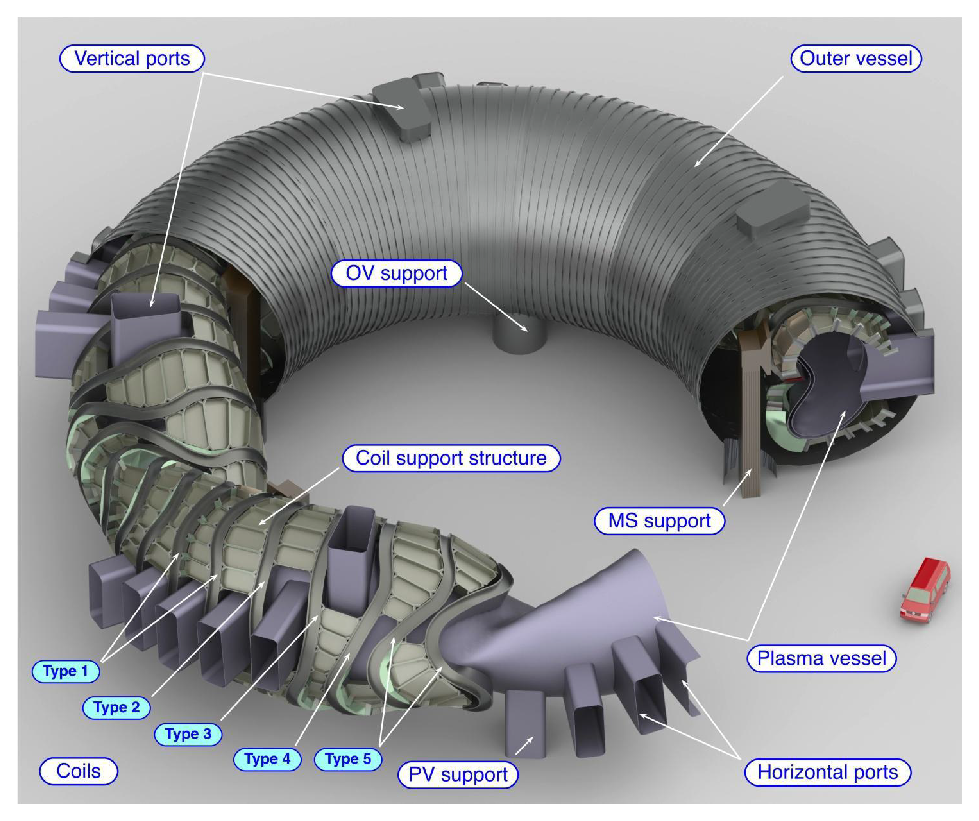
\epsfig{file=helias5b.eps,width=160mm}}
\caption[HELIAS 5-B Stellarator Power Plant Design]
{\label{fig:helias5b}
  \textit{Fusion power core of the HELIAS 5-B conceptual power plant design
    (from~\cite{helias5b})}
}
\end{figure}

\subsection{Stellarator physics}

Much of the physics is identical to that for tokamaks, including the plasma
composition and the fusion power calculations. However, some physics topics do
differ between stellarators and tokamaks, as follows.

\subsubsection{Plasma geometry}

The plasma geometry model uses Fourier coefficients to represent the complex
3-D plasma shape typical of stellarators. A VMEC~\cite{vmec} calculation (or
other equilibrium code that can provide the Fourier coefficients of the LCFS)
must have been performed prior to running with \process. The overall size of
the plasma is scaled correctly for the required (mean) major and minor radii
for the machine being modelled~\cite{geiger}.

It is necessary to provide three input files that define the plasma shape:

\begin{enumerate}

\item Set \texttt{vmec\_info\_file} in the input file to the name of a file
  with the following format (the numbers given are those for the W7-X high
  mirror configuration); in practice only the effective major and minor radius
  values (\texttt{R\_eff} and \texttt{a\_eff}, respectively) and the number of
  field periods are used:

\footnotesize
\begin{verbatim}
R_eff [m]   a_eff [m]   Aspect ratio   Plasma vol [m3]  LCFS surf area [m2]  field periods
5.486576    0.4942638   11.10050       26.45749         133.4281             5.0
\end{verbatim}
\normalsize

\item Set \texttt{vmec\_rmn\_file} in the input file to the name of a VMEC
  output file containing the calculated plasma boundary $R(m,n)$ Fourier
  coefficients, where $m = 0$ to 11 (rows) and $n = -12$ to 12 (columns).

\item Set \texttt{vmec\_zmn\_file} in the input file to the name of a VMEC
  output file containing the calculated plasma boundary $Z(m,n)$ Fourier
  coefficients, where $m = 0$ to 11 (rows) and $n = -12$ to 12 (columns).

\end{enumerate}

This method enables a wide range of potential plasma geometries to be
modelled, if required. The plasma volume, surface area and mean
cross-sectional area are the outputs from the plasma geometry model.

\subsubsection{Absense of plasma current}

Stellarators try to achieve zero plasma current in order to allow safe
divertor operation, so no current scalings are required.

\subsubsection{Beta limit}

The beta limit is assumed to be 5\%, based on 3-D MHD calculations
\cite{Nuhrenberg}. To apply the beta limit, constraint equation no.\ 24 should
be turned on with iteration variable no.\ 36 (\texttt{fbetatry}).

\subsubsection{Density limit}

The density limit relevant to stellarators has been proposed to be~\cite{LHD}
\begin{equation}
n_{\mbox{\scriptsize max}} = 0.25\left( P B_0 / R_0 \, a_p^2\right)^\frac{1}{2}
\end{equation}
where $n$ is the line-averaged electron density in units of
$10^{20}$~m$^{-3}$, $P$ is the absorbed heating power (MW), $B_0$ is the
on-axis field (T), $R_0$ is the major radius (m), and $a_p$ is the plasma
minor radius (m). To enforce the density limit, turn on constraint equation
no.\ 5 with iteration variable no.\ 9 (\texttt{fdene}).

\subsubsection{$\tau_E$ scaling laws}

%- a transport model which employs a predictive confinement time scaling
%derived from 1-D neoclassical and 3-D turbulence simulations

Five confinement time scaling laws relevant to stellarators are present
within \process. The value of switch \texttt{isc} determines which of these is
used in the plasma energy balance calculation.
\begin{eqnarray}
\tau_E\; (\mbox{Large Helical Device~\cite{LHD}: \texttt{isc=21}})
& = & 0.17 \, R_0^{0.75} \, a_p^2 \, \bar{n}_{20}^{0.69} \, B_0^{0.84} \, P^{-0.58} \\
\tau_E\; (\mbox{Gyro-reduced Bohm~\cite{Goldston}: \texttt{isc=22}})
 & = & 0.25 \, B_0^{0.8} \, \bar{n}_{20}^{0.6} \, P^{-0.6} \, a_p^{2.4} \, R_0^{0.6} \\
\tau_E\; (\mbox{Lackner-Gottardi~\cite{LacknerGottardi}: \texttt{isc=23}})
& = & 0.17 \, R_0 \, a_p^2 \, \bar{n}_{20}^{0.6} \, B_0^{0.8} \, P^{-0.6} \, \iota^{0.4} \\
\tau_E\; (\mbox{ISS95~\cite{Stroth}: \texttt{isc=37}})
& = & 0.079 \, R_0^{0.65} \, a_p^{2.21} \, \bar{n}_{19}^{0.51} \, B_0^{0.83}
\, P^{-0.59} \, \bar{\iota}^{0.4} \\
\tau_E\; (\mbox{ISS04~\cite{Yamada}: \texttt{isc=38}})
& = & 0.134 \, R_0^{0.64} \, a_p^{2.28} \, \bar{n}_{19}^{0.54} \, B_0^{0.84}
\, P^{-0.61} \, \bar{\iota}^{0.41}
\end{eqnarray}
Here, $\bar{\iota}$ is the rotational transform, which is equivalent to the reciprocal
of the tokamak safety factor $q$.

\subsubsection{Heating power options}

Stellarators require no current drive, although provision for auxiliary
heating does need to be present. The method by which auxiliary heating power
is supplied is determined by the switch \texttt{isthtr}:
\begin{description}
\item [\texttt{isthtr = 1} :] electron cyclotron resonance heating
\item [\texttt{isthtr = 2} :] lower hybrid heating
\item [\texttt{isthtr = 3} :] neutral beam injection
\end{description}
The value of variable \texttt{pheat} determines the actual amount of auxiliary
heating power (in Watts) to be applied to the plasma. This variable may be
used as an iteration variable (no.\ 11). Switch \texttt{ignite} may be used if
necessary --- see Section~\ref{sec:ignited}.

\subsubsection{Divertor}

Although the divertor has the same function in both stellarators and tokamaks,
the envisaged concepts differ quite substantially. This is not only related to
the different geometry and symmetries but also specifically to the magnetic
configuration. While the inherent axisymmetry of a tokamak allows for
poloidally-continuous single or double divertor configurations, the
periodicity of helical advanced stellarators leads to multiple X-points with a
corresponding chain of magnetic islands. This island structure may be
exploited by carefully placing divertor plates along the stochastic field
lines, naturally leading to a discontinuous divertor, with the individual
plates being placed in a complex 3-D geometry; see Figure~\ref{fig:stelldiv}.

\begin{figure}[tbph]
\centerline{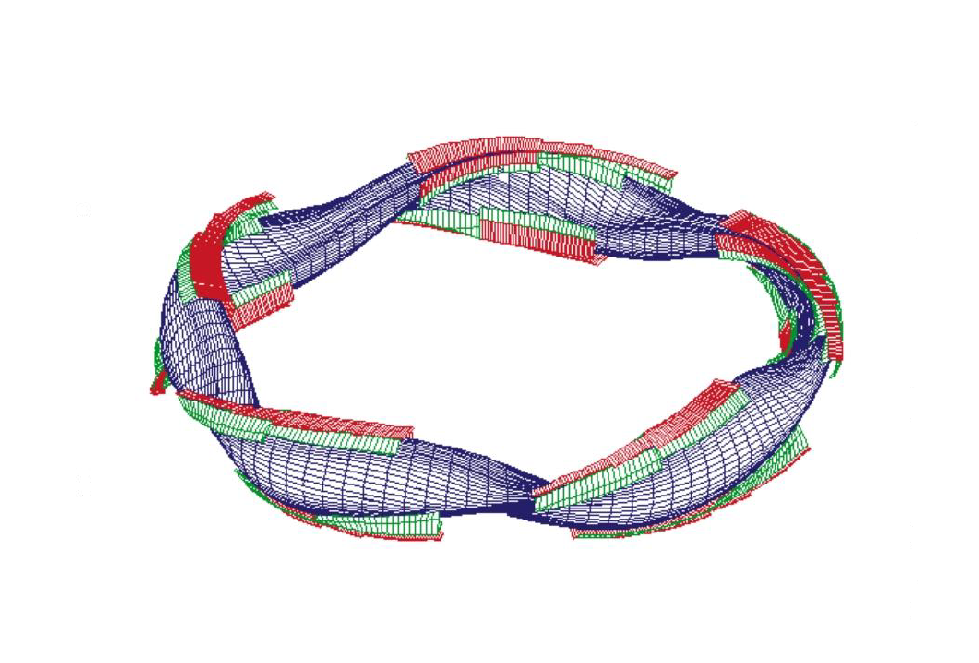
\epsfig{file=stelldiv.eps,width=160mm}}
\caption[Stellarator island divertor configuration]
{\label{fig:stelldiv}
  \textit{A five-period HELIAS plasma (specifically W7-X) with island divertor
    plates shown in red}
}
\end{figure}

Rather than trying to describe the complex physics with a two-point scrape-off
layer model as is used for tokamaks, the stellarator divertor
model~\cite{stell_divertor} is based on fundamental principles which relate
the power crossing the separatrix with an effective wetted area on the
divertor plates allowing the code to estimate the heat load delivered to the
divertor. A basic island divertor model is used which assumes diffusive
cross-field transport and high radiation at the X-point,

The radiated power fraction in the scrape-off layer is given by the input
parameter \texttt{f\_rad}. This is in contrast to the method used for
tokamaks, in which the radiated power fraction is a calculated quantity.

A number of other input parameters may be used to modify the divertor model;
see the variable descriptor file for more details.

\subsection{Machine configuration}

There are a large number of possible stellarator configurations. As stated
earlier, the one chosen for the \process\ model is based on the
\textbf{HELI}cal \textbf{A}dvanced \textbf{S}tellarator (HELIAS) concept, in
which all the coils resemble distorted, non-planar TF coils --- no helical
coils or tokamak-like PF coils are present.  The coil geometry is scaled from
the HELIAS 5-B power plant design, which is based on a five field-period
HELIAS configuration.

\subsubsection{Machine build}
\label{sec:stbuild}

Since a stellarator is inherently non-axisymmetric, the build of the \process\
stellarator is defined in terms of the mean thicknesses of components.

The surface areas for the first wall, blanket and shield components are scaled
linearly with their effective minor radius from the plasma surface area
calculation (the area of a simple torus of circular cross-section is $4 \pi^2
R a$, hence the linear scaling with $a$). The input parameter \texttt{fhole}
may be used to specify the hole fraction, to adjust the surface area to
take account of ports and divertors, for instance. The volumes of the first
wall etc.\ are simply given by the product of their surface area and their
mean thickness.

In contrast to tokamaks, which in \process\ are assumed to have a cylindrical
external cryostat completely surrounding the fusion power core, the
stellarator model assumes that the external cryostat (labelled as the outer
vessel in Figure~\ref{fig:helias5b}) is toroidal with a circular
cross-section. Its cross-section is assumed to be centred at the mean plasma
major radius.

All items external to the fusion power core (buildings, turbines, power
conversion systems, etc.) remain unchanged.

\subsubsection{Stellarator coils}

The stellarator coil model~\cite{stell_coil, stell_coil2} combines scaling
aspects based on the HELIAS 5-B design in combination with analytic inductance
and field calculations.

The fully three-dimensional shape of the coils is assumed to be fixed, but the
sizes of the coils are scaled from the HELIAS 5-B values to the geometrical
values for the machine being modelled using fundamental physics and
engineering principles.

The stellarator coils are assumed to be superconducting --- no resistive coil
calculations are performed.  The critical field at the superconductor is
calculated using circular approximations for the coils in the inductance and
field calculations, and the limit is enforced automatically. Available
superconductors are Nb$_3$Sn (\texttt{isumattf = 1}) and NbTi
(\texttt{isumattf = 3}).

The winding pack cross-section is rectangular for the stellarator coils,
rather than the complicated two-step cross-section assumed for tokamaks. The
coil thicknesses and most of the dimensions of the materials within the coil
cross-section are outputs from the model, instead of being inputs as is the
case for tokamaks; see the variable descriptor file for details. In addition,
certain iteration variables (\texttt{tfcth}, no.\ 13; \texttt{thkcas}, no.\
57; \texttt{cpttf}, no.\ 60 and \texttt{tftort}, no.\ 77) should not be turned
on in the input file as they are calculated self-consistently; the code will
stop with an error message if this is attempted.

\section{Reversed Field Pinch Model}

In addition to the tokamak and stellarator magnetic confinement devices, the
code has the ability to perform calculations based on the physics and
engineering of a reversed field pinch (RFP) device. This third type of
toroidal magnetic device is superficially similar in design to a tokamak (so
therefore shares many of the same components), but the magnetic field
configuration differs.

The model used in \process\ is largely based on the TITAN fusion power
plant~\cite{titan1,titan2}. The following sections summarise its main
features, where they differ from those for tokamaks.

To activate the RFP coding, it is necessary to create a file
\texttt{device.dat}, containing the single character \texttt{2} in the first
row, in the working directory (see Section~\ref{sec:infile}). This has the
effect of setting the internally-used switch \texttt{irfp = 1}. If the file is
absent, or its first character is set to something other than \texttt{2}, the
RFP model is not used, and \texttt{irfp} is set to \texttt{0}.

\subsection{RFP physics}

The plasma in RFPs is circular in cross-section and is axisymmetric.

\subsubsection{Beta limit}

The poloidal beta is limited to a maximum value given by input parameter
\texttt{betpmx} (default = 0.19) using constraint equation~48 and iteration
variable~79 (\texttt{fbetap}).

\subsubsection{Density limit}

No density limit is explicitly coded for RFPs, other than by simply
constraining the upper bound of the electron density variable \texttt{dene}
(iteration variable 6).

\subsubsection{$\tau_E$ scaling law}

One confinement time scaling law relevant to RFPs is present within
\process. The value of switch \texttt{isc} determines the scaling to be used
in the plasma energy balance calculation.
\[
\tau_E\; (\mbox{TITAN RFP~\cite{titan1}: \texttt{isc=25}})
 = 0.05 \, a^2 \, I_p(\mathrm{MA})
\]

\subsubsection{$F$-$\Theta$ plot}

Much of the RFP physics is derived from the characteristic $F$-$\Theta$ plot,
where $F = B_\phi (a)/\langle B_\phi \rangle$, $\Theta = B_\theta (a)/\langle
B_\phi \rangle$, and $\langle B_\phi \rangle$ is the average value of the
toroidal field over the plasma cross-section. Given a value of the pinch
parameter $\Theta$, the corresponding value of the reversal parameter $F$ may
be read from the $F$-$\Theta$ plot, and from these the plasma current and the
current in the TF coils may be obtained using

\begin{eqnarray*}
  B_\theta (a) & = & \frac{\mu_0 I_p}{2\pi a} \\
  B_\phi (a)   & = & \frac{\mu_0 I_{TFC}}{2\pi R}
\end{eqnarray*}
(the second of these assumes that $B_\phi (a)$ is approximately equal to the
vacuum toroidal field at the plasma centre).

The pinch parameter $\Theta$ is set using iteration variable no.\ 78:
\texttt{rfpth}. The corresponding value of the reversal parameter $F$
(\texttt{rfpf}) is calculated using routine \texttt{FTHETA}. $F$ is
constrained to be negative using constraint equation no.\ 49 with f-value
\texttt{frfpf} (iteration variable no.\ 80).

\subsubsection{Current drive}
\label{sec:rfpcd}

The RFP oscillating field current drive option is turned on by setting
\texttt{iefrf = 9}, with a fixed efficiency of 0.8~Amps per Watt of power
injected into the plasma (the coding for this model is, therefore,
trivial). The wall plug to injector efficiency is set using input parameter
\texttt{etaof}, which has a default value of 0.5, and the unit cost is set
using input parameter \texttt{ucof}. The default value for \texttt{ucof} is
3.3~\$ per Watt of injected power.

The bootstrap fraction is assumed to be zero.

Plasma ignition, and additional plasma heating using auxiliary power, are
treated as for tokamaks.

\subsection{TF coils}

The TF coils for the RFP option are derived from the TITAN-II coil set, which
uses circular copper coils. The radial thickness is set using \texttt{tfcth}
as usual, but the toroidal thickness may also be set, using iteration variable
no.\ 77 (\texttt{tftort}). This is constrained to be no larger than is
geometrically possible using constraint equation no.\ 47 with iteration
variable no.\ 76 (\texttt{frfptf}).

\subsection{Ohmic heating coils}

The TITAN-I ohmic heating coil locations, currents etc.\ are assumed. These
comprise 14 copper coils, with currents swinging from positive to negative
during the plasma start-up period, and then decaying back to zero. To account
for different plasma geometries and currents, the ohmic heating coil locations
relative to the plasma centre scale with the TF coil radius and with the
plasma major radius, and the current per turn scales linearly with the plasma
current.

\subsection{EF coils}

The Equilibrium Field coils are based on the TITAN-I EF coils, which are two
superconducting (NbTi) coils that provide the correct vertical field at the
plasma centre. The coil locations scale with the plasma major radius and TF
coil radius along with the ohmic heating coils.

\subsection{Divertor}

The TITAN divertor concept uses three poloidal divertors, which bear little
resemblance to the typical tokamak toroidal divertor systems. The code uses
the TITAN divertor lifetime of one year to enable the divertor costs to be
reasonable, although the divertor surface area (and therefore the cost per
divertor) is likely to be inaccurate.
%!%!%! perhaps we could recalculate divsur properly for RFPs...

\subsection{Code modifications}

As with the stellarator model, the RFP model has been incorporated in such a
way as to allow its simple removal again if required in the future. All new
routines are confined to the dedicated source file \texttt{rfp.f90}. The
tokamak-relevant consistency equations in \process\ (see
Section~\ref{sec:constraints}) are used without modification, to ensure that
the coil currents and the fields they produce are consistent with the plasma
parameters.

\section{Inertial Fusion Energy Model}
\label{sec:ife}

As well as magnetic confinement devices, \process\ has the ability to model
inertial fusion plants, in which a laser or ion beam is used to ignite a
target pellet containing the fusion fuel.

To activate the inertial fusion energy (IFE) coding, it is necessary to create
a file \texttt{device.dat}, containing the single character \texttt{3} in the
first row, in the working directory (see Section~\ref{sec:infile}). This has
the effect of setting the internally-used switch \texttt{ife = 1}. If the file
is absent, or its first character is set to something other than \texttt{3},
the IFE model is not used, and \texttt{ife} is set to \texttt{0}.

The IFE model~\cite{process_ife} is controlled using two additional switches.
\begin{description}
\item [\texttt{ifetyp = 0} :] Generic device build
\item [\texttt{ifetyp = 1} :] OSIRIS-type device build~\cite{osiris1,osiris2,osiris3}
\item [\texttt{ifetyp = 2} :] SOMBRERO-type device build~\cite{sombrero1,sombrero2}
\item [\texttt{ifetyp = 3} :] HYLIFE-II-type device build~\cite{hylife1,hylife2,hylife3}
\end{description}
Switch \texttt{ifetyp} defines the type of device that is assumed; this varies
widely between different conceptual designs. The generic type assumes a
cylindrically symmetric device, while the other types are approximations to
the builds of the given conceptual machines~\cite{ife_build}. In general, the
build from the centre of the device (at the target ignition location) is in
the order: chamber, first wall, gap, blanket, gap, shield, gap, building
wall. The user specifies the thicknesses of these regions, and also the
materials that are present and in what proportions. \Red{[expand]} %!%!%!

\begin{description}
\item [\texttt{ifedrv = -1} :] Driver efficiency and target gain are input as
  functions of driver energy
\item [\texttt{ifedrv = 0} :] Driver efficiency and target gain are input
\item [\texttt{ifedrv = 1} :] SOMBRERO laser drive efficiency and target gain assumed
\item [\texttt{ifedrv = 2} :] OSIRIS heavy ion beam driver efficiency and
  target gain are assumed~\cite{ife_driver}
\end{description}
Switch \texttt{ifedrv} defines how the code calculates the driver efficiency
and target gain --- these are the primary outputs required from the physics
part of the model. For the SOMBRERO and OSIRIS cases (\texttt{ifedrv = 1} and
\texttt{ifedrv = 2}, respectively) the driver efficiency and gain are
calculated from curves of these parameters as functions of the driver
energy. For the \texttt{ifedrv = -1} case, the user provides the driver
efficiency and target gain versus driver energy, via the two arrays
\texttt{etave(1:10)} and \texttt{gainve(1:10)} respectively; the element number
corresponds to the driver energy in MJ, and outside the range 1--10~MJ the
curves are extrapolated linearly. Finally, for the \texttt{ifedrv = 0} case,
the user inputs single values for the driver efficiency (\texttt{drveff}) and
target gain (\texttt{tgain}).

Constraint equation no.\ 50 can be turned on to enable the ignition repetition
rate to remain below a user-specified upper limit (\texttt{rrmax}); iteration
variable no.\ 86 (\texttt{frrmax}) is the associated f-value (see
Section~\ref{sec:constraints}). The other iteration variables relevant for the
IFE model are nos.~81--85 (\texttt{edrive}, \texttt{drveff}, \texttt{tgain},
\texttt{chrad} and \texttt{pdrive} --- see Table~\ref{tab:itvars2}).

\section{Safety and Environment Models}

At present, the neutronics, activation and inventory calculations comprise the
safety and environment models in the code.

The models comprising the safety and environmental calculations~\cite{FISPACT}
within the code are all called from routine \texttt{FISPAC}. They are only
performed once, at the end of each run, as they take a relatively long time to
evaluate, and the results are only used for diagnostic purposes --- no
constraints are imposed at present to minimise doses, for instance.
% AND LOCA in safety.f90...

N.B.\ These models are currently not available in the present version of the
code.

\subsection{Neutronics}

The neutronics module predicts the neutron flux spectra in the inboard and
outboard first wall and blanket components. The spectra are based on a
simplified tokamak device that has a fixed ratio ($=1.5825$) between the
outboard blanket thickness and the inboard blanket thickness, and are scaled
according to the actual thickness of the outboard blanket. This relatively
limited, single-parameter approach is expected to be replaced by a more
general method, which should allow a more accurate portrayal of the device
being modelled by \process.

\subsection{Activation and inventory information}

The code evaluates the consequences of exposing the power plant's materials to
the calculated neutron fluxes, subject to the limitations imposed by the
neutronics module. A library of neutron cross-sections and decay data is used
to calculate the total activity, gamma-ray dose rate and decay heat output due
to the materials' exposure to neutrons, both at the end of the plant's life
and at a time 100 years later. These values are relevant to decommissioning
and disposal studies, and additional parameters that can be obtained from the
nuclide inventory will also be included as the need arises.

\section{Cost Models}

The cost accounting used by \process\ combines methods~\cite{cost1} used in
the TETRA code~\cite{tetra} and the Generomak~\cite{generomak} scheme.  The
costs are split into the standard accounting categories~\cite{cost2} generally
used in the reporting of power plant costs. The best references for the
algorithms used are~\cite{storac}, and source file \texttt{costs.f90} in the
code itself.

The majority of the costed items have a unit cost associated with them. These
values scale with (for example) power output, volume, component mass etc., and
many are available to be changed via the input file. All costs and their
algorithms correspond to 1990 dollars.

\subsection{Cost options}

\subsubsection{$N^{th}$ of a kind costs}

The unit costs of the components of the fusion power core are relevant to
``first-of-a-kind'' items. That is to say, the items are assumed to be
relatively expensive to build as they are effectively prototypes and
specialised tools and machines have perhaps been made specially to create
them. However, if a ``production line'' has been set up, and R \& D progress
has allowed more experience to be gained in constructing the power core
components, the costs will be reduced as a result. Variable \texttt{fkind} may
be used to multiply the raw unit costs of the fusion power core items (by a
factor less than one) to simulate this cost reduction for an
$N^{th}$-of-a-kind device. In other systems studies of fusion power
plants~\cite{galambos}, values for this multiplier have ranged from 0.5 to
0.8.

\subsubsection{Level of safety assurance}

Many of the unit costs have four possible choices, relating to the level of
safety assurance~\cite{lsa} flag \texttt{lsa}. A value \texttt{lsa = 1}
corresponds to a plant with a full safety credit (i.e.\ is truly passively
safe). Levels \texttt{2} and \texttt{3} lie between the two extremes, and
level \texttt{4} corresponds to a present day fission reactor, with no safety
credit.

\subsubsection{Replaceable components}

The first wall, blanket, divertor, centrepost (if present) and current drive
system have relatively short lifetimes because of their hostile environment,
after which they must be replaced. Because of this frequent renewal they can
be regarded as though they are ``fuel'' items, and can be costed
accordingly. Switch \texttt{ifueltyp} is used to control whether this option
is used in the code. If \texttt{ifueltyp = 1}, the costs of the first wall,
blanket, divertor and a fraction \texttt{fcdfuel} of the cost of the current
drive system are treated as fuel costs. If \texttt{ifueltyp = 0}, these are
treated as capital costs.

\subsubsection{Cost of electricity calculations}

Switch \texttt{ireactor} determines the type of cost of electricity
calculation that is performed. If \texttt{ireactor = 0}, no cost of
electricity calculation is performed. If \texttt{ireactor = 1}, then the cost
of electricity is evaluated, with the value quoted in units of m\$/kWh.

\subsubsection{Net electric power calculation}

Related to the cost of electricity is the net electric power calculation
performed in routine \texttt{POWER}. It is possible that the net electric
power can become negative due to a high recirculating power. Switch
\texttt{ipnet} determines whether the net electric power is scaled to always
remain positive (\texttt{ipnet = 0}), or whether it is allowed to become
negative (\texttt{ipnet = 1}), in which case no cost of electricity
calculation is performed.

\section{Other Switches and Models}

\subsection{Diagnostic output}

Switch \texttt{verbose} can be set to \texttt{1} in the input file to allow
the code to write some additional diagnostic output to the screen. Currently,
extra information about the progress of the optimiser is produced. This
setting is likely to be of interest only to ``expert'' users.

\subsection{Code parameters affecting other models}

This chapter has summarised the methods by which several of the models in the
code can be activated. There are many others present, however, and it is
suggested that the user refers to the variable descriptor file,
\texttt{vardes.html}. As stated earlier in Section~\ref{sec:vardes}, this
contains details of all the parameters within the code that can be changed by
the user, in order to customise the machine modelled by \process.

  %  Physics, Engineering and Other Models
\mychapter{Running \process}
\label{chap:run}

The intention of this chapter is to provide a comprehensive prescription for
setting up and performing runs with the code.  Firstly, the input file's
structure and format is described. The user is then taken through the
procedure for setting up the code to model a new machine, and finally an
attempt is made to indicate and solve the problems that the user will face
whilst trying to achieve a feasible solution.

\section{Environment set-up}
\label{sec:run_environment}

 \process\ is available for execution from the CCFE Fusion Unix Network, on which you must have an account.

To set up your environment to be able to run the code, the user interface and the associated
utilities (see Chapter~\ref{chap:utilities}), add the following lines to your \texttt{.bashrc} file.  This is a file in the user's home directory, assuming the bash Unix shell is being used.  Although hidden, it can be opened by issuing the relevant command, for example \texttt{gedit .bashrc}.
\begin{quote}
\begin{verbatim}
module use /home/PROCESS/modules
module swap python
module load process/master
\end{verbatim}
\end{quote}
(If you want to use the latest draft version of the code instead of the latest verified release version, replace \texttt{module load process/master} with \texttt{module load process/develop} above.)

\section{User Interface}
\label{sec:gui}
The user interface allows for viewing and editing of \indat\ files in a web browser. Launch the interface (GUI) by typing \verb+start_gui+ from the Unix command line. 

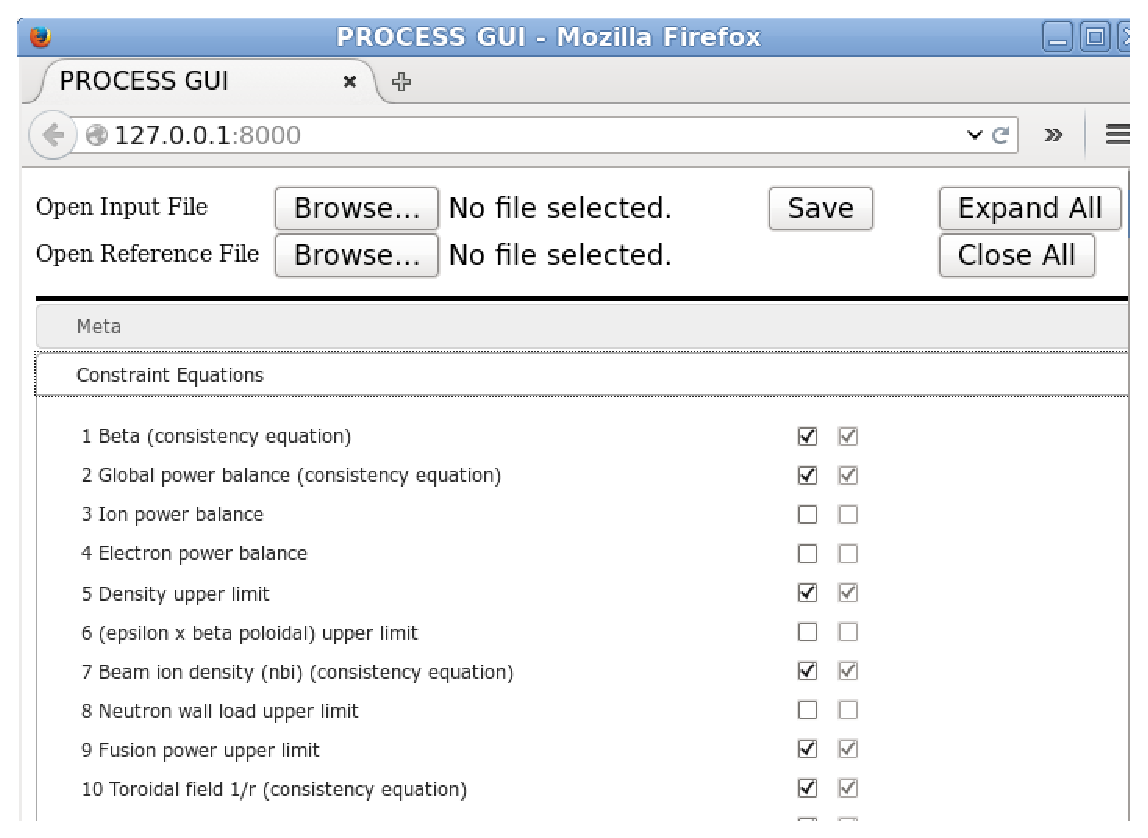
\includegraphics[scale=1]{gui.eps}

Every variable is listed along with its current value, a 'reference'
value and a short description. Hovering over the short description will
provide a longer description. Until an input file is opened, all values are given their default values assigned by \process. 

The reference values are used to compare differences between two files.
Differences between the reference value and the current input value will be
highlighted in red.

The 'Meta' section allows editing of the run description, which will be placed at the top of the created \indat. Iteration variables and constraint equations can be enabled using the checkboxes in the relevant sections.

An input file and a reference file can be opened using the buttons at the top
of the window. The files opened must be compatible with the \process\ version
number shown in the top right of the window.

The 'Save' button creates an \indat\ file with a similar layout to the GUI. Variables whose values are set different from the \process\ default are listed under module headings, along with a comment describing the variable. For integer variables, a description of the value
selected may also be included. The variables \texttt{neqns} (number of constraints) and \texttt{nvar} (number of iteration variables) are automatically calculated.

When using the Firefox web browser it can save time to select \\
\texttt{Preferences > General > Downloads > Always ask me where to save files.}

You can searching for a particular variable can be done using the browser's in-built search. Use the "Expand" button in the top-right of the window to expand every module heading and use Ctrl-f to search.

\section{Executing the Code}

Execute \process\ by simply typing \texttt{process} on the Unix command line.

By default, the input and output file names are as described in the following
sections. If, however, \process\ is executed with an argument, this is used as
a prefix to the file names:
\begin{quote}
\begin{verbatim}
process myrun
\end{verbatim}
\end{quote}
will assume that the input file is called \textit{myrun}\indat, etc.

The input file must be in the current directory.  The output files \textit{myrun}\outdat\
and \textit{myrun}\mfile\ will be created in the current directory.

\section{The Input File}
\label{sec:infile}

The input file \indat\ is used to change the values of the physics,
engineering and other code parameters from their default values, and to set up
the numerics (constraint equations, iteration variables etc.) required to
define the problem to be solved.  The user interface writes the input file, so
it is not necessary to edit it directly.  Details of layout and format are in
Appendix~\ref{app:infile}.

If the code encounters a problem reading the input file, it will stop
immediately with an error message. The last line of the output file \outdat\
may give an indication of where in the input file the problem lies.

\section{The Output Files}

The main output from the code is sent to file \outdat\ in the working
directory.  It is essential to check that the code reports that it has found a
\textit{feasible solution}.

A second file, \mfile, is also produced in the working directory.  This file
contains most of the same data as \outdat\ but in a different format, and has
been designed to be ``machine-readable'' by some of the utility programs
described in Chapter~\ref{chap:utilities}, to allow simple post-processing and
graphical output to be produced easily.

\section{Optimisation mode}

Switch \texttt{ioptimz} should be set to \texttt{1} for optimisation mode. 

If \texttt{ioptimz = 0}, a non-optimisation pass is performed first.  Occasionally this provides a feasible set of initial conditions that aids convergence of the optimiser, but it is recommended to use \texttt{ioptimz = 1}. 

Enable all the relevant consistency equations, and it is advisable to enable the corresponding iteration variables shown in bold in Table~\ref{tab:eqns}. A number of limit equations (inequality constraints) can also be activated.  For limit equations, the corresponding f-value must be selected as an iteration variable.  In optimisation mode, the number of iteration variables is unlimited.

It may still be difficult, if not impossible, to reconcile the fusion power
and the net electric power with the required values. This may well be due to
the power conversion efficiency values being used --- refer to
Figure~\ref{fig:powerflow3}.

With luck, a few iterations of this process will produce an adequate benchmark
case. A typical input file for use with \process\ in non-optimisation mode is
contained in Appendix~\ref{app:infile1}.

If scans of a given variable are to be made over a large range of
values, it is often a good idea to start the scan in the middle of the desired
range, and to split the scan in two --- one going downwards from the initial
value, and the other upwards.  This ensures that the whole range of the scan
produces well-converged machines (assuming a ``good'' initial point), without
sharp changes in gradient in the parameter values.

It should be remembered that the value of the scan variable is set in the
array \texttt{sweep}, and this overrules any value set for the variable
elsewhere in the input file. 

The output from an optimisation run contains an indication as to which iteration variables lie at their limiting values. A typical input file for use with \process\ in optimisation mode is contained in Appendix~\ref{app:infile2}.

\section{Non-optimisation mode}
\label{sec:optim}

Non-optimisation mode is sometimes used to perform benchmark comparisons, whereby the
machine size, output power etc.\ are known and one only wishes to find the
calculated stresses, beta values and fusion powers, for example. 

Running \process\ in non-optimisation mode requires few changes to be made to the
input file from the non-optimisation case. The main differences between
optimisation mode and non-optimisation mode are:

\begin{enumerate}

\item Non-optimisation mode does NOT apply lower or upper bounds to the iteration
  variables.  It follows that limit equations are not enforced.

\item In non-optimisation mode the number of active iteration variables must be equal to the number of constraints.

\item A figure of merit is not available in non-optimisation mode.

\item Scans cannot be performed in non-optimisation mode.

\end{enumerate}

As before, the user must decide which constraint equations and iteration
variables to activate. 


\section{Troubleshooting}
\label{sec:problems}

Experience has shown that the first few attempts at running \process\ with a
new input file tends to produce unfeasible results --- that is, the code will
not find a consistent set of machine parameters. The highly non-linear nature
of the numerics of \process\ is the reason for this difficulty, and it often
requires a great deal of painstaking adjustment of the input file to overcome.  The utility 
\texttt{a\_to\_b} (~\autoref{sec:atob}) is useful in this situation.

\subsection{Error handling}
\label{sec:errors}

In general, errors detected during a run are handled in a consistent manner,
with the code producing (hopefully) useful diagnostic messages to help the
user understand what has happened.

There are three levels of errors and warning that may occur:
\begin{description}

\item{Level 1:} An \textit{informational}\/ message is produced under certain
  conditions, for example if the code has modified the user's input choice for
  some reason.

\item{Level 2:} A \textit{warning}\/ message is produced if a non-fatal situation has
  occurred that may result in an output case that is inaccurate or
  unreliable in some way.

\item{Level 3:} An \textit{error}\/ message will occur if a severe or fatal
  error has occurred and the program cannot continue.

\end{description}

These messages are printed on the screen during the course of a run, and those
still active at the final (feasible or unfeasible) solution point are also
written to the end of the output file (messages encountered during the
iteration process are not copied to the output file, as the convergence to a
valid solution might resolve some of the warnings produced earlier in the
solution process).

The \texttt{error\_status} variable returns the highest severity level that
has been encountered (or zero if no abnormal conditions have been found); if a
severe error (level 3) is flagged at any point the program is terminated
immediately. The final message number encountered during a run is returned via
output variable \texttt{error\_id}. In addition, with certain messages, a
number of diagnostic values may also be given; these can be used to provide
extra diagnostic information if the source code is available.

\subsection{General problems}

A code of the size and complexity of \process\ contains myriads of equations
and variables. Virtually everything depends indirectly on everything else
because of the nature of the code structure, so perhaps it is not surprising
that it is often difficult to achieve a successful outcome.

Naturally, problems will occur if some of the parameters become unphysical.
For example, if the aspect ratio becomes less than or equal to one, then we
must expect problems to appear. For this reason, the bounds on the
iteration variables should be selected with care.

Occasionally arithmetic (``\texttt{NaN}'') errors are reported. They usually occur when the code is exploring unphysical values of the parameters, and often suggest that no feasible solution exists for the input file used.

The error messages produced by the code attempt to provide diagnostic
information, telling the user where the problem occurs, and also suggest a
possible solution. These messages are out of necessity brief, and so cannot
promise to lead to a more successful outcome.

There is the option to turn on extra debugging output; to do this, set \texttt{verbose = 1} in the input file.

\subsection{Optimisation problems}

On reflection it is perhaps surprising that \process\ ever does manage to
find the global minimum figure of merit value, since if there are
\texttt{nvar} iteration variables active the search is over
\texttt{nvar}-dimensional parameter space, in which there may be many shallow
minima of approximately equal depth. Remember that \texttt{nvar} is usually of
the order of twenty.

The machine found by \process\ may not, therefore, be the absolutely optimal
device. It is quite easy to have two or more solutions, with results only a
few per cent different, but a long way apart in parameter space. The technique
of ``stationary'' scans is sometimes used in this situation: a scan is requested, but the same value of the scan variable is listed repeatedly.

Scans should be started in the middle of a range of values, to try to keep the
scan within the same family of machines. The optimum machine found may
otherwise suddenly jump to a new region of parameter space, causing the output
variables to seem to vary unpredictably with the scanning variable.

It should be noted that in general the machine produced by \process\ will
always sit against one or more operation limits. If, during a scan, the limit
being leant upon changes (i.e.\ if the machine jumps from leaning on the beta
limit to leaning on the density limit) the output parameters may well become
discontinuous in gradient, and trends may suddenly change direction.

\subsection{Unfeasible results}

In the numerics section of the output file, the code indicates whether the run
produced a feasible or unfeasible result.

The former implies a successful outcome, although it is always worth checking
that the sum of the squares of the constraint residuals (\texttt{sqsumsq}) is small ($\sim
10^{-3}$ or less); the code will issue a warning if the solver reports convergence but
the value of \texttt{sqsumsq} exceeds $10^{-2}$. If this occurs, reducing the
value of the HYBRD tolerance \texttt{ftol} or \vmcon\ tolerance
\texttt{epsvmc} as appropriate should indicate whether the result is valid
or not; the output can usually be trusted if (1) the constraint
residues\footnote{The constraint residues are the final values of $c_i$ in the
  constraint equations --- see Section~\ref{sec:constraints}. The value
  \texttt{sqsumsq} is the square root of the sum of the squares of these
  residuals.} fall as the tolerance is reduced to about $10^{-8}$, and (2) the
code indicates that a feasible solution is still found.

An unfeasible result occurs if \process\ cannot find a set of values for the
iteration variables which satisfies all the given constraints. In this case,
the values of the constraint residues shown in the output give some indication
of which constraint equations are not being satisfied --- those with the
highest residues should be examined further. In optimisation mode, the code
also indicates which iteration variables lie at the edge of their allowed
range.

Unfeasible runs can be caused by specifying physically incompatible input parameters,  using insufficient iteration variables, or by starting the problem with unsuitable values of the iteration variables. 

The utility \texttt{run\_process} (Section~\ref{subsec:run_process}) carries out many runs, changing the starting values of the iteration variables randomly.  It stops once a feasible solution is found.

Another approach is to start with an input file that gives a feasible solution, and modify it step by step towards the parameters desired.  This process is automated by the 
utility \texttt{a\_to\_b} ((Section~\ref{sec:atob}).

It is important to choose the right number of \textit{useful}\/ iteration variables for the
problem to be solved --- it is possible to activate too many iteration variables as well as too few, some of which may be redundant.

Both optimisation and non-optimisation runs can fail with an error message
suggesting that the iteration process is not making good progress. This is
likely to be due to the code finding itself unable to escape a region of the
parameter space where the minimum in the residuals is significantly above
zero. In this situation, there is either no solution possible (the residuals
can therefore never approach zero), or the topology of the local minimum makes
it difficult for the code to escape to the global minimum. Again, a helpful
technique is to either change the list of iteration variables in use, or to
simply modify their initial values to try to help the code avoid such regions.

A technique that occasionally removes problems due to unfeasible results,
particularly if an error code \texttt{ifail = 3} is encountered during an
optimisation run, is to adjust slightly one of the limits imposed on the
iteration variables, even if the limit in question has not been reached. This
subtly alters the gradients computed by the code during the iteration process,
and may tip the balance so that the code decides that the device produced is
feasible after all. For instance, a certain component's temperature might be
400~K, and its maximum allowable temperature is 1000~K\@. Adjusting this limit
to 900~K (which will make no difference to the \textit{actual}\/ temperature)
may be enough to persuade the code that it has found a feasible solution.

Similarly, the order in which the constraint equations and iteration variables
are stored in the \texttt{icc} and \texttt{ixc} arrays can make the difference
between a feasible and unfeasible result. This seemingly illogical behaviour
is, sadly, typical of the way in which the code works.

Another technique in such situations may be to change the finite difference
step length \texttt{epsfcn}, as this might subtly change the path taken in the
approach towards a solution.

It may be the case that the act of satisfying all the required constraints is
impossible. No machine can exist if the allowed operating regime is too
restrictive, or if two constraint equations require conflicting
(non-overlapping) parameter spaces. In this case some relaxation of the
requirements is needed for the code to produce a successful machine design.

\subsection{Hints}

The above sections should indicate that it is the complex interplay between
the constraint equations and the iteration variables that determines whether
the code will be successful at producing a useful result. It can be a somewhat
laborious process to arrive at a working case, and (unfortunately, perhaps)
experience is often of great value in this situation.

It should be remembered that sufficient iteration variables should be used to
solve each constraint equation. For instance, a particular limit equation may
be $A \leq B$, i.e.\ $A = fB$, where the f-value $f$ must lie between zero and
one for the relation to be satisfied.  However, if none of the iteration
variables have any effect on the values of $A$ and $B$, and $A$ happens to be
\textit{greater}\/ than $B$, then \process\ will clearly not be able to solve
the constraint.

The lower and upper bounds of the iteration variables are all available to be
changed in the input file. Constraints can be relaxed in a controlled manner
by moving these bounds, although in some cases care should be taken to ensure
that unphysical values cannot occur.  The code indicates which iteration
variables lie at the edge of their range.

It is suggested that constraint equations should be added one at a time, with
sufficient new iteration variables activated at each step.  If the situation
becomes unfeasible it can be helpful to reset the initial iteration variable
values to those shown in the output from a previous feasible case, and rerun
the code.

  %  Execution of the Code
\mychapter{Changing the Source Code: New Models, Variables and Constraints}
\label{chap:modify}

It is often useful to add extra features to the code in order to model new
situations. This chapter provides instructions on how to do this, with
specific details on how to add various numerics related items to \process.

Please remember to modify the relevant sections and table(s) in this User
Guide if changes are made to the source code!

\section{Source Code Modification}
\label{sec:codemods}

Described here are the general rules that apply when the Fortran source code
is modified. See Section~\ref{sec:code_release} for instructions on how to
commit changes to the \process\ Git repository and produce new releases. The variable descriptor file is generated from specially-formatted comment lines within the source code (see Section~\ref{sec:autodoc} for more details). Therefore, it is exceedingly important to keep these lines relevant and in sync with the variables they describe.

\subsection{Changing the Fortran code}

Please ensure that the following rules are adhered to when modifying the
\process\ source code:

\begin{enumerate}

\item Keep the layout consistent in with the existing code,
  including indentation of clauses (\texttt{if}-statements, \texttt{do}-loops,
  etc.).

\item Use the standard routine header (see below).

\item Always use \verb+implicit none+ and declare all local variables
  explicitly.

\item Declare all `real' (i.e.\ floating-point) variables as
  \texttt{real(kind(1.0D0))}.

\item Ensure all routine arguments have the appropriate attribute \texttt{intent(in)},
  \texttt{intent(out)} or \texttt{intent(inout)}, as necessary.

\item Always write explicit real constants using the scientific \texttt{D}
  notation, e.g.\ \texttt{1.0D0}, \texttt{2.3D0}, \texttt{-1.23D6}. That is to
  say, use \texttt{1.0D0} and not \texttt{1.0} or \texttt{1.} or \texttt{1} when the
  expression should be using floating-point arithmetic.

\end{enumerate}

A Fortran 90/95 manual, complete with guidelines for good Fortran 90/95
practice, may be found at the following webpage:
\begin{center}
\texttt{
\href{http://fusweb1.fusion.ccfe.ac.uk/~pknight/f95notebook.html}
{http://fusweb1.fusion.ccfe.ac.uk/$\sim$pknight/f95notebook.html}
}
\end{center}

\subsection{Source code documentation}

It is critically important to keep the documentation in the source code itself
up-to-date, relevant and tidy. Please keep to the following guidelines
whenever the source code is modified.
\begin{enumerate}

\item Use comments copiously in the code.

\item Use the standard header layout, and do not omit any of the
  sections. Here is an example subprogram header:
\footnotesize
\begin{verbatim}
  ! !!!!!!!!!!!!!!!!!!!!!!!!!!!!!!!!!!!!!!!!!!!!!!!!!!!!!!!!!!!!!!!!!!

  subroutine culblm(bt,dnbeta,plascur,rminor,betalim)

    !+ad_name  culblm
    !+ad_summ  Beta scaling limit
    !+ad_type  Subroutine
    !+ad_auth  P J Knight, CCFE, Culham Science Centre
    !+ad_cont  N/A
    !+ad_args  bt      : input real :  toroidal B-field on plasma axis (T)
    !+ad_args  dnbeta  : input real :  Troyon-like g coefficient
    !+ad_args  plascur : input real :  plasma current (A)
    !+ad_args  rminor  : input real :  plasma minor axis (m)
    !+ad_args  betalim : output real : beta limit as defined below
    !+ad_desc  This subroutine calculates the beta limit, using
    !+ad_desc  the algorithm documented in AEA FUS 172.
    !+ad_desc  <P>The limit applies to beta defined with respect to the total B-field.
    !+ad_desc  Switch ICULBL determines which components of beta to include (see
    !+ad_desc  routine <A HREF="constraints.html">constraints</A> for coding):
    !+ad_desc  <UL>
    !+ad_desc  <P><LI>If ICULBL = 0, then the limit is applied to the total beta
    !+ad_desc  <P><LI>If ICULBL = 1, then the limit is applied to the thermal beta only
    !+ad_desc  <P><LI>If ICULBL = 2, then the limit is applied to the thermal +
    !+ad_desc                        neutral beam beta components
    !+ad_desc  </UL>
    !+ad_desc  The default value for the g coefficient is DNBETA = 3.5
    !+ad_prob  None
    !+ad_call  None
    !+ad_hist  21/06/94 PJK Upgrade to higher standard of coding
    !+ad_hist  09/11/11 PJK Initial F90 version
    !+ad_hist  27/06/13 PJK Modified header comments
    !+ad_stat  Okay
    !+ad_docs  AEA FUS 172: Physics Assessment for the European Reactor Study
    !+ad_docs  AEA FUS 251: A User's Guide to the PROCESS Systems Code
    !
    ! !!!!!!!!!!!!!!!!!!!!!!!!!!!!!!!!!!!!!!!!!!!!!!!
\end{verbatim}
\normalsize
  A description of all the available automatic documentation marker tags
  (these all start with \verb.!+ad_.) may be found by examining the main
  program header of the (self-documenting!) automatic documentation program
  itself (in file \texttt{autodoc.f90}).

\item After \textbf{every}\ change within a routine, add a new history line
  (using \verb.!+ad_hist., and \verb.!+ad_hisc. for continuation lines) to its
  header. Ensure that all routines called are listed via
  \verb.!+ad_call. lines.  Update the description lines as necessary. You may
  use html tags and hyperlinks (some are shown in the example above) as
  required; to be sure that they have been added correctly, type \texttt{make
    html} to create the web documentation and examine the relevant html file
  (i.e.\ \texttt{culblm.html} for the example above) using your favourite web
  browser.

\item If you add a new routine to a module, remember to modify the header of the module as well as that of the new routine (add a \verb.!+ad_cont. line to it).

\item Add suitable documentation to this User Guide whenever a
  model is added or modified. This should be done immediately to ensure that
  the Guide remains consistent with the source code. Change the code's revision
  number and the date in \texttt{process.tex}.
  
\item Add a new file to the folder \texttt{release\_notes}.  It is particularly important to describe here any changes to the required IN.DAT - especially any change that makes previous IN.DAT files unusable.  

\end{enumerate}

\section{Input Parameters}

Input parameters (see Section~\ref{sec:inpars}) are added to the code in the
following way:

\begin{enumerate}

\item Choose the most relevant module (usually one of those in source file
  \texttt{global\_variables.f90}). Keeping everything in alphabetical order
  (or possibly within a group of variables closely-related to a particular
  switch), add a declaration statement for the new variable, specifying a
  ``sensible'' default value, and a correctly formatted comment line to
  describe the variable. Copy the examples already present, such as
\begin{verbatim}
  !+ad_vars  abktflnc /5.0/ : allowable first wall/blanket neutron
  !+ad_varc                   fluence (MW-yr/m2) (blktmodel=0)
  real(kind(1.0D0)) :: abktflnc = 5.0D0
\end{verbatim}
  Note that the automatic documentation marker tag \verb.!+ad_vars. tells the
  \texttt{autodoc} utility (Section~\ref{sec:autodoc}) that the line is (the
  first line of) a variable description, while \verb.!+ad_varc. specifies any
  continuation lines. Also note that the colon (:) on the first line is
  necessary, as it is assumed to exist by the dictionary-building Python
  utility for the GUI\@.

\item Add a dated comment (using \verb.!+ad_hist.) to the header of the
  relevant module.

\item Ensure that all the modules that use the new variable reference the
  relevant module via the Fortran \texttt{use} statement.

\item Add the parameter to routine \texttt{PARSE\_INPUT\_FILE} in source file
  \texttt{input.f90} in a suitable place --- keep to alphabetical order. The
  existing examples provide guidance on how to do this. Note that real (i.e.\
  double precision) and integer variables are treated differently, as are
  scalar quantities and arrays.

%\item Modify \texttt{process\_dicts.py} and \texttt{write\_constraints.conf}
%  accordingly.

\end{enumerate}

\section{Iteration Variables}

New iteration variables (see Section~\ref{sec:itvars}) are added in the
same way as input parameters, with the following additions:

\begin{enumerate}

\item Increment the parameter \texttt{ipnvars} in module \texttt{numerics} in
  source file \texttt{numerics.f90} in order to accommodate the new iteration
  variable.

\item Add an additional line to the initialisation of the array \texttt{ixc}
  in module \texttt{numerics} in source file \texttt{numerics.f90}.

\item Assign sensible values for the variable's bounds to the relevant
  elements in arrays \texttt{boundl} and \texttt{boundu} in module
  \texttt{numerics} in source file \texttt{numerics.f90}.

\item Assign the relevant element of character array \texttt{lablxc} to the
  name of the variable, in module \texttt{numerics} in source file
  \texttt{numerics.f90}.

\item Add the variable to routines \texttt{LOADXC} and \texttt{CONVXC} in
  source file \texttt{iteration\_variables.f90}, mimicking the way that the
  existing iteration variables are coded.

\item Modify the variable's description in its declaring module (which is
  likely to be in source file \texttt{global\_variables.f90}), to say that it
  is ``(iteration variable XXX)''

\item Add dated comments (using \verb.!+ad_hist.) to the headers of
  all affected routines and modules.

\item Modify Table~\ref{tab:itvars3} of this User Guide
  (\texttt{UserGuide\_Chapter2.tex}).

%\item Modify \texttt{process\_dicts.py} and \texttt{write\_constraints.conf}
%  accordingly.

\end{enumerate}

If an existing input parameter is now required to be an iteration variable,
then simply carry out the tasks mentioned here.

It should be noted that iteration variables must not be reset elsewhere in the
code. That is, they may only be assigned new values when originally
initialised (in the relevant module, or in the input file if required), and in
routine \texttt{CONVXC} where the iteration process itself is performed.
Otherwise, the numerical procedure cannot adjust the value as it requires, and
the program will fail.

\section{Other Global Variables}

This type of variable embraces all those present in the modules in
\texttt{global\_variables.f90} (and some others elsewhere) which do not need
to be given initial values or to be input, as they are calculated within the
code. These should be added to the code in the following way:

\begin{enumerate}

\item Choose the most relevant module (usually one of those in source file
  \texttt{global\_variables.f90}). Keeping everything in alphabetical order
  (or possibly within a group of variables closely-related to a particular
  switch), add a declaration statement for the new variable, specifying the
  initial value \texttt{0.0D0}, and a correctly formatted comment line to
  describe the variable (copying the examples already present --- see also
  ``Input Parameters'' above).

\item Ensure that all the modules that use the new variable reference the
  relevant module via the Fortran \texttt{use} statement.

\end{enumerate}

\section{Constraint Equations}

Constraint equations (see Section~\ref{sec:constraints}) are added to
\process\ in the following way:

\begin{enumerate}

\item Increment the parameter \texttt{ipeqns} in module \texttt{numerics} in
  source file \texttt{numerics.f90} in order to accommodate the new constraint.

\item Add an additional line to the initialisation of the array \texttt{icc}
  in module \texttt{numerics} in source file \texttt{numerics.f90}.

\item Assign a description of the new constraint to the relevant element of
  array \texttt{lablcc}, in module \texttt{numerics} in source file
  \texttt{numerics.f90}.

\item Add a new Fortran \texttt{case} statement containing the new constraint
  equation to routine \texttt{CONSTRAINT\_EQNS} in source file
  \texttt{constraint\_equations.f90}, ensuring that all the variables used in
  the formula are contained in the modules specified via \texttt{use}
  statements present at the start of this file.  Use a similar formulation to
  that used for the existing constraint equations, remembering that the code
  will try to force \texttt{cc(i)} to be zero.

\item Add dated comments (using \verb.!+ad_hist.) to the headers of
  all affected routines and modules.

\item Modify Table~\ref{tab:eqns2} of this User Guide
  (\texttt{UserGuide\_Chapter2.tex}).

\end{enumerate}

Remember that if a limit equation is being added, a new f-value iteration
variable may also need to be added to the code.

\section{Figures of Merit}

New figures of merit (see Section~\ref{sec:foms}) are added to \process\ in
the following way:

\begin{enumerate}

\item Increment the parameter \texttt{ipnfoms} in module \texttt{numerics} in
  source file \texttt{numerics.f90} to accommodate the new figure of merit.

\item Assign a description of the new figure of merit to the relevant element
  of array \texttt{lablmm} in module \texttt{numerics} in source file
  \texttt{numerics.f90}.

\item Add the new figure of merit equation to routine \texttt{FUNFOM} in
  source file \texttt{evaluators.f90}, following the method used in the
  existing examples. The value of \texttt{fc} should be of order unity, so
  select a reasonable scaling factor if necessary. Ensure that all the
  variables used in the new equation are contained in the modules specified
  via \texttt{use} statements present at the start of this file.

\item Add dated comments (using \verb.!+ad_hist.) to the headers of
  all affected routines and modules.

\item Modify Table~\ref{tab:foms} of this User Guide
  (\texttt{UserGuide\_Chapter2.tex}).

%\item Modify \texttt{process\_dicts.py} accordingly.

\end{enumerate}

\section{Scanning Variables}

Scanning variables (see Section~\ref{sec:scans}) are added to \process\ in
the following way:

\begin{enumerate}

\item Increment the parameter \texttt{ipnscnv} in module \texttt{scan\_module}
  in source file \texttt{scan.f90} to accommodate the new scanning variable.

\item Add a short description of the new scanning variable to the
  \texttt{nsweep} entry in source file \texttt{scan.f90}.

\item Add a new assignment to the relevant part of routine \texttt{SCAN} in
  source file \texttt{scan.f90}, following the examples already present,
  including the inclusion of a short description of the new scanning variable
  in variable \texttt{xlabel}.

\item Ensure that the scanning variable used in the assignment is contained in
  one of the modules specified via \texttt{use} statements present at the
  start of this routine.

\item Add dated comments (using \verb.!+ad_hist.) to the headers of
  all affected routines and modules.

\item Modify Table~\ref{tab:scans} of this User Guide
  (\texttt{UserGuide\_Chapter2.tex}).

%\item Modify \texttt{process\_dicts.py} if necessary.

\end{enumerate}

\section{Submission of New Models}

The \process\ source code is maintained by CCFE, and resides in a
\textit{Git}~\cite{git} repository on the CCFE servers. We welcome
contributions of alternative or improved models and algorithms.

We request that contributors provide the following information for any new models that they provide:

\begin{itemize}

\item A comprehensive description of the model; please provide a full list of
  references.

\item A list of all inputs and outputs: descriptions, default (input) values,
  allowed ranges, units.

\item If possible, please cross-reference any input/output variables to
  existing global variables listed in the variable descriptor file (see
  Section~\ref{sec:vardes}).

\item Any new input parameters, iteration variables, constraint equations, figures of merit etc.

\item A definition of any pre-requisites.

\item Any available test data, code examples or test programs in any language.

\end{itemize}

\section{Code Structure}

\subsection{Numerics modules}
\label{sec:numerics_modules}

These modules contain the equation solvers, their calling routines and other
relevant procedures. Various mathematical routines from a number of standard
libraries are also incorporated into these files. Table~\ref{tab:numerics}
summarises the numerics source files.

% Table summarising numerics modules in PROCESS
\begin{table}[tbph]
\footnotesize
\begin{center}
\begin{tabular}{||l||l||} \hline
source file   & description \\ \hline
\texttt{caller.f90} & calls physics, engineering, building and cost routines \\
\texttt{constraint\_equations.f90} & defines the constraint equations \\
\texttt{evaluators.f90} & function evaluators for HYBRD and \vmcon\ packages \\
\texttt{iteration\_variables.f90} & adjusts values of iteration variables \\
\texttt{maths\_library.f90} & miscellaneous `black-box' maths routines,
including HYBRD and \vmcon \\
\texttt{numerics.f90} & numerics array definitions, and calling routines for
HYBRD and \vmcon\ packages \\
\texttt{scan.f90} & performs a parameter scan \\
\hline
\end{tabular}
\end{center}
\caption[Summary of numerics modules]
{\label{tab:numerics}
  \textit{Summary of the numerics modules in \process.}
}
\end{table}

\subsection{Physics modules}

These modules contain the main physics routines that evaluate the plasma and
fusion parameters. Also included here are the routines describing the current
drive and divertor systems. Table~\ref{tab:physics} summarises the main physics
source files.

% Table summarising physics modules in PROCESS
\begin{table}[tbph]
\begin{center}

\begin{tabular}{||l||l||} \hline
source file   & description \\ \hline
\texttt{current\_drive.f90} & current drive efficiency calculations \\
\texttt{divertor.f90} & divertor model calculations\\
\texttt{fispact.f90} & nuclide inventory/activation calculations \\
\texttt{ife.f90} & inertial fusion energy physics/engineering \\
\texttt{impurity\_radiation.f90} & radiation power calculations \\
\texttt{physics.f90} & tokamak plasma and fusion calculations \\
\texttt{plasma\_geometry.f90} & plasma geometry algorithms \\
\texttt{plasma\_profiles.f90} & plasma density and temperature profile calculations \\
\texttt{rfp.f90} & reversed field pinch physics/engineering \\
\texttt{startup.f90} & plasma start-up auxiliary power requirements \\
\texttt{stellarator.f90 } & stellarator-relevant physics/engineering \\
\hline
\end{tabular}
\end{center}
\caption[Summary of physics modules]
{\label{tab:physics}
  \textit{Summary of the physics modules in \process.}
}
\end{table}

\subsection{Engineering modules}

These modules contain the description of the machine geometry and its major
systems, including the PF and TF coil sets, the first wall, blanket and
shield, and other items such as the buildings, vacuum system, power conversion
and the structural components.  Table~\ref{tab:engineering} summarises the main
engineering source files.

% Table summarising engineering modules in PROCESS
\begin{table}[tbph]
\begin{center}

\begin{tabular}{||l||l||} \hline
source file     & description \\ \hline
\texttt{availability.f90} & plant component lifetimes and overall availability \\
\texttt{buildings.f90} & buildings calculations \\
\texttt{fw.f90} & first wall calculations \\
\texttt{hcpb.f90} & HCPB blanket and shield calculations \\
\texttt{hcll.f90} & HCLL blanket and shield calculations \\
\texttt{machine\_build.f90} & machine build calculations \\
\texttt{pfcoil.f90} & PF coil calculations \\
\texttt{plant\_power.f90} & heat transport and power balance calculations \\
\texttt{pulse.f90} & pulsed power plant calculations \\
\texttt{safety.f90} & steady-state temperatures after a LOCA event \\
\texttt{sctfcoil.f90} & superconducting TF coil calculations \\
\texttt{structure.f90} & support structure calculations \\
\texttt{tfcoil.f90} & resistive TF coil calculations \\
\texttt{vacuum.f90} & vacuum system calculations \\
\hline
\end{tabular}
\end{center}
\caption[Summary of engineering modules]
{\label{tab:engineering}
  \textit{Summary of the engineering modules in \process.}
}
\end{table}

\subsection{Costing module}

The costing module, \texttt{costs.f90}, performs all the cost calculations,
including values in M\$ for each machine system, and the cost of electricity
in m\$/kWh. Normally, the machine costs are written to the output file; if
this is not required set switch \texttt{output\_costs = 0}.

\subsection{Other modules}

These modules perform miscellaneous tasks, such as initialisation of variables
and file input / output. File \texttt{process.f90} contains the main program,
and includes the overall controlling loop.

Table~\ref{tab:other_modules} summarises these modules.

% Table summarising miscellaneous modules in PROCESS
\begin{table}[tbph]
\begin{center}

\begin{tabular}{||l||l||} \hline
source file     & description \\ \hline
\texttt{error\_handling.f90} & centralised error handling module \\
\texttt{fson\_library.f90} & library used to read in data from JSON-format files \\
\texttt{global\_variables.f90} & defines and initialises most shared variables \\
\texttt{initial.f90} & checks self-consistency of input variables and switches \\
\texttt{input.f90} & reads in user-defined settings from input file \\
\texttt{output.f90} & utility routines to format output to file \\
\texttt{process.f90} & main program and top-level calling routines \\
\hline
\end{tabular}
\end{center}
\caption[Summary of other modules]
{\label{tab:other_modules}
  \textit{Summary of the remaining modules in \process.}
}
\end{table}

  %  Inclusion of New Models, Additional Variables and Equations
\mychapter{Utility Programs}
\label{chap:utilities}

A number of utilities for \process\ are available, for instance to modify the
input file \indat, run \process\ until a feasible solution is found, or to
extract and plot data from the \process\ output. All utilities are available
from \texttt{~PROCESS/master/utilities} where also example config files are kept.

For \process\ \textit{users}, only the executables described in
Section~\ref{sec:py_exec} are relevant. For anyone interested in modifying the
existing code or developing new utilities the \process\ Python
libraries are described in Section~\ref{sec:py_lib}.

All executables use Python library functions either from the publicly
available \texttt{numpy}, \texttt{scipy} and \texttt{matplotlib} libraries or
the \process\ Python libraries documented in Section~\ref{sec:py_lib}. To use
the \process\ Python libraries you need to make sure their directory is in
your Python path. Use the commands given in Section~\ref{sec:run_environment} to
do this.

All Python code has been written for Python 3.

\section{Executables}
\label{sec:py_exec}

All executables can be run by using any of the following commands:
\begin{quote}
\begin{verbatim}
python executable_name.py
python3 executable_name.py
executable_name.py
\end{verbatim}
\end{quote}
and they typically have a short description of their usage when putting
\texttt{-h} or \texttt{--help} as arguments:
\begin{quote}
\begin{verbatim}
executable_name.py -h
\end{verbatim}
\end{quote}

Some executables come with a configuration file that typically follows the
naming convention \texttt{executable\_name.conf}. To run the executable please
copy the config file into your own work directory. Do \textbf{NOT} try to edit
the config file in the \process\ directory.

\subsection{Turn output into input (write\_new\_in\_dat.py)}

This program modifies a given \indat\ file such that the specified initial values of all the iteration variables are given by their values in \outdat.

\begin{description}
\item{\textbf{Input:}}
\indat, \mfile\

\item{\textbf{Output:}}
\texttt{new\_IN.DAT}
\end{description}

\subsection{Randomly vary the starting point (run\_process.py)}
\label{subsec:run_process}
This program runs \process\ many times, randomly varying the initial values of the iteration variables until a feasible solution is found.  Stops when a feasible solution is found.  If in the course of a scan some scan points result in feasible solutions and some do not, \texttt{run\_process.py} will stop if and only if the number of unfeasible scan points is less than or equal to the parameter \texttt{NO\_ALLOWED\_UNFEASIBLE}.

\begin{description}
\item{\textbf{Input:}}
\texttt{run\_process.conf} (optional), \indat\

\item{\textbf{Output:}} A directory is created for each run. containing all the standard
  PROCESS output, \texttt{process.log} (log file), and \texttt{README.txt}
  (contains comments from config file)
\end{description}

\paragraph{Configuration Options:}

The configuration file \texttt{run\_process.conf} has the following style:
\begin{framed}
\begin{verbatim}
* This is a comment in the config file!

* Path to working directory in which PROCESS is run.
WDIR = Run1
* original IN.DAT name
ORIGINAL_IN_DAT = demo1a_10_sep_13.IN.DAT
* PATH to PROCESS binary
PROCESS = ~PROCESS/master/process
* ONE line comment to be put into README.txt
COMMENT = This is a test DEMO run! ;-)
* Maximum number of PROCESS runs
NITER = 5
* integer seed for random number generator; use None for random seed
SEED = 2
* factor within which the iteration variables are changed
FACTOR = 1.5
* Number of allowed unfeasible points that do not trigger rerunning.
NO_ALLOWED_UNFEASIBLE = 0
* include a summary file with the iteration variables at each stage.
INCLUDE_ITERVAR_DIFF = True
* add iteration variables - comma separated
ADD_IXC = 99, 77
* remove iteration variables - comma separated
DEL_IXC =
* add constraint equations  - comma separated
ADD_ICC = 57,
* remove constraint equations - comma separated
DEL_ICC =
* set any variable to a new value
* the variable does not have to exist in IN.DAT
VAR_TFTORT = 1.9
VAR_EPSVMC = 1e-4
* remove variables
DEL_VAR_IITER
\end{verbatim}
\end{framed}
A configuration file with an alternative name can be specified using the optional argument
\begin{quote}
\begin{verbatim}
run_process.py -f CONFIGFILE
\end{verbatim}
\end{quote}

\subsection{List \process\ runs with comments (build\_index.py)}

Creates an index of all \process\ run comments, after they have been created by \texttt{run\_process} in a series of subfolders.

\begin{description}
\item{\textbf{Input:}}
README.txt files in subfolders

\item{\textbf{Output:}}
\verb|Index.txt|
\end{description}

\paragraph{Configuration Options:}

Optional arguments are:
\begin{quote}
\begin{verbatim}
# change the name of the file containing the folder description
build_index.py -r README.txt
# append the results to Index.txt instead of creating a new file
build_index.py -m a
# change the name of the subfolder Base - default=Run
build_index.py -b Base
# give a list of subfolder suffixes - default=all
build_index.py -s 1-4,6,8,9-12
# increase verbosity
build_index.py -v
\end{verbatim}
\end{quote}

An example \texttt{Index.txt} file might look like this
\begin{framed}
\begin{verbatim}
Run1:
 Original run

Run2:
 Changed the no. TF coils
...
\end{verbatim}
\end{framed}

\subsection{Test the solver accuracy and globality (test\_process.py)}

This program has a similar structure to the \texttt{run\_process.py} program, but varies the iteration variable start parameters for as many iterations as requested by the configuration file. It outputs a summary of the final iteration parameter values and figure of merit values for testing the accuracy of the optimisation solver in PROCESS. This also allows the user to verify that the final solution is not only a local solution. For this type of study a large value of the factor within which the iteration variables are changed should be chosen! 

\begin{description}
\item{\textbf{Input:}}
\texttt{test\_process.conf}, an \indat\ file as specified in the config file

\item{\textbf{Output:}} All the standard
  PROCESS output, \texttt{process.log}, \texttt{README.txt}, \texttt{time.info} (stores the run time of actual PROCESS iterations), \texttt{SolverTest.out}
\end{description}
The \texttt{SolverTest.out} file contains a table of the \texttt{ifail} values (see Table \ref{tab:ifail}), the figure of merit, the square root of the sum of the squares of the individual constraints as well as the initial and final values for the iteration variables and the individual constraint residuals. The value of Q, i.e. the ratio of
fusion power to injected power, is also included in the SolverTest.out file. All values can be used to diagnose the performance of the optimisation solver.


\paragraph{Configuration Options:}

The configuration file \texttt{test\_process.conf} has the following style:
\begin{framed}
\begin{verbatim}
* No iterations
NITER = 1000

* Working directory: Subdirectory in which to copy IN.DAT and test_process.conf
WDIR=Run1/

* original IN.DAT name (should not be called IN.DAT!)
ORIGINAL_IN_DAT = minimal_demo2_nosweep.IN.DAT

* sets flag of same name in IN.DAT:
*     None - keeps original value
*     -1   - Non-optimisation only
*      0   - one non-optimisation step followed by optimised iteration
*      1   - optimisation only
IOPTIMZ = 1

* sets the error tolerance for VMCON
*     None - keeps the original value (IN.DAT or default)
EPSVMC = None

* sets the step length for the finite difference derivatives
*     None - keeps the original value (IN.DAT or default)
EPSFCN = None


*sets the figure of merit
*positive value - minimise, negative value - maximise
*     None  - keeps the original value
*     1     - plasma major radius
*     6	    - cost of electricity
MINMAX = None

* integer seed for random number generator; use None for random seed
SEED = 2

* factor within which the iteration variables are changed
FACTOR = 1.1

* PATH to PROCESS binary
PROCESS=process.exe
\end{verbatim}
\end{framed}

A configuration file with an alternative name can be specified using the optional argument
\begin{quote}
\begin{verbatim}
test_process.py -f CONFIGFILE
\end{verbatim}
\end{quote}


\subsection{Output plotting: create data file (make\_plot\_dat.py)}

Creates a \plotdat-type file from \mfile.  This is required by \texttt{plot\_sweep.py}.

\begin{description}
\item{\textbf{Input:}}
\verb|make_plot_dat.conf|, \mfile\

\item{\textbf{Output:}}
\verb|make_plot_dat.out|
\end{description}

\paragraph{Configuration Options:}

Optional arguments are:
\begin{quote}
\begin{verbatim}
# new variables for output
make_plot_dat.py -p rmajor
# writes make_plot_dat.out in columns
make_plot_dat.py --columns
# resets make_plot_dat.conf to PLOT.DAT layout
make_plot_dat.py --reset-config
# file to read as input
make_plot_dat.py -f MFILE.DAT
# run with default parameters
make_plot_dat.py --defaults
\end{verbatim}
\end{quote}

An example version of \texttt{make\_plot\_dat.conf} might look like this:
\begin{framed}
\begin{verbatim}
# make_plot_dat.out config file.
rmajor
aspect
rminor
bt
powfmw
pnetelmw
te
pdivt
strtf1
strtf2
\end{verbatim}
\end{framed}

\subsection{Create a two-page summary (plot\_proc.py)}

A utility to produce a two-page summary of the output, including the major
parameters, poloidal and toroidal cross-sections, and temperature and density profiles.

\begin{description}
\item{\textbf{Input:}}
 \mfile

\item{\textbf{Output:}}
\verb|SUMMARY.pdf| (or as specified by user)
\end{description}

\paragraph{Configuration Options:}

Optional arguments are:
\begin{quote}
\begin{verbatim}
usage: plot_proc.py [-h] [-f FILENAME] [-s]

Produces a two page summary of the PROCESS MFILE output, using the MFILE. For
info contact michael.kovari@ukaea.uk or james.morris2@ukaea.uk

optional arguments:
  -h, --help   show this help message and exit
  -f FILENAME  specify input/output file prefix
  -s, --show   show plot as well as saving figure
\end{verbatim}
\end{quote}

The individual parameters displayed in the 2 page summary are defined as follows:

\begin{description}
\item[\texttt{runtitle}] Variable describing the purpose of the run
\item[\texttt{PROCESS version}]Tagged version of \process\/ used for the run.
\item[\texttt{Date}] Date of the \process\/ run
\item[\texttt{Time}] Time of the \process\/ run
\item[\texttt{User}] Nave of the user who ran \process.
\item[\texttt{Optimisation}] Figure of merit (\texttt{minmax}, see Table \ref{tab:foms}) for constrained optimisation see Appendix \ref{app:Opt}.
\item[\texttt{Plasma Composition}] Number densities of several ion species relative to the electron density.
\item[\texttt{Coil Currents etc.}] Peak coil currents of the PF coils in $MA$, flux swing of the central solenoid used for startup and total available in $Wb$. Total burn time \texttt{tburn} in hrs (see \ref{fig:current_vs_time}).
\item[\texttt{TF coils}] Describes the type, the peak field at the TF coil including ripple at the outboard edge of the inboard TF coil winding pack in $T$, the ratio of operating to superconducting critical current in TF coil $I/I_{crit}$, the temperature margin with respect to critical temperature of super conductor in $K$, Van Mises stresses on TF coils
\item[\texttt{Cost of electricity}] This is the cost of electricity in $/MWh$. Check the respective cost model for the reference year of the inflation used.
\item[\texttt{Geometry}] This is the major radius $R_0$, the minor radius $a$, the aspect ratio $A$, the plasma elongation at the 95\% flux surface $\kappa_{95}$, the plasma triangularity at the 95\% flux surface $\delta_{95}$, the surface area of the plasma, the plasma volume, the number of TF coils, the inboard and outboard thicknesses of the blanket and shield as well as the total fusion power.
\item[\texttt{Power flows}] Average neutron wall load $W_{all}=\frac{P_{neutrons}}{S_{plasma,surface}f_{user}}$ \cite{kovari_eng}, the normalised radius of the `core' region $\rho_{core}$ used in the radiation correction of the confinement scaling \cite{hanni_radiation,Lux2016}, the electron density at the pedestal top $n_{e,ped}[m^{-3}]$, the normalised radius $\rho=r/a$ at the pedestal top, the helium fraction relative to the electron density, the core radiation $P_{rad} (\rho<\rho_{core})$ subtracted from $P_{heat}$ in confinement scaling and $W_{th}$, the total radidation inside the separatrix, the nuclear heating power to blanket $P_{nuc,blkt}= P_{neutr} (1-e^{-\frac{\Delta x_{blkt}}{\lambda_{decay}}})$, the nuclear heating power to the shield $P_{nuc,shld}=P_{neutr}-P_{nuc,blkt}$, the power crossing the separatrix into the SoL/Divertor $P_{sep}$, the L-H threshold power $P_{LH}$, the divertor lifetime in years, the high grade heat for electricity production $P_{therm}$, gross cycle efficiency $P_{e,gross}/P_{therm}$, Net cycle efficiency $\frac{P_{e,gross}-P_{heat,pump}}{P_{therm}-P_{heat,pump}}$, Net electric power $P_{e,net}=P_{e,gross}-P_{recirc}$, Plant efficiency $P_{e,net}/P_{fus}$. 
\item[Physics] Plasma current $I_P[MA]$, vaccuum magnetic field at in the plasma centre $B_T(R_0)$, the safety factor at the 95\% flux surface $q_{95}$, definitions of $\beta$ as given in \cite{kovari_physics}, the volume averaged electron temperature $\langle T_e\rangle$ and density $\langle n_e\rangle$, the fraction of the line averaged electron density over the Greenwald density $\langle n_{e,line}\rangle / n_{GW}$, the peaking of the electron temperature $T_{e,0}/\langle T_e\rangle$ and density  $n_{e,0}/\langle n_{e,vol}\rangle$, core and SoL effective charge $Z_{eff}=\sum_i f_iZ_i^2$, impurity fraction $f_Z=n_Z/\langle n_e\rangle$, H-factor and confinement time are calculated using a radiation corrected confinement scaling \cite{hanni_radiation, Lux2016}. 
\item[Neutral Beam Current Drive] the steady state auxiliary power used for heating and current drive during the flat top phase (NOT to be confused with the start up or ramp down power requirements), part of the auxiliary power that is used for heating only, but not current drive, current drive fractions for the inductive, auxiliary and bootstrap current, the neutral beam current drive efficiency $\gamma_{NB}$, the neutral beam energy, the plasma heating used in the calculation of the confinement scaling/H-factor $P_{aux} + P_\alpha - P_{rad,core}$, the divertor figure of merit $P_{sep}/R$, $P_{sep}/(\langle n_e\rangle R)$, 
the fraction of the power crossing the separatrix with respect to the LH-threshold power $P_{sep}/P_{LH}$, the non-radiation corrected H-factor (calculated for info only).
\end{description}


\subsection{Create csv file summarising data in plot\_proc.py output (output\_data.py)}

A utility to output a set of data very similar to {\bf plot\_proc.py}, but to a comma-delimited format for inclusion in spreadsheets. This is used by \texttt{archive.sh} (see Section \ref{ssec:archive}) to import data into the \process\/ runs database. For other uses, it's best to use PLOT.DAT instead, as this is always generated by PROCESS, and can be easily loaded into a spreadsheet.
\begin{description}
\item{\textbf{Input:}}
 \mfile (or as specified by user)

\item{\textbf{Output:}}
\verb|process_summary.txt| (or as specified by user)
\end{description}

\paragraph{Configuration Options:}

Optional arguments are:
\begin{quote}
\begin{verbatim}
usage: output_data.py [-h] [-f FILENAME] [-o OUTPUT]

Produce a single-column comma-separated (.txt) summary for a given scan. For
info contact rich.kemp@ccfe.ac.uk or james.morris2@ccfe.ac.uk

optional arguments:
  -h, --help   show this help message and exit
  -f FILENAME  specify input filename
  -o OUTPUT    specify output filename
\end{verbatim}
\end{quote}

\subsection{Create archivable files for PROCESS Runs database (archive.sh)}
\label{ssec:archive}

This is a very simple shell script to create all the relevant files for the PROCESS Runs database on the EUROfusion IDM\footnote{https://idm.euro-fusion.org/?uid=2MUP64}. It uses the \verb|output\_data.py| and the \verb|plot\_proc.py| utilities.

\begin{description}
\item{\textbf{Input:}}
\indat, \outdat, \mfile

\item{\textbf{Output:}}
\verb|PREFIX.|\indat, \verb|PREFIX.|\outdat, \verb|PREFIX.pdf|, \verb|PREFIX.csv|
\end{description}

The convention for the PREFIX is to use the following format e.g. DEMO1\_detailed\_description\_Year\_Month\_Day, where DEMO1 is the description of the design investigated and the detailed description summarises the key changes made to the design.


\subsection{Plot scan results (plot\_mfile\_sweep.py)}

This utility plots normalised values of the iteration variables output by a parameter scan. Zero indicates an iteration variable at its lower bound and 1 an iteration variable at its upper bound.

\begin{description}
\item{\textbf{Input:}}
 \mfile

\item{\textbf{Output:}}
\texttt{sweep\_fig.pdf} (default or as specified by user)
\end{description}

Optional arguments are:
\begin{quote}
\begin{verbatim}
# creates sweep_fig.pdf with R0, te, aspect (same variable names as in MFILE.DAT)
python plot_mfile_sweep.py -p rmajor te aspect
# creates demo1.png with Te, n
python plot_mfile_sweep.py -o demo1.png -p te dene
# creates a sweep_fig.pdf with R0, aspect with a different MFILE.DAT
python plot_mfile_sweep.py -f diff_mfile.dat -p rmajor aspect
# Show plot to screen instead of saving with R0 and aspect
python plot_mfile_sweep.py -p rmajor aspect --show

Use -h or --help for help

\end{verbatim}
\end{quote}

\subsection{Plot iteration variables and constraint residuals (diagnose\_process.py)}

This utility aids the user to interpret \process\/ runs that do not find a feasible solution (unless \process\/ has terminated prematurely). It reads the \mfile\ and plots
the normalised iteration variables, i.e.\ the iteration variable values
normalised to their bounds such that 0 indicates an iteration variable at its
lower bound and 1 an iteration variable at its upper bound. Furthermore, it
shows the normalised constraint residuals.

\begin{description}
\item{\textbf{Input:}}
 \mfile

\item{\textbf{Output:}}
  Displays plots on screen, still need to be saved by the user! (Remember to
  use -Y or -X, if \texttt{ssh}ing into a remote machine!)

\end{description}

Optional arguments are:
\begin{quote}
\begin{verbatim}
# allows to specify another location/name for the MFILE
python diagnose_process.py -f MFILE.DAT

Use -h or --help for help

\end{verbatim}
\end{quote}

\subsection{fit\_profile.py}

This is a Python tool to fit a general temperature or density profile as given
by the pedestalised profile parametrisation (\texttt{ipedestal} =1) to an
ascii table. It is using a least squares method and is fitting the position of
the pedestal as well as the peaking factors.  Optional arguments are
\begin{verbatim}

  -h, --help            show this help message and exit
  -f FILENAME, --filename FILENAME
                        ascii file containing data in columns, default =
                        profile.txt
  -r RHO, --rho RHO     column of the normalised radius rho=r/a, default = 0
  -n DENSITY, --density DENSITY
                        column of the density profile, default = 1
  -t TEMPERATURE, --temperature TEMPERATURE
                        column of the temperature profile, default = 2
  -rn RHOPEDN, --rhopedn RHOPEDN
                        user defined initial guess of the density pedestal
                        position, if outside [0,1] starts at 0.9, default =
                        0.9
  -rt RHOPEDT, --rhopedt RHOPEDT
                        user defined initial guess of the temperature pedestal
                        position, if outside [0,1], starts at 0.9, default =
                        0.9

\end{verbatim}
If the column of the density or temperature data does not exist, it is
ignored. A warning is issued.

\subsection{create\_dicts.py}

This automatically generates the \texttt{process\_dicts.py} file used by \process utility programs.  It does this by scanning the Fortran source code.  The standard output should be redirected, using\\
\begin{verbatim}
create_dicts.py > process_dicts.py
\end{verbatim}



\subsection{Step from one model to another (a\_to\_b.py)}
\label{sec:atob}

When attempting to model a reactor very different from those in previous studies, it can be difficult to find a feasible solution.  This utility takes an initial \indat\ (\texttt{A.DAT}) that is known to run successfully, and a target \indat\ (\texttt{B.DAT}) that is substantially different.  The difference is broken into small steps, and \process\ runs repeatedly, stepping from the initial input file to the target input file.  After each step, the output values of the iteration variables are used as the input starting values for the next step.

\begin{description}
\item{\textbf{Input:}}
\texttt{a\_to\_b.conf}, \texttt{A.DAT} and its corresponding \texttt{MFILE.DAT}, \texttt{B.DAT}.
(These names can be changed by the user.)

\item{\textbf{Output}}

When the program finishes, the .DAT files from the last run of \process\ can
be found in the specified working directory.

If option keep\_output = True, then \indat, \outdat, \mfile\ and logged \process\
output of each step are stored. Files are prefaced with their step number
eg. \texttt{003.IN.DAT} and copied to the specified output directory.

\end{description}

\paragraph{Configuration Options:}

The configuration file \texttt{a\_to\_b.conf} has the following style:
\begin{framed}
\begin{verbatim}
*Comment line

*Working directory to store temporary files, default = wdir
wdir = wdir

*Switch to keep .DAT files for every step, default = True
keep_output = True

*Directory for output if keep_output = True, default = steps
outdir = steps

*IN.DAT file for A, default = A.DAT
a_filename = A.DAT

*IN.DAT file for B, default = B.DAT
b_filename = B.DAT

*Path to process binary
*path_to_process = /home/PROCESS/master/process
path_to_process = /home/PROCESS/master/process

*Number of iterations of vary_iteration_variables to run, default = 20
vary_niter = 20

*Number of steps to go from A to B, default = 10
nsteps = 10

*Factor to vary iteration variables within, default = 1.2
factor = 1.2

*Gap between upper and lower bounds to narrow to, default = 1.001
bound_gap = 1.001
\end{verbatim}
\end{framed}

\subsection{N-Dimensional Scanner Utility}

This suite of Python utilities allows the user to conduct systematic, multi-dimensional parameter studies with \process. It systematically varies a set of N user defined parameters within predefined bounds. The final results can be evaluated using the corresponding visualisation tool and/or saved in standard NetCDF format for further analysis.

The suite contains the following executables
\begin{itemize}
\item \texttt{ndscan.py} - executes the Nd-scan as specified in the configuration file.
\item \texttt{ndscan\_package\_only.py} - creates a NetCDF output file from a previous Nd-scan run.
\item \texttt{ndscan\_and\_package.py} - both executes the Nd-scan and creates the NetCDF output file.
\item \texttt{ndscan\_visualisation.py} - visualises the NetCDF output.
\end{itemize}


\begin{description}
\item{\textbf{Input:}}
 \texttt{ndscan.json}, \indat

\item{\textbf{Output:}} All MFILES in subdirectory \texttt{MFILES}, packaged NetCDF output file as named in configuration file (default ``NdscanOutput.nc'').
\end{description}

When running any of the ndscan tools, optional arguments are:
\begin{quote}
\begin{verbatim}
#to specify another location/name for the configfile
ndscan.py -f CONFIGFILE

Use -h or --help for help
\end{verbatim}
\end{quote}
For the visualisation tool the corresponding NetCDF input file can also be specified with \texttt{-f}. Per default ``NdscanOutput.nc'' is used.

\paragraph{Configuration Options:}

The configuration file \texttt{ndscan.json} uses the JSON format\footnote{www.json.org} and has the following style
\begin{framed}
\begin{verbatim}
{
    "axes": [
	{
            "lowerbound": 7.5,
            "steps": 16,
            "upperbound": 9.0,
            "varname": "rmajor"
        },
        {
            "lowerbound": 5.5,
            "steps": 16,
            "upperbound": 7.0,
            "varname": "bt"
        }
    ],
    "_comment": [
        "This field helps to describe the config file for users reading",
        "Anything you write in here will be ignored by the code",
        "Each axis has these configuration parameters available:",
        "varname",
        "lowerbound",
        "upperbound",
        "'steps': number of evaluations"
    ],
    "optionals": {
        "remove_scanvars_from_ixc": true,
        "smooth_itervars": true
    },
    "description": "Description of the goals of this specific run",
    "title": "NdscanOutput",
    "author": "Me",
    "output_vars": [
        "beta",
        "pheat",
        "powfmw",
        "pradmw",
        "powerht",
        "cirpowfr",
        "te",
        "hfact",
        "dnelimt",
        "dene",
        "rmajor",
        "bt",
        "pnetelmw",
        "coe",
        "fwbllife",
        "capcost",
        "palpmw",
        "wallmw",
        "taueff"
    ]
}
\end{verbatim}
\end{framed}
The only required input parameter in the configuration file are the scan axes, out of which at least one has to be specified. For each axis a \texttt{varname}, a \texttt{lowerbound}, an \texttt{upperbound} and the number of \texttt{steps} $>1$ have to be specified. All other parameters in the configuration file are optional. The parameters relevant for running the N-dimensional scan are:
\begin{description}
\item[\texttt{\_comment}] Anything in the comment section (like all other undefined sections) is for the user only and will be ignored by the program.
\item[\texttt{optionals:remove\_scanvars\_from\_ixc}] Removes all scanning variables from the iteration variables of the IN.DAT file (default=True).
\item[\texttt{optionals:smooth\_itervars}] Ensures that each next point starts from the last successful run. This increases the run time, but improves convergence and reduces errors.
\end{description}
The parameters only relevant to the creation of the summary NetCDF file are:
\begin{description}
\item[\texttt{author}] The author will be copied into the NetCDF file.
\item[\texttt{description}] The description will be copied into the NetCDF file.
\item[\texttt{title}] Name of the output NetCDF file (default \texttt{NdscanOutput}) that is also copied into the title of the NetCDF file.
\item[\texttt{output\_vars}] The variables that will be extracted from the MFILEs and stored in the NetCDF file. (Only needed when creating the NetCDF output file.)
\end{description}
Additional parameters can be specified as in the \texttt{config} section for the \texttt{evalualte\_uncertainties.py} tool, see section \ref{subsec:evalunc}.

The resulting NetCDF file can be visualised using the \texttt{ndscan\_visualisation.py} tool. It has an interactive menu and is fairly self-explanatory.


\subsection{Uncertainty Tools}

In this section, we explain the usage of the \process\/ tools to both evaluate
the uncertainties of a design point as well as display them using a simple
plotting facility.

Note that the uncertainty evaluation tool has a significantly longer run time
than typical evaluations of \process\/ design points and therefore should only
be used once a suitable design point has been found.  As only user selected
output data is kept, the user is recommended to put careful thought into the
list of needed output variables.

\subsubsection{evaluate\_uncertainties.py}
\label{subsec:evalunc}
This program evaluates the uncertainties of a single \process\ design point by
use of a Monte Carlo method as described in \cite{WPPMI2014Report}. It takes a
set of uncertain parameters as input, each of which can have either a Gaussian or a flat ('top-hat') probability distribution. These are specified together with optional details about the
\process\ run in a configuration file. Additionally, an \indat\ file
describing the relevant design point needs to be present. (If necessary this can be created
from an \mfile\ by using the \texttt{write\_new\_indat.py} tool.)

When running the \texttt{evaluate\_uncertainties.py} tool, optional arguments are:
\begin{quote}
\begin{verbatim}
#to specify another location/name for the configfile
evaluate_uncertainties.py -f CONFIGFILE

Use -h or --help for help
\end{verbatim}
\end{quote}



\begin{description}
\item{\textbf{Input:}} \texttt{evaluate\_uncertainties.json},\\
\indat\ (or an alternative input file as specified in the config file)

\item{\textbf{Output:}} \\
\texttt{uncertainties.nc}. This file (NetCDF format) can be visualised using the \texttt{display\_uncertainties.py} tool. \\
\texttt{Readme.txt},\\
\texttt{process.log}, \\
\process\ output from the last run.

\end{description}
The configuration file \texttt{evaluate\_uncertainties.json} uses the JSON
format\footnote{www.json.org}, and has the following style
\begin{framed}
\begin{verbatim}
{
	"_description": "Config file for uncertainties evaluation",
	"_author": "Hanni Lux",

	"config": {
		  "runtitle": "testrun for uncertainty tool on DEMO2",
		  "IN.DAT_path": "IN.DAT_demo2",
		  "process_bin": "~PROCESS/master/process.exe",
		  "working_directory": "Run1",
		  "pseudorandom_seed": 2
		  },
	"uncertainties": [
          	     {
               	     "Varname":"flhthresh",
               	     "Errortype":"Gaussian",
               	     "Mean":1.0,
               	     "Std":0.05
          	     },
          	     {
               	     "Varname":"coreradius",
               	     "Errortype":"Uniform",
               	     "Lowerbound":0.6,
               	     "Upperbound":0.9
          	     },
          	     {
               	     "Varname":"etanbi",
               	     "Errortype":"Relative",
               	     "Mean":0.3,
               	     "Percentage":10.0
          	     },
          	     {
               	     "Varname":"boundu(9)",
               	     "Errortype":"LowerHalfGaussian",
               	     "Mean":1.2,
               	     "Std":0.1
          	     },
          	     {
               	     "Varname":"boundl(103)",
               	     "Errortype":"UpperHalfGaussian",
               	     "Mean":1.0,
               	     "Std":0.25
          	     }
	     	],
     "output_vars": [ "rmajor", "dene", "te", "bt"],
     "no_samples": 1000
}
\end{verbatim}
\end{framed}
By convention, we have designated metadata about the \process\ runs as having
a preceding underscore to distinguish these values from the other
configuration data used directly by the tools or \process\
itself. Furthermore, all the optional attributes that can be changed when
running \process\ from most Python utilities like
e.g. \texttt{run\_process.py} can be specified in the ``config'' section. All
these values have default values and do not need to be set.
\begin{description}
\item[\texttt{runtitle}] is a one line description of the purpose of the run
  to be saved in Readme.txt in the working directory as well as the runtitle
  parameter in the \outdat\ and \mfile\ files. Per default it is empty.
\item[\texttt{IN.DAT\_path}] is the name/path of the \indat\ file describing
  the design point. If not specified it is assumed to be \indat.
\item[\texttt{process\_bin}] is the process binary that should be used. The
  default assumes that the user works on the CCFE Fusion Linux machines and
  has executed the module commands for \process\ as described in
  \ref{sec:run_environment}. Then either the master or development branch of
  process is being used depending on which module has been loaded.
\item[\texttt{working\_directory}] represents the working directory, in which
  \process\ will be executed, in case this is supposed to be different to the
  current directory which can be helpful when executing several runs with
  slightly different setups.
\item[\texttt{pseudorandom\_seed}] is the value of the seed for the random
  number generator. It can be any integer value. If it is not specified, its
  default value is taken from the system clock.
\end{description}

Other parameters that can be specified in the config section are
\texttt{Niter} and \texttt{factor}. Both do not typically need to be changed
by the user. \texttt{Niter} is the maximum number of retries that the tool
will attempt, if \process\ fails to find a feasible solution. This means that
the tool varies the start values of the iteration variables within a factor
given by \texttt{factor} of the original values as this does not change the
physical meaning of the input file, but can help the solver to find a better
starting point for its iteration. Their default values are \texttt{Niter}=10
and \texttt{factor}=1.5.

Any uncertain parameters should be specified in the ``uncertainties''
section. Each parameter is specified in its own sub dictionary as shown in the
example. For each, the \texttt{Varname} and \texttt{Errortype} need to be
specified as well as the \texttt{Mean} and standard deviation \texttt{Std} for
Gaussian type errors as well as \texttt{Lowerbound} and \texttt{Upperbound}
for Uniform or \texttt{Mean} and a \texttt{Percentage} for Relative errors. Apart from a standard Gaussian distribution, also a lower and an upper half Gaussian distribution are available that have a sharp cut off at the mean. Please note, that \emph{all distributions are being cut off at the boundaries for the input values for \process!}  At
least one uncertain parameter has to be specified for the program to run and
technically there is no upper limit as to how many uncertain parameters can be
used. However, for large numbers of uncertain parameters it is recommended to
increase the number of sampling points.

There are a number of other parameters in the configuration file that can be specified:
\begin{description}
\item[\texttt{output\_vars}] is a list of strings of output variable names in
  the \mfile. These are the variables saved. This list is empty by default and
  it is therefore crucial for the user to specify the variables of interest
  because otherwise the tool will not run.
\item[\texttt{no\_samples}] sets the number of sample points in the Monte
  Carlo method. It is by default set to its recommended minimum value of 1000,
  but the user should contemplate higher values especially if a large number
  of uncertain parameters is involved.
\end{description}
Two parameters that can be further set in the config file (but are not
recommended to be changed) are the number of scan points \texttt{no\_scans}
which is by default 5 and the number of allowed unfeasible points in a scan
\texttt{no\_allowed\_unfeasible} which is 2 as recommended in
\cite{WPPMI2014Report}.

As the distributions of the uncertainties do not have to be represented by a
simple Gaussian, reducing the output to two simple numbers like a mean and a
standard deviation is not typically possible. Therefore, we have decided to
keep all sampled points in the output files. However, to reduce the amount of
data we have decided to only store the user specified parameters in the form
of a NetCDF binary file. Given that a scan is performed at each sample point,
only the last of these scan points is ever kept for evaluation. (There is an
option for developers to keep all the data for debugging purposes. However,
this should typically not be used in production runs.) These files can be
visualised using the \texttt{display\_uncertainties.py} tool.


\subsubsection{display\_uncertainties.py}

This is a utility to display the output file \texttt{uncertainties.nc} created by the \texttt{evaluate\_uncertainties.py} tool described above.

By default, if run in the working directory of an uncertainty evaluation, it creates a scatter plot of each user defined output parameter against the next parameter in the list.  It also shows the 1D histograms of each parameter distribution. If two specific variables are given as arguments, the tool plots only these two against each other.

\begin{description}
\item{\textbf{Input:}}
 \texttt{uncertainties.nc}

\item{\textbf{Output:}}
Uncertainties\_varname1\_varname2.pdf
\end{description}

Usage:
\begin{verbatim}
display_uncertainties.py [-h] [-f FILENAME] [-e END] [v [v ...]]

Program to display uncertainties of a given PROCESS design point.

positional arguments:
  v              list of variables to be plotted; default = all

optional arguments:
  -h, --help     show this help message and exit
  -f FILENAME, --filename FILENAME
                 uncertainties data file, default = uncertainties.nc
  -e END, --end END     file format default = .pdf
\end{verbatim}


\subsubsection{diagnose\_uncertainties.py}
This is a Python facility to display the input parameter distributions in the final runs vs. the ones specified in the input file. This can be used to determine whether the input distributions are sufficiently sampled or whether the resulting distributions are skewed due to unfeasible designs being excluded. 

\begin{description}
\item{\textbf{Input:}}
 \texttt{uncertainties.nc}, \texttt{evaluate\_uncertainties.json}
                                
\item{\textbf{Output:}}
Uncertainties\_Diagnostic\_varname.pdf
\end{description}

Usage:
\begin{verbatim}
diagnose_uncertainties.py [-h] [-e END] [-u UNCERTAINTIES] [-f FILENAME]

Program to check the final uncertainty distributions in the input parameters.

optional arguments:
  -h, --help            show this help message and exit
  -e END, --end END     file format default =pdf
  -u UNCERTAINTIES, --uncertainties UNCERTAINTIES
                        uncertainties config file default =
                        evaluate_uncertainties.json
  -f FILENAME, --filename FILENAME
                        uncertainties data file, default =uncertainties.nc

\end{verbatim}



\subsection{Batch Jobs}
As \process\/ typically runs very fast and does not produce much data output, it is not typically necessary to submit \process\/ runs or any of the python executables as a batch job to the fusion linux machines. However, the \texttt{evaluate\_uncertainties.py} tool is one example of a python tool for \process\/ that does run for a long time and does create a lots of output. As the CPU time limit for any non-batch jobs on the fuslw machines is 30 Minutes, any decently sampled \texttt{evaluate\_uncertainties.py} run will need to be submitted as a batch job. (Please note, that if you have forgotten to submit your job as a batch job, your job will be terminated after 30 CPU minutes, but as the output is written to file continuously, you should not loose any of the output that has been produced until then.)

To submit a batch job, first create a file called e.g. myjob.cmd. It should contain the following content
\begin{verbatim}
# @ executable = evaluate_uncertainties.py
# @ arguments
# @ input = /dev/null
# @ output = /ABSOLUTE_PATH_TO_WORK_DIR/ll.out
# @ error = /ABSOLUTE_PATH_TO_WORK_DIR/ll.err
# @ initialdir = /ABSOLUTE_PATH_TO_WORK_DIR/
# @ notify_user = USERNAME
# @ notification = complete
# @ queue
module use /home/PROCESS/modules
module swap python
module load process/master
evaluate_uncertainties.py
\end{verbatim}
Once you have created the file you can submit a batch job by typing
\begin{verbatim}
llsubmit myjob.cmd
\end{verbatim}

While your job is running you can keep track of its progress by typing \texttt{llq} or \texttt{xloadl}. More information and help with troubleshooting can be found under \url{http://fusweb1.fusion.ccfe.ac.uk/computing/funfaq/ll/}.

As the uncertainties.nc output file can get quite large, it might be indicated to write the output to the /scratch or /tmp directories as they have faster I/O. Please remember to copy your results into your home directory afterwards, as these directories are not backed up and will be frequently cleaned.


\subsection{mfile\_comparison.py}
Tool for comparing two MFILEs and outputting significant differences in numerical values.

Arguments\\
\texttt{-f        }     Files to compare\\
\texttt{-s        }     Save output to file called comp.txt\\
\texttt{--acc     }     Percentage difference threshold for reporting\\
\texttt{--verbose }     Additional output\\


\subsection{test\_suite.py}

The PROCESS test suite allows PROCESS developers to quickly test new modifications to PROCESS using a defined library of reference cases. The test suite is bundled with PROCESS and is a single Python script (\textbf{test\_suite.py}) with a number of options.

The test suite will provide the following output

\begin{itemize}
\item Summary to terminal and file (\textbf{summary.log})
\item PROCESS terminal output log to file for each test case (\textbf{run.log})
\item PROCESS error log to terminal and to file if errors for each test case (\textbf{error.log})
\item New MFILE.DATs and OUT.DATs for each test case (\textbf{new.MFILE.DAT} and \textbf{new.OUT.DAT})
\end{itemize}

\subsubsection{Folder Structure}

The PROCESS folder structure is shown below. The test suite folder (\textbf{test\_suite}) is in the main directory with the FORTRAN files. Inside the test suite folder there is the main code (\textbf{test\_suite.py}) as well as the folders containing the reference cases (\textbf{test\_files}). The figure below shows the folder structure for the test\_suite.

\tikzstyle{every node}=[draw=black,thick,anchor=west]
\tikzstyle{selected}=[draw=red,fill=red!30]
\tikzstyle{optional}=[dashed,fill=gray!50]

\begin{figure}[!hb]
\centering
\begin{tikzpicture}[%
  grow via three points={one child at (0.5,-0.7) and
  two children at (0.5,-0.7) and (0.5,-1.4)},
  edge from parent path={(\tikzparentnode.south) |- (\tikzchildnode.west)}]
  \node {process}
    child { node [selected] {test\_suite}
      child { node {test\_suite.py}}
      child { node {test\_files}
        child { node {Example Test case}
          child { node {README.txt}}
          child { node {IN.DAT}}
          child { node {ref.IN.DAT}}
          child { node {ref.MFILE.DAT}}
          child { node {ref.OUT.DAT}}
          }
        }
      child {}
      child {}
      child {}
      child {}
      child {}
      child {}
      child { node {test\_area}
        child { node {summary.log}}
        child { node {Example Test case}
          child { node {README.txt}}
          child { node {run.log}}
          child { node {diff.log}}
          child { node {IN.DAT}}
          child { node {ref.IN.DAT}}
          child { node {ref.MFILE.DAT}}
          child { node {ref.OUT.DAT}}
          child { node {new.MFILE.DAT}}
          child { node {new.OUT.DAT}}
          }
        }
     };
\end{tikzpicture}
\caption{PROCESS Test suite folder structure after a test run. The test\_area folder is where the output of the test run is stored. Each test case has a README file which outlines the reasoning for
the test.}
\label{fig:test suite struct}
\end{figure}

\subsubsection{Adding a reference case}
To add a reference case if you have a local PROCESS repository:

\begin{enumerate}
  \item Have an IN.DAT that works with the current version of PROCESS
  \item Run PROCESS to create an OUT.DAT and MFILE.DAT
  \item Create a folder in the location \textbf{/my\_develop/test\_suite/test\_files/[test\_name]} with a suitable name for the test case (if your local PROCESS folder is \texttt{my\_develop}).
  \item Copy your IN.DAT, OUT.DAT and MFILE.DAT into this folder
  \item Copy IN.DAT as \textbf{ref.IN.DAT}
  \item Rename OUT.DAT as \textbf{ref.OUT.DAT}
  \item Rename MFILE.DAT as \textbf{ref.MFILE.DAT}
  \item \texttt{cd ../..}  to return to test\_suite folder
  \item \texttt{test\_suite.py}  to run the test suite to check it works
  \item Commit to Git locally and push to the central repository (see instructions in PROCESS manual)
\end{enumerate}

\subsubsection{Running the Test Suite}

To run the test suite the user should go to the folder \textbf{/process/test\_suite/} and then run the Python file \textbf{test\_suite.py}. The test suite Python script has the following optional arguments.\\
\begin{verbatim}
 python test_suite.py [options]

 -h - -help         show usage

 -s --save          save test output to folder with PROCESS revision
					number in it(e.g. test_r383)

 -d --diff [val]    set allowed difference between reference case and
					new output in percentage terms.

 -r --ref           choose reference folder to use for the test cases
                    default is "test_files"

 --debug            run reference cases prefixed with "error_" for
                    testing of the error handling in the test suite

 Examples

    python test_suite.py -d 10 --save

    python test_suite.py -d 1

\end{verbatim}


\subsubsection{Test Suite Output Formatting}

\subsubsection*{summary.log}

The summary.log file mirrors what was displayed to the terminal during a test suite run. It will look something like the following.

\begin{verbatim}

PROCESS Test Suite

Date: 2015-12-03
Diff set to: 5.0%

PROCESS Test Cases

Test ==>  DEMO1_a31_06_2015             DIFF(6)
Test ==>  costs_paper                   OK
Test ==>  test 3                        ERROR
Test ==>  test 4                        OK

PROCESS version r[version] test run complete

\end{verbatim}

\subsubsection*{diff.log}

This file will contain the differences between the reference case and the new run for a given test. The file will look like the example below.

\begin{verbatim}

PROCESS Test Suite

Test Case: [test_name]
Difference value: [diff]

Differences above allowed value:

    var | ref | new | %
    a     10    15    50
    b     10    9     10
    ...   ...   ...   ...

Variables in ref NOT IN new:

    var 1
    var 2
    ...

Variables in new NOT IN ref:

    var 1
    var 2
    ...

\end{verbatim}

\subsubsection*{run.log}

Run.log will take the output to the terminal for each PROCESS test case and dump it to a file in the test folder in \textbf{/process/test\_suite/test\_area/[test\_name]/}. If there is an error while running PROCESS this will be highlighted in \textbf{summary.log} and then the user can inspect the output in run.log\\

\subsubsection*{new.MFILE.DAT}

This is the MFILE.DAT the test suite created when running a given test case. After running the test suite will move this file to the folder \textbf{/process/test\_suite/test\_area/[test\_name]/}.\\

\subsubsection*{new.OUT.DAT}

This is the OUT.DAT the test suite created when running a given test case. After running the test suite will move this file to the folder \textbf{/process/test\_suite/test\_area/[test\_name]/}.\\


\section{Python Libraries}
\label{sec:py_lib}

All library modules and functions are documented using docstrings. These can
be accessed by reading the code directly or via the \texttt{help()} function
in Python.

\subsection{in\_dat.py}

A set of Python classes to read, modify and write an \indat\ file.

\begin{description}

\item{\verb|INVariable(name, value, comment="")| } Initialises an \indat\
  variable class which requires a name and a value.

\end{description}

\rule{\textwidth}{0.4pt}

\begin{description}

\item{\verb|INModule(name)|} Initialises an \indat\ module class which
  requires a name. This class stores information for an \indat\ file which has
  modules separated with lines with \$MODULE\_NAME and \$END.

\item{\verb|INModule.add_variable(var)|} Adds an \verb|INVariable| object to
  the \verb|INModule| class.

\item{\verb|INModule.remove_variable(variable_name)|} Removes an
  \verb|INVariable| object from the \verb|INModule| class.

\item{\verb|INModule.add_line(line)|} Adds a line from the \indat\ that isn't
  a variable line (e.g. a comment) to the \verb|INModule| class.

\item{\verb|INModule.get_var(var_name)|} Returns an \verb|INVariable| object
  from the \verb|INModule| class.

\item{\verb|INModule.add_constraint_eqn(eqn_number)|} Adds constraint
  equation \verb|eqn_number| to the list of constraint equations
  \verb|InVariable| class if the equation is not already in the list.

\item{\verb|INModule.remove_constraint_eqn(eqn_number)|} Removes
  constraint equation \verb|eqn_number| from the list of constraint
  equations \verb|InVariable| class if the equation is already in the list.

\item{\verb|INModule.add_iteration_variable(var_number)|} Adds iteration
  variable \verb|var_number| to the list of iteration variables
  \verb|InVariable| class if the variable is not already in the list.

\item{\verb|INModule.remove_iteration_variable(var_number)|} Removes
  iteration variable \verb|var_number| to the list of iteration variables
  \verb|InVariable| class if the variable is already in the list.

\end{description}

\rule{\textwidth}{0.4pt}

\begin{description}

\item{\verb|INDATClassic(filename="IN.DAT")| } Initialises an \indat\ class
  which can be given a different filename. This class is used for an \indat\
  with a module structure.

\item{\verb|INDATClassic.read_in_dat()| } Reads an \indat\ file with modular
  structure.

\item{\verb|INDATClassic.write_in_dat(filename="new_IN.DAT")| } Writes a new
  \indat\ with modular structure.

\item{\verb|INDATNew.read_in_dat()| } Reads an \indat\ file without modular
  structure.

\item{\verb|INDATNew.write_in_dat(filename="new_IN.DAT")| } Writes a new
  \indat\ without modular structure.

\item{\verb|INDATNew.add_variable(var)| } Adds an \verb|INVariable| object to
  the \verb|INDATNew| class.

\item{\verb|INDATNew.remove_variable(var_name)| } Removes an
  \verb|INVariable| object from the \verb|INDATNew| class.

\item{\verb|INDATNew.add_constraint_eqn(eqn_number)|} Adds constraint
  equation \verb|eqn_number| to the list of constraint equations
  \verb|InVariable| class if the equation is not already in the list.

\item{\verb|INDATNew.remove_constraint_eqn(eqn_number)|} Removes
  constraint equation \verb|eqn_number| from the list of constraint
  equations \verb|InVariable| class if the equation is already in the list.

\item{\verb|INDATNew.add_iteration_variable(var_number)| } Adds iteration
  variable \verb|var_number| to the list of iteration variables
  \verb|InVariable| class if the variable is not already in the list.

\item{\verb|INDATNew.remove_iteration_variable(var_number)| } Removes
  iteration variable \verb|var_number| to the list of iteration variables
  \verb|InVariable| class if the variable is already in the list.

\end{description}

\rule{\textwidth}{0.4pt}

\begin{description}

\item{\verb|clear_lines(lines)|} Removes comment only lines and replaces
  multiple empty lines with a single empty line.

\item{\verb|variable_type(var_name, var_value)|} Checks the type of an \indat\
  variable using \verb|DICT_VAR_TYPE|

\item{\verb|fortran_python_scientific(var_value)|} Changes from FORTRAN double
  precision notation \verb|D| to Python's \verb|e| notation.

\end{description}

\subsection{mfile.py}

A set of Python classes to read and extract data from \mfile.

\begin{description}

\item{\verb|MFileVariable(var_name, var_description)|} Object to contain
  information for a single \mfile\ variable.

\item{\verb|MFileVariable.set_scan(scan_number, scan_value)|} Sets the
  variable value for scan number \verb|scan_number|

\item{\verb|MFileVariable.get_scan(scan_number)|} Returns the variable value
  for scan number \verb|scan_number|

\item{\verb|MFileVariable.get_scans()|} Returns the variable value for all
  scans.

\end{description}

\rule{\textwidth}{0.4pt}

\begin{description}

\item{\verb|MFile(filename="MFILE.DAT")|} Object to contain information for
  all variables in an \mfile\ for all scans.

\item{\verb|MFile.search_keys(variable)|} Search for an MFILE variable in the
  data dictionary.

\item{\verb|MFile.search_des(description)|} Search for an MFILE description in
  the data dictionary.

\item{\verb|MFile.make_plot_dat(custom_keys, filename="make_plot_dat.out", file_format="row")|}
  Create a \plotdat\ equivalent for the variables in \verb|custom_keys| in
  either row or column format.

\item{\verb|MFile.get_num_scans()|} Returns the number of scans in the
  \mfile

\end{description}

\rule{\textwidth}{0.4pt}

\begin{description}

\item{\verb|read_mplot_conf(filename="make_plot_dat.conf")|} Reads the config
  file \verb|make_plot_dat.conf| and fills the list \verb|custom_keys| with
  these variables.

\item{\verb|write_mplot_conf(filename="make_plot_dat.conf")|} Writes a new
  \verb|make_plot_dat.conf| adding any additional variables that the user
  \verb|gave make_plot_dat.py| at runtime.

\end{description}

\subsection{process\_funcs.py}

This library contains a collection of functions used by various \process\
utilities.

\begin{description}

\item{\verb|get_neqns_itervars(wdir='.')| } Returns the number of equations
  and a list of variable names of all iteration variables.

\item{\verb|update_ixc_bounds(wdir='.')|} Updates the lower and upper bounds
  in \verb|DICT_IXC_BOUNDS| from \indat.

\item{\verb|get_variable_range(itervars, factor, wdir='.')|} Returns the lower
  and upper bounds of the variable range for each iteration variable.

  \texttt{itervars}: string list of all iteration variable names

  \texttt{factor}: defines the variation range for non-f-values by setting
  them to value * factor and value / factor respectively while taking their
  \process\ bounds into account.

  For f-values the allowed range is equal to their \process\ bounds.

\item{\verb|check_logfile(logfile='process.log')|} Checks the log file of the
  \process\ output.  Stops if an error occurred that needs to be fixed before
  rerunning.

\item{\verb|process_stopped(logfile='process.log')|} Checks the \process\
  logfile whether it has prematurely stopped.

\item{\verb|process_warnings(logfile='process.log')|} Checks the \process\
  logfile whether any warnings have occurred.

\item{\verb|mfile_exists()|} Checks whether \mfile\ exists.

\item{\verb|no_unfeasible_mfile(wdir='.')|} Returns the number of unfeasible
  points in a scan in \mfile.

\item{\verb|no_unfeasible_outdat(wdir='.')|} Returns the number of unfeasible
  points in a scan in \outdat.

\item{\verb|vary_iteration_variables(itervars, lbs, ubs) |} Changes the
  iteration variables in \indat\ within given bounds.

  \texttt{itervars}: string list of all iteration variable names

  \texttt{lbs}: float list of lower bounds for variables

  \texttt{ubs}: float list of upper bounds for variables

\item{\verb|get_solution_from_mfile(neqns, nvars, wdir='.')|} Returns:-

\begin{itemize}
\item \texttt{ifail}: error value of \process
\item the objective functions
\item the square root of the sum of the squares of the constraints
\item a list of the final iteration variable values
\item a list of the final constraint residue values
\item If the run was a scan, the values of the last scan point will be returned.
\end{itemize}

\item{\verb|get_solution_from_outdat(neqns, nvars)|} Returns:-

\begin{itemize}
\item \texttt{ifail}: error value of \process
\item the objective functions
\item the square root of the sum of the squares of the constraints
\item a list of the final iteration variable values
\item a list of the final constraint residue values
\item If the run was a scan, the values of the last scan point will be returned.
\end{itemize}

\end{description}

\subsection{process\_config.py}

A collection of Python classes for configuration files used by various
\process\ utilities, e.g. \texttt{run\_process.py} or
\texttt{test\_process.py}. It contains a base class \texttt{ProcessConfig} and
two derived classes \texttt{RunProcessConfig} and \texttt{TestProcessConfig}.

\begin{description}

\item{\verb|ProcessConfig()|} Object that contains the configuration
  parameters for PROCESS runs.

  \verb|filename| : Configuration file name

  \verb|wdir| : Working directory

  \verb|or_in_dat| : Original \indat\/ file

  \verb|process| : \process\/ binary

  \verb|niter| : (Maximum) number of iterations

  \verb|u_seed| : User specified seed value for the random number generator

  \verb|factor| : Multiplication factor adjusting the range in which the
  original iteration variables should be varied

  \verb|comment| : Additional comment to be written into \verb|README.txt|

\item{\verb|ProcessConfig.echo_base()|} Echos the attributes of the base class
  to standard output.

\item{\verb|ProcessConfig.echo()|} Echos the values of the current class to
  standard output.

\item{\verb|ProcessConfig.prepare_wdir()|} Prepares the work directory for the
  run.

\item{\verb|ProcessConfig.create_readme(directory='.')|} Creates a file called
  \texttt{README.txt} containing \texttt{ProcessConfig.comment}.

\item{\verb|ProcessConfig.modify_in_dat()|} Modifies the original \indat\/
  file.

\item{\verb|ProcessConfig.setup()|} Sets up the program for running.

\item{\verb|ProcessConfig.run_process()|} Runs \process\/ binary.

\item{\verb|ProcessConfig.get_comment()|} Gets the comment line from the
  configuration file.

\item{\verb|ProcessConfig.get_attribute(attributename)|} Gets a class
  attribute from the configuration file.

\item{\verb|ProcessConfig.set_base_attributes()|} Sets the attributes of the
  base class.

\end{description}

\rule{\textwidth}{0.4pt}

\begin{description}

\item{\verb|TestProcessConfig(filename='test_process.conf')|} Object that
  contains the configuration parameter of the \verb|test_process.py| program.

  \verb|ioptimz| : sets \verb|ioptimz| (optimisation solver) in \indat.

  \verb|epsvmc| : sets \verb|epsvmc| (VMCON error tolerance) in \indat.

  \verb|epsfcn| : sets \verb|epsfcn| (finite diff. steplength) in \indat.

  \verb|minmax| : sets \verb|minmax| (figure of merit switch) in \indat.

\item{\verb|TestProcessConfig.echo()|} Echos the values of the current class
  to std out.

\item{\verb|TestProcessConfig.modify_in_dat()|} Modifies \indat\/ using the
  configuration parameters.

\end{description}

\rule{\textwidth}{0.4pt}

\begin{description}

\item{\verb|RunProcessConfig(filename='run_process.conf')|} Configuration
  parameters of the \verb|run_process.py| program.

  \verb|no_allowed_unfeasible| : The number of allowed unfeasible points in a
  sweep

  \verb|create_itervar_diff| : Boolean to indicate the creation of a summary
  file of the iteration variable values at each stage

  \verb|add_ixc| : List of iteration variables to be added to \indat.

  \verb|del_ixc| : List of iteration variables to be deleted from \indat.

  \verb|add_icc| : List of constrained equations to be added to \indat.

  \verb|del_icc| : List of constrained equations to be deleted from \indat.

  \verb|dictvar| : Dictionary mapping variable name to new value (replaces old
  or gets appended)

  \verb|del_var| : List of variables to be deleted from \indat.

\item{\verb|RunProcessConfig.get_attribute_csv_list(attributename)|} Get a
  class attribute list from the configuration file; expects comma separated
  values.

\item{\verb|RunProcessConfig.set_del_var()|} Sets the
  \verb|RunProcessConfig.del_var| attribute from the config file.

\item{\verb|RunProcessConfig.set_dictvar()|} Sets the
  \verb|RunProcessConfig.dictvar| attribute from config file.

\item{\verb|RunProcessConfig.echo()|} Echos the values of the current class.

\item{\verb|RunProcessConfig.modify_in_dat()|} Modifies \indat\/ using the
  configuration parameters.

\item{\verb|RunProcessConfig.modify_vars()|} Modifies \indat\/ by adding,
  deleting and modifiying variables.

\item{\verb|RunProcessConfig.modify_ixc()|} Modifies the array of iteration
  variables in \indat.

\item{\verb|RunProcessConfig.modify_icc()|} Modifies the array of constraint
  equations in \indat.

\end{description}

% Its class structure is described in Figure \ref{fig:uml_config}.
%\begin{figure}
%\includegraphics[height=0.9\textheight]{process_config_classes.pdf}
%\caption{UML diagram of the class structure in \texttt{process\_config.py}.}
%\includegraphics[width=0.9\textwidth]{process_config_classes_limited.pdf}
%\caption{Class structure in \texttt{process\_config.py}.}
%\label{fig:uml_config}
%\end{figure}

\subsection{process\_dicts.py}

A collection of dictionaries and lists used by various \process\ utilities.

\begin{description}

\item{\verb|IFAIL_SUCCESS|} This is the \process\ error code of a successful
  run.

\item{\verb|PARAMETER_DEFAULTS|} Default values for making a \plotdat\ file
  from \mfile.

\item{\verb|DICT_VAR_TYPE|} Maps the \process\ variable name to its value
  type. The value type can be one of \verb|int_array|, \verb|int_variable|,
  \verb|real_array| or \verb|real_variable|.

\item{\verb|DICT_IXC_SIMPLE|} Maps the string number of the iteration variable
  to its variable name.

\item{\verb|DICT_IXC_FULL|} Maps the string number of the iteration variable
  to a dictionary that contains the variable name under 'name', the default
  lower variable bound (float) under 'lb' and the default upper variable bound
  (float) under 'ub'.

\item{\verb|DICT_IXC_BOUNDS|} Maps each iteration variable name to a
  dictionary that contains the default lower variable bound (float) under 'lb'
  and the default upper variable bound (float) under 'ub'.

\item{\verb|NON_F_VALUES|} List of iteration variable names that start with an
  f, but are not f-values.

\item{\verb|DICT_NSWEEP2IXC|} Maps the sweep variable number \texttt{nsweep}
  to the respective iteration variable number, if applicable.

\item{\verb|DICT_IX2NSWEEPC|} Maps the iteration variable number to the
  respective sweep variable number \texttt{nsweep}, if applicable.

\item{\verb|DICT_TF_TYPE|} Maps the \process\ TF coil type number to its type.

\item{\verb|DICT_OPTIMISATION_VARS|} Maps each figure of merit number to its
  description.

\item{\verb|DICT_IXC_DEFAULT|} Maps each iteration variable name to its
  default value.

\end{description}

\Red{Add new stuff used by GUI etc.}

\subsection{a\_to\_b\_config.py}

\Red{To do...}

\subsection{proc\_plot\_func.py}

A collection of functions and lists used by \texttt{plot\_proc.py}.

\begin{description}

\item{\verb|RADIAL_BUILD|} A list of radial build variables.

\item{\verb|VERTICAL_BUILD|} A list of vertical build variables.

\item{\verb|FILL_COLS|} A list of plotting colours

\end{description}

For all of the functions below the arguments are:

\hspace{1cm} \texttt{axis} : Matplotlib axis object to plot to

\hspace{1cm} \texttt{mfile\_data} : MFILE data object \verb|MFile|

\hspace{1cm} \texttt{scan} : Scan number to plot

\begin{description}

\item{\verb|plot_plasma(axis, mfile_data,scan)|} Function to plot plasma

\item{\verb|poloidal_cross_section(axis, mfile_data, scan)|} Function to plot machine build

\item{\verb|plot_tf_coils(axis, mfile_data, scan)|} Function to plot the TF coils

\item{\verb|plot_pf_coils(axis, mfile_data, scan)|} Function to plot the PF coils

\item{\verb|plot_geometry_info(axis, mfile_data, scan)|} Function to plot the
  geometry info block

\item{\verb|plot_physics_info(axis, mfile_data, scan)|} Function to plot the
  physics info block

\item{\verb|plot_magnetics_info(axis, mfile_data, scan)|} Function to plot the
  magnetics info block

\item{\verb|plot_power_info(axis, mfile_data, scan)|} Function to plot the
  power info block

\item{\verb|plot_current_drive_info(axis, mfile_data, scan)|} Function to plot
  the current drive info block

\item{\verb|plot_geometry_info(axis, mfile_data, scan)|} Function to plot the
  geometry info block

\end{description}


\subsection{diagnose\_funcs.py}

A collection of functions used by \texttt{diagnose\_process.py}.

\begin{description}

\item{\verb|plot_normalised_ixc(mfilename='MFILE.DAT')|} Plots the normalised values of the iteration variables of a given \mfile.

\item{\verb|plot_normalised_icc_res(mfilename='MFILE.DAT')|} Plots the normalised values of the costraint residuals of a given \mfile.

\end{description}


\section{User Interface}

The user interface is still being developed, but currently allows for viewing
and editing of \indat\ files in a web browser. It can be found in the
\texttt{utilities/gui} directory.  See ~\ref{sec:gui} for details.
  %  Utility Programs
\mychapter{Code Management Tools}
\label{chap:codetools}

This chapter will be of interest to people involved in the continuing
maintenance of the \process\ source code. As stated elsewhere, the source code
is maintained by CCFE, and resides in a Git repository on the CCFE servers.

\section{The Makefile}
\label{sec:makefile}

In addition to its normal role for compilation, the makefile (named
\texttt{Makefile}) includes a number of utility functions that perform tasks
such as automatic generation of the code documentation, and the creation of a
tar file containing the entire source code, its documentation files, and the
input and output files. This has proved to be of great benefit in keeping all
of the data from a given run together for archival purposes.

\subsection{Compilation}

Compilation is trivially performed using the makefile. Currently, the
available options are (type the following on the command line):
\begin{tabbing}
123\=12345678901234567890\= \kill
\> \texttt{make ARCH=FUN} \> CCFE Fusion Unix Network (Intel Fortran ifort compiler) \\
\> \texttt{make ARCH=GFORT} \> GNU Fortran compiler (gfortran; N.B.\ only versions
4.6.3 or above) \\
\> \texttt{make ARCH=JAC} \> JET Analysis Cluster (pgf95 compiler)
\end{tabbing}
The Intel Fortran compiler is the default option, so typing simply
\texttt{make} will have the same effect as typing \texttt{make ARCH=FUN}.

The code is almost trivial to port to new architectures, by adding extra
stanzas to the makefile as required.

To force a full recompilation, type \texttt{make clean}. N.B.\ This will
remove (without prompting) all ``backup'' files (\texttt{*\~}) as well as
certain other files from the working directory.

Extra run-time diagnostics (array-bound checking, etc.) is turned on by
default at present; the code is sufficiently quick to run that the performance
penalty is barely noticeable. However, this can be turned off (beware\ldots
results can change!), by adding \texttt{DEBUG=NO} to the relevant command
above, i.e.\ type \verb+make ARCH=... DEBUG=NO+.  N.B.\ there must be no
spaces either side of the \texttt{=} characters in any of the above commands.

\subsection{Archiving utilities}

The makefile can be used in a number of ways to pack the various file sets
together into a single compressed tar file, for ease of portability and
archiving.

\begin{itemize}

\item \texttt{make tar}: Typing this command produces a file
  \texttt{process.tar.gz} that contains all of the source files, utility
  programs and documentation files necessary to run the program from scratch
  on a new machine or in a new directory. (Note that the input files \indat\
  and \texttt{device.dat} are not included.) This is useful for transferring
  new copies of source files, etc.\ into an existing directory already
  containing a previous \process\ run, as the pre-existing customised input
  files will not be overwritten. To extract the individual files again, copy
  the file to the destination working directory and type
  \verb+tar zxvf process.tar.gz+

\item \texttt{make archive}: Typing this command produces a file
  \texttt{process\_run.tar.gz} containing the working directory's input and
  output files (\indat, \outdat, \plotdat, \mfile\ and \texttt{device.dat}
  (which must exist to avoid an error message; see Section~\ref{sec:device}),
  together with all of the source files, utility programs and documentation
  files. These files together comprise the full set that define a given run,
  and so the file produced by this command is suitable for long-term storage
  for archival purposes. To extract the contents, type
  \verb+tar zxvf process_run.tar.gz+
\end{itemize}

Note that each of the above commands will overwrite the given named tar file
if one already exists in the working directory.

\subsection{Code documentation}

The makefile can also be used to produce source code documentation, as
described in the next section.

\section{Automatic Documentation}
\label{sec:autodoc}

The \process\ source code is self-documenting to a degree, using an included
parser program (\texttt{autodoc}) to generate html files for each subprogram
from specially-formatted comment lines within the code. It is the
responsibility of the programmer to keep the \texttt{autodoc} comments within
the source code relevant, comprehensive and up-to-date! Use the examples in
the code as a starting basis for new routines; the output section
corresponding to the various \texttt{autodoc} tags should be
self-explanatory. See also Section~\ref{sec:codemods}.

The following files are used:
\begin{verbatim}
   autodoc.f90
   adheader.src
   adfooter.src
\end{verbatim}
To create the ($\sim 430$) html files from the source code, type
\verb+make html+.  Then, point your favourite web browser to the file
\texttt{process.html} or \texttt{calling\_tree.html} in the working
directory. The variable descriptor file \texttt{vardes.html} (see
Section~\ref{sec:vardes}) is also produced at the same time (though it may be
helpful to modify the file manually afterwards to remove empty sections from
it).

In addition, a full \LaTeX\/ User Guide (this document!), contained within
\texttt{process.tex} and the other \texttt{.tex} files called from it, is
rigorously maintained to ensure its continuing strict agreement with the
evolving source code. To create an Adobe PDF file \texttt{process.pdf} from
\texttt{process.tex} (and the associated PostScript figures), type
\verb+make guide+.

Finally, to produce both the html files and the User Guide in one go, simply
type \verb+make doc+.

\section{Code Updates and Release Procedure}
\label{sec:code_release}

This section describes the procedures that should be followed whenever new
commits to the \texttt{develop} or \texttt{master} branches of the \process\
Git repository are to be made, and how new code releases are performed. It is
assumed that readers have a working knowledge of Git commands.

\subsection{Initial access to the source code}
\label{sec:getsource}

To gain access to the \process\ source code Git repository, you need
to be given permission to do so via the CCFE \texttt{GitLab} server.
\begin{enumerate}

\item Use a web browser to go to
  \href{http://git.ccfe.ac.uk}{\texttt{http://git.ccfe.ac.uk}}

\item Login using your normal CCFE computer login details.

\item Assuming this is successful, contact the \texttt{GitLab} \process\
  ``Owner'' (currently James Morris james.morris2@cfe.ac.uk), who will add you to \texttt{GitLab} as a \process\ ``Developer''.

\item (If this is your first access to \texttt{GitLab}, you may have to set up
  SSH keys and a few other things; follow the instructions on screen.)

\item Login to a Fusion Unix Network machine.

\item \texttt{cd SomewhereAppropriate} (you choose!)

\item 
\texttt{git clone git@git.ccfe.ac.uk:process/process.git -b develop my\_develop}
This copies the \texttt{develop} branch of the repository into a local folder \texttt{my\_develop}, which will be created if it does not already exist.
\item \texttt{cd my\_develop}

\item \texttt{git checkout develop}

\end{enumerate}

The above sequence of commands will provide you with a full copy of the
\texttt{develop} branch of the \process\ source code, Python utilities and all
the documentation files. If necessary type \texttt{make all} to perform a full compilation and build the executable, create the User Guide and produce all the web-based documentation.

\subsection{Git workflow}

The code management methodology is based on the so-called
\href{https://www.atlassian.com/git/workflows#!workflow-gitflow}{``gitflow''}
workflow. There are two main branches:
\begin{itemize}

\item \texttt{develop}, which is the basis for all code development work, and
  changes are committed to it frequently.

\item \texttt{master}, which contains official ``release'' versions of
  \process, and is updated on a roughly three-monthly timescale.

\end{itemize}

Development work on new models should use separate branches, named e.g.\
\texttt{dev\_mynewmodel}, split from the \texttt{develop} branch. It is a very
good idea to merge the \texttt{develop} branch into \texttt{dev\_mynewmodel}
frequently during the course of the work, so that changes to the main branch
are transferred to the new model's files with minimal effort.

Once the new model has been finished and tested successfully (complete with full
documentation --- see Section~\ref{sec:codemods}), the branch should be merged
back into the \texttt{develop} branch.

\subsubsection{Branching from \texttt{develop}}

The following commands create a new branch in which to work on a new model. We
assume that you are already in the \texttt{process} directory created above
(Section~\ref{sec:getsource}).
\begin{enumerate}

\item \texttt{git checkout develop} (just to ensure that this is the branch
  \textit{from which}\/ you will be branching)

\item \texttt{git branch dev\_mynewmodel}

\item \texttt{git checkout dev\_mynewmodel}

\item \texttt{git push origin HEAD}  (updates the central \texttt{GitLab} repository)

\end{enumerate}

\subsubsection{Working on a new model}

Edit your local copies of the files as necessary. Whenever you want to save
the changes back to the repository (it is prudent to do this at the end of
each working day, as well as when the changes are complete, the code compiles
and all test runs are successful!), use the following commands:
\begin{enumerate}

\item \texttt{git status}  (this will show a list of modified files)

\item \texttt{git add changedfile1 changedfile2 ...}  (this `stages' the files
  marking them as ready for committing)

\item \texttt{git commit}

\item An editor window will open; add a line summarising the changes you have
  made, save and close the window. This will initiate the commit to your
  \textit{local}\ copy of the repository.

\item \texttt{git push}  (to send the changes to the central \texttt{GitLab}
  repository)

\end{enumerate}

\subsubsection{Merging \texttt{develop} into working branch}

It is a good idea to periodically merge the \texttt{develop} branch into the
branch in which you are working.
\begin{enumerate}

\item Firstly, make sure you have committed your latest changes into the
  central \texttt{GitLab} repository as described in the previous section.  Set the directory containing the working branch as your current directory.

\item \texttt{git pull}.  \\
Ensures files in current local branch are consistent with those in the central repository.

\item \texttt{git checkout develop}  \\
This switches the "current branch" to \texttt{develop}.

\item \texttt{git pull} \\
Updates the current branch of the local repository to the same branch on the central repository.

\item \texttt{git checkout dev\_mynewmodel}  \\
This switches the "current branch" to \texttt{dev\_mynewmodel}.

\item \texttt{git merge develop} \\
Merges \texttt{develop} into the \texttt{dev\_mynewmodel} branch.

\item Look for messages on the screen containing the word "conflict" indicating that some files cannot be merged directly. This typically happens if the
  same (or very closely-spaced) lines have been edited in both the
  \texttt{develop} and \texttt{dev\_mynewmodel} branches.

  If any files are affected, they will be listed.  Edit them and look for any lines containing  \texttt{=======}. Such lines separate the changes made in the two branches, as in:
\begin{verbatim}
<<<<<<< HEAD
This line was edited in dev_mynewmodel branch
=======
This line was edited in develop branch
>>>>>>> develop
\end{verbatim}
  Resolve the conflict(s) as necessary. Then type \texttt{git add file1 file2 ...}, where
  \texttt{file1} etc.\ are the names of the files you removed conflicts
  from. Finally type \texttt{git commit} and edit the change log file.

\item \texttt{git push} \\
Updates the central repository.

\end{enumerate}

\subsubsection{Merging working branch back into \texttt{develop}}

Once the work on a model has been completed, fully tested and documented, the
working branch should be merged back into the \texttt{develop} branch. This is
done almost exactly as in the previous section, but there are a few crucial
differences:

\begin{enumerate}

\item Firstly, make sure you have committed your latest changes to the working
  branch into the central \texttt{GitLab} repository.

\item \texttt{git pull}

\item \texttt{git checkout dev\_mynewmodel}

\item \texttt{git checkout develop}

\item \texttt{git merge dev\_mynewmodel}

\item Look for any conflicts and resolve them as described in the previous
  section.

\item \texttt{git push}

\end{enumerate}

\subsubsection{Committing changes to \texttt{develop}}

Whenever a commit to the \texttt{develop} branch is to be made, the following
procedure should be followed. Ensure all documentation is up to date (see
Section~\ref{sec:codemods}).
\begin{enumerate}

\item In routine \texttt{inform} of file \texttt{process.f90}, change the
  definition of \texttt{progver} by incrementing the revision number by one to
  \texttt{XYZ} (for instance) and the Release Date. It is important to keep
  exactly the same format.

\item Add a brief comment to the bottom of source file \texttt{process.f90}
  describing the changes made since the last commit in the same branch. Start
  the line with \texttt{! GIT XYZ: }, following the existing examples.

\item If any of the User Guide \texttt{.tex} files have been modified, edit
  the definition of \verb+\version+ in \texttt{process.tex} by changing the
  Revision (to \texttt{XYZ}) and the date.

\item \texttt{git add process.f90 process.tex file1 file2 ...}  (where
  \texttt{file1} etc.\ are other changed files ready to be committed as listed
  via \texttt{git status})

\item \texttt{git commit}

\item Add a one- or two-line comment describing the changes made, using a format similar to
\begin{verbatim}
09/12/2014: (rXYZ)  A short description of the changes made
@rkemp @hlux @morrisj @pknight @mkovari
\end{verbatim}

\item \texttt{git tag -a rXYZ -m `Revision XYZ'}

\item \texttt{git push}

\item \texttt{git push origin rXYZ}

\item \texttt{make all}

\end{enumerate}

The instructions given in Section~\ref{sec:fullrebuild} should now be followed
to make the new \texttt{develop} release available to all users.

\subsubsection{Merging develop into master}

\Red{(to follow)}

\subsection{Full code rebuild}
\label{sec:fullrebuild}

The standard \process\ executables and the corresponding documentation
available to all users are stored in the functional account called
\texttt{PROCESS} on the CCFE Fusion Unix Network. Whenever the \texttt{master}
or \texttt{develop} branches are updated a full rebuild of the standard
executables and documentation should be performed. This is done as follows:
\begin{enumerate}

\item Ensure that all key users have been informed (using the commit message described above or directly).

\item \texttt{alter PROCESS}  (this changes your current login to that of the
  \texttt{PROCESS} user; only registered individuals are able to do this)

\item \texttt{cd develop}  (or \texttt{cd master}, as appropriate to the
  branch to be rebuilt)

\item \texttt{git pull}

\item \texttt{make all}

\item \texttt{exit}  (to return to your own username again)

\end{enumerate}

The \texttt{make all} step performs the rebuild of the \texttt{process.exe} executable
file, updates the User Guide and all the html files, and recreates the Python
dictionaries as required by the Python utilities.
  %  Code Management Tools
\mychapter{Acknowledgements \& Bibliography}
\label{chap:acks}

The authors would like to thank the following people for many useful
and revealing discussions during their work on \process:

\begin{itemize}
\item[---]
John D.\ Galambos, Paul C.\ Shipe and Y-K.\ Martin Peng of Oak Ridge
National Laboratory, USA;
\item[---]
Ian Cook, Robin Forrest, Winston Han, Roger Hancox and Panos Karditsas, all formerly of
Fusion Physics Department, UKAEA Fusion;
\item[---]
John Hicks, formerly of Engineering Department, UKAEA Fusion;
\item[---]
Chris Gardner, formerly of Microwave and Interpretation Department, UKAEA
Fusion;
\item[---]
Tim Hender of CCFE, and all the co-authors of reference~\cite{172};
\item[---]
David Ward, Richard Kemp, Hanni Lux, James Morris and Neill Taylor, all of
CCFE, and the members of the \process\ User Group throughout Europe.
\end{itemize}

This work was funded by the RCUK Energy Programme under grant EP/I501045 and
the European Communities under the contract of Association between EURATOM and
CCFE\@. The views and opinions expressed herein do not necessarily reflect those
of the European Commission. Part of this work was carried out within the
framework of the European Fusion Development Agreement.

\begin{thebibliography}{99}
\raggedright

\bibitem{tetra}
R.\ L.\ Reid et al.,
\textit{``ETR/ITER Systems Code''},
Oak Ridge Report ORNL/FEDC-87/7
(1988)

\bibitem{storac}
J.\ D.\ Galambos,
\textit{``STAR Code : Spherical Tokamak Analysis and Reactor Code''},
Unpublished internal Oak Ridge document. A copy exists in the \process\
Project Work File~\cite{PWF}.

\bibitem{hybrd_anl}
J.\ J.\ More, B.\ S.\ Garbow and E.\ Hillstrom,
\textit{``User Guide for MINPAC-1''},
Argonne National Laboratory Report ANL-80-74
(1980)

\bibitem{hybrd}
M.\ J.\ D.\ Powell,
\textit{``A Hybrid Method for Non-linear Algebraic Equations''},
Numerical Methods for Non-linear Algebraic Equations, ed.\ P.\ Rabinowitz,
Prentice-Hall

\bibitem{vmcon}
R.\ L.\ Crane, K.\ E.\ Hillstrom and M.\ Minkoff,
\textit{``Solution of the General Nonlinear Programming Problem with
Subroutine VMCON''},
Argonne National Laboratory Report ANL-80-64
(1980)

\bibitem{Powell1978}
M.\ J.\ D.\ Powell,
\textit{``A Fast Algorithm for Nonlinearly Constrained Optimization Calculations''},
Lecture Notes in Mathematics, vol. 630, pp.144--157, Springer-Verlag, Berlin, 1978

\bibitem{Avriel2003}
M.\ Avriel,
\textit{``Nonlinear Programming: Analysis and Methods''},
Dover Publications, Inc., Mineola, NY, 2003

\bibitem{fwbsshape}
P.\ J.\ Knight,
\textit{``Surface Area and Volume Calculations for Toroidal Shells''},
CCFE internal note T\&M/PKNIGHT/PROCESS/009, May 2013

\bibitem{Zohm}
H.\ Zohm et al,
\textit{``On the Physics Guidelines for a Tokamak DEMO''},
FTP/3-3, Proc. IAEA Fusion Energy Conference, October 2012, San Diego

\bibitem{DEMOPhysicsGuidelines}
T.\ Hartmann and H.\ Zohm,
\textit{``Towards a `Physics Design Guidelines for a DEMO Tokamak'
  Document''},
EFDA Report, March 2012 (Activity\_3\_Physics\_Design\_Guidelines\_2L8QVN\_v1\_0(1).pdf)

\bibitem{Sakamoto}
Y.\ Sakamoto,
\textit{``Recent progress in vertical stability analysis in JA''},
Task meeting EU-JA\#16, Fusion for Energy, Garching, 24--25 June 2014

\bibitem{logbook14_41}
P.\ J.\ Knight, CCFE Logbook, F/MI/PJK/LOGBOOK14, pp.41--43

\bibitem{BoschHale}
H.-S.\ Bosch and G.\ M.\ Hale,
\textit{``Improved Formulas for Fusion Cross-sections and Thermal Reactivities''},
Nuclear Fusion \textbf{32} (1992) 611

\bibitem{helios} 
J.\ Johner,
\textit{``Helios: A Zero-Dimensional Tool for Next Step and Reactor Studies''},
Fusion Science and Technology \textbf{59} (2011) 308--349

\bibitem{Bernert} 
M.\ Bernert,
\textit{``Analysis of the H-mode density limit in the ASDEX Upgrade tokamak using bolometry''},
PhD Thesis LMU München (http://edoc.ub.uni-muenchen.de/16262/) and M. Bernert et al. Plasma Phys. Control. Fus. \textbf{57} (2015) 014038, doi:10.1088/0741-3335/57/1/014038

\bibitem{IPDG}
N.\ A.\ Uckan and ITER Physics Group,
\textit{``ITER Physics Design Guidelines: 1989''},
ITER Documentation Series, No.\ 10, IAEA/ITER/DS/10
(1990)

\bibitem{172}
T.\ C.\ Hender, M.\ K.\ Bevir, M.\ Cox, R.\ J.\ Hastie, P.\ J.\
Knight, C.\ N.\ Lashmore-Davies, B.\ Lloyd, G.\ P.\ Maddison, A.\ W.\
Morris, M.\ R.\ O'Brien, M.\ F.\ Turner and H.\ R.\ Wilson,
\textit{``Physics Assessment for the European Reactor Study''},
AEA Fusion Report AEA FUS 172
(1992)

\bibitem{Ward_fastalpha2006}
D.\ J.\ Ward,
\textit{``PROCESS Fast Alpha Pressure''},
Work File Note F/PL/PJK/PROCESS/CODE/050

\bibitem{kovari_physics}
M.\ Kovari, R.\ Kemp, H.\ Lux, P.\ Knight, J.\ Morris, D.\ J.\ Ward
\textit{``PROCESS: a systems code for fusion power plants - Part 1: Physics''},
Fusion Engineering and Design 89 (2014) 3054–3069 (2014), 
http://dx.doi.org/10.1016/j.fusengdes.2014.09.018

\bibitem{kovari_eng}
M.\ Kovari et al.,
\textit{``PROCESS: a systems code for fusion power plants - Part 2: Engineering''},
in preparation (2015)

\bibitem{kovari_cost}
M.\ Kovari et al.,
\textit{``The cost of a fusion power plant: extrapolation from ITER''},
in preparation (2015)

\bibitem{hanni_radiation}
H.\ Lux et al.,
\textit{``Impurity radiation in DEMO''},
in preparation (2014)

\bibitem{albajar}
Albajar,
Nuclear Fusion \textbf{41} (2001) 665

\bibitem{fidone}
Fidone, Giruzzi and Granata,
Nuclear Fusion \textbf{41} (2001) 1755

\bibitem{Uckan88}
N.\ A.\ Uckan,
Fusion Technology \textbf{14} (1988) 299

\bibitem{Nevins}
W.\ M.\ Nevins et al.,
\textit{``Summary Report: ITER Specialists' Meeting on Heating and
Current Drive''},
ITER-TN-PH-8-4,
13--17 June 1988, Garching, FRG

\bibitem{WilsonBS}
H.\ R.\ Wilson,
Nuclear Fusion \textbf{32} (1992) 257

\bibitem{SauterBS}
O.\ Sauter, C.\ Angioni and Y.\ R.\ Lin-Liu,
Physics of Plasmas \textbf{6} (1999) 2834

\bibitem{SauterBS_errata}
O.\ Sauter, C.\ Angioni and Y.\ R.\ Lin-Liu,
Physics of Plasmas \textbf{9} (2002) 5140

\bibitem{Uckan}
N.\ A.\ Uckan et al.,
Fusion Technology \textbf{13} (1988) 411

\bibitem{efda_blanket_model}
A.\ Li~Puma, F.\ Franza and L.\ V.\ Boccaccini, \textit{``WP12-SYS01-T02 -
  Model Improvements (Blanket Model)''},
EFDA\_D\_2LKMCT, v1.0, EFDA Power Plant Physics \& Technology, February 2013

\bibitem{Harrington_bop}
C.\ Harrington,
\textit{``Development and Implementation of Improved
  Balance of Plant Models for PROCESS''},
CCFE C5.M15 Milestone Report, August 2014 (copy stored as CCFE internal note
T\&M/PKNIGHT/PROCESS/027)

\bibitem{iter_nb3sn}
L.\ Bottura,
\textit{``$J_c(B,T,\epsilon)$ Parameterizations for the ITER Nb$_3$Sn
  Production"},
ITER Document 2MMF7J (2008),
\texttt{https://user.iter.org/?uid=2MMF7J\&action=get\_document}

\bibitem{Myall}
J.\ Myall,
ORNL internal note, 28th August 1987; scanned copy available in
\texttt{Myall\_1987\_TF\_stress\_calc.pdf}

\bibitem{Morris_tfc}
J.\ Morris,
\textit{``PROCESS Superconducting Toroidal Field Coil Model''},
CCFE internal note, 1st May 2014

\bibitem{PWF}
P.\ J.\ Knight,
\textit{``\process\ Reactor Systems Code''},
AEA Fusion Project Work File, F/RS/CIRE5523/PWF
(1992)

\bibitem{tart}
Y-K.\ M.\ Peng and J.\ B.\ Hicks,
\textit{``Engineering Feasibility of Tight Aspect Ratio Tokamak
(Spherical Torus) Reactors''},
AEA Fusion Report AEA FUS 64 (1990)

\bibitem{ELECTROWATT}
\textit{``Pulsed Fusion Reactor Study''},
AEA Fusion Report AEA FUS 205
(1992)

\bibitem{helias5b}
F.\ Schauer, K.\ Egorov and V.\ Bykov,
\textit{``HELIAS 5-B magnet system structure and maintenance concept''},
Fusion Engineering and Design \texttt{88} (2013) 1619--1622

\bibitem{stell_geometry}
F.\ Warmer,
\textit{``Stellarator Plasma Geometry model for the systems code PROCESS''},
IPP Greifswald, Germany, internal note, 19/06/2013

\bibitem{stell_divertor}
F.\ Warmer,
\textit{``Stellarator Divertor model for the systems code PROCESS''},
IPP Greifswald, Germany, internal note, 21/06/2013

\bibitem{stell_coil}
F.\ Warmer and F.\ Schauer,
\textit{``Stellarator Coil model for the systems code PROCESS''},
IPP Greifswald, Germany, internal note, 07/10/2013

\bibitem{vmec}
VMEC MHD force balance code for toroidal domains,
\texttt{http://vmecwiki.pppl.wikispaces.net/VMEC}

\bibitem{geiger}
J.\ Geiger,
\textit{``Darstellung von ineinandergeschachtelten toroidal geschlossenen
  Fl\"{a}chen mit Fourierkoeffizienten''} \textit{``Representation of
  nested, closed surfaces with Fourier coefficients''}
IPP Greifswald, Germany, internal document, 06/07/2010

\bibitem{Nuhrenberg}
%%MHD-Theoretical Aspects of Stellarators
J.\ N\"{u}hrenberg et al., \textit{Plasma Physics and Controlled Fusion},
\textbf{35} (1993) B115

\bibitem{LHD}
S.\ Sudo, Y.\ Takeiri, H.\ Zushi et al., \textit{Nuclear Fusion}, \textbf{30} (1990)
11

\bibitem{Goldston}
R.\ J.\ Goldston, H.\ Biglari, G.\ W.\ Hammett et al.,
\textit{Bull.\ Am.\ Phys.\ Society}, \textbf{34} (1989) 1964

\bibitem{LacknerGottardi}
K.\ Lackner and N.\ A.\ O.\ Gottardi,
\textit{Nuclear Fusion}, \textbf{30} (1990) 767

\bibitem{Stroth}
U.\ Stroth et al.,
\textit{Nuclear Fusion}, \textbf{36} (1996) 1063

\bibitem{Yamada}
H.\ Yamada et al.,
\textit{Nuclear Fusion}, \textbf{45} (2005) 1684

\bibitem{stell_coil2}
F.\ Warmer,
\textit{``Stellarator Modular Coil model for the systems code PROCESS''},
IPP Greifswald, Germany, internal note, 31/07/2013

\bibitem{titan1}
\textit{``The TITAN Reversed Field Pinch Fusion Reactor Study, Scoping Phase
Report''} ,
UCLA Report UCLA-PPG-1100, January 1987

\bibitem{titan2}
\textit{``The TITAN Reversed Field Pinch Fusion Reactor Study, Final Report''},
UCLA Report UCLA-PPG-1200, 1990

\bibitem{process_ife}
P.\ J.\ Knight,
\textit{``PROCESS 3009: Incorporation of Inertial Fusion Energy Model''},
Work File Note F/MI/PJK/PROCESS/CODE/032

\bibitem{osiris1}
Bourque et al.,
\textit{``Overview of the OSIRIS IFE Reactor Conceptual Design''},
Fusion Technology \textbf{21} (1992) 1465

\bibitem{osiris2}
Meier and Bieri,
\textit{``Economic Modeling and Parametric Studies for OSIRIS --- a HIB-Driven
  IFE Power Plant''},
Fusion Technology \textbf{21} (1992) 1547

\bibitem{osiris3}
Ghose et al.,
\textit{``BOP Designs for OSIRIS and SOMBRERO IFE Reactor Plants''},
Fusion Technology \textbf{21} (1992) 1501

\bibitem{sombrero1}
Sviatoslavsky et al.,
\textit{``A KrF Laser Driven Inertial Fusion Reactor SOMBRERO''},
Fusion Technology \textbf{21} (1992) 1470

\bibitem{sombrero2}
Meier and Bieri,
\textit{``Economic Modeling and Parametric Studies for SOMBRERO --- a Laser-Driven
  IFE Power Plant''},
Fusion Technology \textbf{21} (1992) 1552

\bibitem{hylife1}
Moir et al.,
\textit{``HYLIFE-II: A Molten-Salt Inertial Fusion Energy Power Plant Design
  --- Final Report''},
Fusion Technology \textbf{25} (1994) 5

\bibitem{hylife2}
Moir,
\textit{``HYLIFE-II Inertial Fusion Energy Power Plant Design''},
Fusion Technology \textbf{21} (1992) 1475

\bibitem{hylife3}
Hoffman and Lee,
\textit{``Performance and Cost of the HYLIFE-II Balance of Plant''},
Fusion Technology \textbf{21} (1992) 1475

\bibitem{ife_build}
P.\ J.\ Knight,
\textit{``PROCESS IFE Build Details''},
F/MI/PJK/LOGBOOK12, pp.\ 52, 53, 56, 57

\bibitem{ife_driver}
Bieri and Meier,
\textit{``Heavy-Ion Driver Parametric Studies and Choice of a Base 5~MJ Driver
  Design''},
Fusion Technology \textbf{21} (1992) 1557

\bibitem{FISPACT}
N.\ P.\ Taylor, R.\ A.\ Forrest, P.\ J.\ Knight and L.\ J.\ Baker,
\textit{``Safety and Environmental Modelling in the PROCESS Code''},
Strategic Studies Note 94/14 (1994)

\bibitem{cost1}
R.\ L.\ Reid and Y-K.\ M.\ Peng,
\textit{``Potential Minimum Cost of Electricity of Superconducting Coil
Tokamak Power Reactors''},
Proceedings of 13th IEEE Symposium on Fusion Engineering, Knoxville,
Tennessee, October 1989, p.\ 258

\bibitem{generomak}
J.\ Sheffield et al.,
\textit{``Cost Assessment of a Generic Magnetic Fusion Reactor''},
\textit{Fusion Technology} \textbf{9} (1986) 199

\bibitem{cost2}
S.\ Thompson,
\textit{``Systems Code Cost Accounting''},
memo FEDC-M-88-SE,-004 (1988)

\bibitem{galambos}
J.\ D.\ Galambos, L.\ J.\ Perkins, S.\ W.\ Haney and J.\ Mandrekas,
\textit{Nuclear Fusion}, \textbf{35} (1995) 551

\bibitem{lsa}
J.\ P.\ Holdren et al.,
\textit{``Report of the Senior Committee on Environmental Safety and
Economic Aspects of Magnetic Fusion Energy''},
\textit{Fusion Technology}, \textbf{13} (1988) 7

\bibitem{TaylorWard_avail1999}
P.\ J.\ Knight,
\textit{``PROCESS 3020: Plant Availability Model''},
Work File Note F/PL/PJK/PROCESS/CODE/043

\bibitem{git}
\href{http://git-scm.com/}{Git version control system}
\url{http://git-scm.com/}

\bibitem{WPPMI2014Report}
R.\ Kemp, H.\ Lux, J.\ Morris, M.\ Kovari, P.\ Knight et al.,
\textit{``Report on the Systems Code Activities by CCFE in 2014''},
Eurofusion Report EFDA\_D\_2M94N2 v1.0 - PMI-7.1-2, 2014

\bibitem{Schittkowski1980}
K.\ Schittkowski,
\textit{``Nonlinear Programming Codes''},
Springer, Berlin, 1980

\bibitem{Luenberger2008}
D.\ G.\ Luenberger and Yinyu Ye,
\textit{``Linear and Nonlinear Programming''},
International Series in Operations Research and Management Science, 3rd Edition,
Springer Science and Business Media LCC, 2008

\bibitem{Powell1964}
M.\ J.\ D.\ Powell,
\textit{``An efficient method for finding the minimum of a function of several
  variables without calculating derivatives''}, 
\textit{Computer Journal}, \textbf{7} No.\ 2 (1964) 155--162

\bibitem{Han1975}
S.-P.\ Han,
\textit{``A Globally Convergent Method for Nonlinear Programming''},
Department for Computer Science, Cornell University, Report 75-257 (1975)

\bibitem{Bazaraa1993}
M.\ S.\ Bazaraa, H.\ D.\ Sherali and C.\ M.\ Shetty,
\textit{``Nonlinear Programming: Theory and Algorithms''},
John Wiley \& Sons, Inc., New York, 1993

\bibitem{Fletcher1970a}
R.\ Fletcher,
\textit{``A General Quadratic Programming Algorithm''},
Atomic Energy Research Establishment, Report T.P.~401, March 1970

\bibitem{Fletcher1970b}
R.\ Fletcher,
\textit{``The calculation of feasible points for linearly constrained
  optimisation problems''},
Atomic Energy Research Establishment, Report R.6354, April 1970

\bibitem{Fletcher1970c}
R.\ Fletcher,
\textit{``A FORTRAN subroutine for general quadratic programming''},
Atomic Energy Research Establishment, Report R.6370, June 1970

\bibitem{Powell1977}
M.\ J.\ D.\ Powell,
\textit{``The convergence of variable metric methods for nonlinearly
  constrained optimisation calculations''},
presented at Nonlinear Programming Symposium 3, Madison, Wisconsin, 1977

\bibitem{WPPMI2014Report}
\textit{``Report on the Systems Code Activities by CCFE in 2014''},
R.\ Kemp, H.\ Lux, J.\ Morris, M.\ Kovari, P.\ Knight et al.,
\href{https://idm.euro-fusion.org/?uid=2M94N2\&version=v1.0\&action=get\_document}
{EuroFusion Report EFDA\_D\_2M94N2 v1.0 - PMI-7.1-2, December 2014}
\url{https://idm.euro-fusion.org/?uid=2M94N2\&version=v1.0\&action=get\_document}

\end{thebibliography}

  %  Acknowledgements \& Bibliography
\appendix 

\myappendix{The Optimisation Solver Explained}

\newcommand{\ifail}{\mbox{\texttt{ifail}}}
\newcommand{\mat}[1]{\mathbf{#1}}

%%%%%%%%%%%%%%%%%%%%%%%%%%%%%%%%%%%%%%
%for tikz flow chart 
%%%%%%%%%%%%%%%%%%%%%%%%%%%%%%%%%%%%%%
\usetikzlibrary{arrows}
% Define the layers to draw the diagram
\pgfdeclarelayer{background}
\pgfsetlayers{background,main}

% Define block styles  
\tikzstyle{boxes} = [draw, fill=blue!20, text centered,
   text width=8em, minimum width=10em, minimum height=3em, rounded corners]
\tikzstyle{texto} = [above, text width=8em, text centered]
\tikzstyle{linepart} = [draw, thick, color=black!50, -latex', dashed]
\tikzstyle{line} = [draw, thick, color=black!50, -latex']
\tikzstyle{urred}=[draw, text centered, minimum height=0.01em,fill=red!20]
\tikzstyle{urgreen}=[draw, text centered, minimum height=0.01em, fill=green!20]
 
\newcommand{\boxes}[2]{node (p#1) [boxes] {#2}}
\newcommand{\boxwsubs}[3]{node(p#1) [boxes]{#2:  {\scriptsize \begin{itemize}\item #3 \end{itemize}}}}

% Draw background
\newcommand{\mybackground}[5]{%
  \begin{pgfonlayer}{background}
    % Left-top corner of the background rectangle
    \path (#1.west |- #2.north)+(-0.5,0.5) node (a1) {};
    % Right-bottom corner of the background rectanle
    \path (#3.east |- #4.south)+(+0.5,-0.25) node (a2) {};
    % Draw the background
    \path[fill=yellow!20,rounded corners, draw=black!50, dashed]
      (a1) rectangle (a2);
    \path (a1.east |- a1.south)+(0.8,-0.3) node (u1)[texto]
          {\scriptsize{\bf #5}};
  \end{pgfonlayer}}

\newcommand{\outerbackground}[5]{%
  \begin{pgfonlayer}{background}
    % Left-top corner of the background rectangle
    \path (#1.west |- #2.north)+(-2.0,0.5) node (a1) {};
    % Right-bottom corner of the background rectanle
    \path (#3.east |- #4.south)+(+1.0,-0.5) node (a2) {};
    % Draw the background
    \path[fill=white!20,rounded corners, draw=black!50, dashed]
      (a1) rectangle (a2);
    \path (a1.east |- a1.south)+(1.3,-0.5) node (u1)[texto]
          { {\bf #5}};
  \end{pgfonlayer}}

\newcommand{\exit}[2]{%
  \path (#1.east)+(+5.0,0.0) node (urtmp)[urred] {\texttt{ifail} = #2};
  \path [line] (#1.east) -- node [above]
    {} (urtmp);}

\newcommand{\exitsucc}[2]{%
  \path (#1.east)+(+5.0,0.0) node (urtmp)[urgreen] {\texttt{ifail} = #2};
  \path [line] (#1.east) -- node [above]
    {} (urtmp);}

\newcommand{\exitleft}[2]{%
  \path (#1.east)+(+7.5,0.0) node (urtmp)[urred] {\texttt{ifail} = #2};
  \path [line] (#1.east) -- node [above]
    {} (urtmp);}

\newcommand{\exitright}[2]{%
  \path (#1.east)+(+2.5,0.0) node (urtmp)[urred] {\texttt{ifail} = #2};
  \path [line] (#1.east) -- node [above]
    {} (urtmp);}

\newcommand{\exitlower}[2]{%
  \path (#1.east)+(+5.,-0.25) node (urtmp)[urred] {\texttt{ifail} = #2};
  \path [line] (#1.east)+(0.0,-0.25) -- node [above]
    {} (urtmp);}

\newcommand{\exithigher}[2]{%
  \path (#1.east)+(+5.,0.25) node (urtmp)[urred] {i\texttt{fail} = #2};
  \path [line] (#1.east)+(0.0,0.25) -- node [above]
    {} (urtmp);}


\label{app:Opt}

To give the user a better understanding of the optimisation solver implemented
in \process\/ and the interpretation of its results, we give a short
introduction into the mathematical background for solving these type of
problems as well as the specific algorithm used.

In section \ref{sec:GNPP}, we the general nonlinear programming problem is
defined which is the mathematical description of our problem. This problem is
typically formulated using Lagrange multipliers (c.f. \ref{sec:Lagrange}) and
is solved numerically most efficiently using sequential quadratic programming
(c.f. \ref{sec:SQP}). The Fortran subroutine that is used to implement such an
optimisation solver in \process\/ is called \vmcon\ (c.f. \ref{sec:vmcon}),
which iterates between solving a local quadratic subproblem
(c.f. \ref{sec:QSP}) and a one dimensional line search
(c.f. \ref{sec:linesearch}). As the total method is using a quasi-Newtonian
approach the Hessian matrix is approximated by a variant of the
Broyden-Fletcher-Goldfarb-Shanno update (\ref{sec:BFGS}). Section
\ref{sec:symbols} summarises the symbol convention used in this chapter.


\section{The General Nonlinear Programming Problem}
\label{sec:GNPP}
Mathematically the {\it general nonlinear programming problem} or {\it
  nonlinear constrained optimisation problem} is defined as
\begin{subequations}
\label{eqn:NPP}
\begin{align}
\textnormal{minimise } f(\vec{x}), & \\
\textnormal{subject to } c_i(\vec{x}) &= 0, & i&=1,\dots,k,\\
\label{eqn:NPP3}
\textnormal{and } c_i(\vec{x}) &\geq 0, & i&=k+1,\dots,m,
\end{align}
\end{subequations}
where both the {\it objective function}\footnote{Please note that what is
  called {\it figure of merit} in \process\/ is called {\it objective
    function} in the mathematical optimisation context. Hence, both names are
  used equivalently in this document.} $f(\vec{x})$ and the {\it constraints}
$c_i(\vec{x})$ are nonlinear functions of the $n$-dimensional vector of
variables $\vec{x}$ with bounds $\vec{x} \in \Omega$. In this context, all
$\vec{x}\in\Omega$ that fulfill the constraints $c_i(\vec{x})$ are called {\it
  feasible}. They describe the allowed space in which we are trying to
optimise the objective function $f(\vec{x})$. Note that any maximisation
problem can be written as a minimisation by using $f'(\vec{x}) = - f(\vec{x})$
and that any equality constraint $c(\vec{x}) = a$ can be rewritten as
$c'(\vec{x}) = c(\vec{x}) - a = 0$. Any inequality constraint can therefore be
rearranged analogously to fit the form described in eq. \ref{eqn:NPP3}.

\section{The Lagrange Method}
\label{sec:Lagrange}

\begin{figure}[tbph]
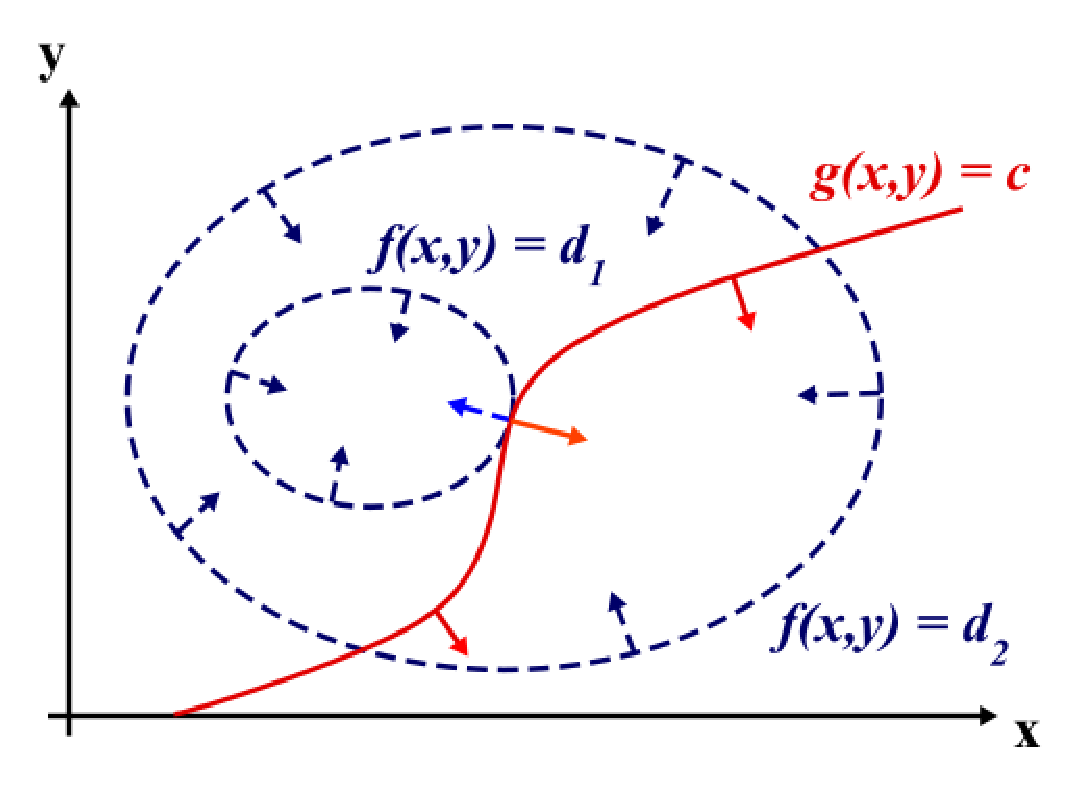
\epsfig{file=lagrange_multipliers.eps,width=\textwidth}
\caption[Illustration of Lagrange multiplier method]
{\label{fig:LagrangeMultipliers} \textit{Illustration of Lagrange Multiplier
    Method (credit Wikipedia) showing two contour lines of the objective
    function $f(x,y) = d_i$ (dark blue dashed lines) and the nonlinear
    constraint $g(x,y)=c$ (red solid line) as well as their gradients (blue
    and red arrows) at various positions including the constrained optimum
    (light blue and orange arrows).}
}
\end{figure}

The general nonlinear programming problem can be solved mathematically using
Lagrange's method. It assumes that the constraints cannot be used to
explicitly reduce the parameter space of the iteration variables - as it is
typically the case for non-linear constraints and objective functions - and is
therefore a powerful method applicable to a general class of problems.

If we assume for simplicity that we have a 2D problem with only one equality
constraint $c(x,y) = 0$, we know that we only need to search for the optimum
along that constraint. At the optimum, the value of the objective function
will then be stationary, i.e. it does not locally increase or decrease along
the constraint. As the gradient of a function is perpedicular to its contour
lines of $f(x,y) =d$, this is equivalent to saying that the gradient of the
objective function at that point is parallel to the gradient of the
constraints
\begin{equation}
\label{eqn:lagrangeequality}
\nabla f(x,y) = - \lambda \nabla c(x,y),
\end{equation}
where the factor $\lambda$ is necessary as only the direction, but not the
magnitude nor the sign of the gradients need to be equal. This is also
illustrated in Figure \ref{fig:LagrangeMultipliers}.

When expanding the method to several equality and inequality constraints we
can make use of the {\it Lagrange function}. For the nonlinear programming
problem described by \ref{eqn:NPP} it is given by
\begin{equation}
L(\vec{x},\vec{\lambda}) = f(\vec{x}) - \sum_{i=1}^{m} \lambda_i c_i(\vec{x}),
\end{equation}
with the corresponding {\it Lagrangian multipliers} $\lambda_i$. It allows us
to formulate the {\it first order necessary} conditions for a constrained
optimum $\vec{x}^*$ with corresponding Lagrange multipliers $\vec{\lambda}^*$,
the Karush-Kuhn-Tucker (KKT) conditions,
\begin{subequations}
\begin{align}
\nabla_x L(\vec{x}^*,\vec{\lambda}^*)  &= \nabla_x f(\vec{x}^*) - \sum_{i=1}^{m} \lambda_i \nabla_x c_i(\vec{x}^*) = 0,&&\\
\label{eqn:compl}
\lambda^*_i c_i(\vec{x}^*)       &= 0,                                             &i&=1,\dots,m,\\
c_i(\vec{x}^*)                   &= 0,                                             &i&=1,\dots,k,\\
\lambda^*_i                &\geq 0,                                          &i&=k+1,\dots,m,\\
c_i(\vec{x}^*)                   &\geq 0,                                         &i&=k+1,\dots,m.
\end{align}
\label{eqn:KKT}
\end{subequations}
Please note that by construction the Lagrange multipliers $\lambda_i^*$
fulfilling the KKT conditions are describing the derivative of the objective
function with respect to the constraint equation $\frac{df}{dc_i}$ and are
therefore a measure of how much the objective function changes with respect to
each constraint.

In the special case of a {\it continuously differentiable convex} objective
function $f(\vec{x})$ and equality constraints as well as {\it affine}
inequality constraints, these KKT conditions are also sufficient for a global
optimum. The \process\/ optimisation solver has been designed to converge on
the KKT conditions, but does not test whether these are {\it sufficient} for a
global optimum. It is therefore crucial that the user verifies that a global
optimum has been found.

Furthermore, these conditions and therefore the solver, assume that both the
objective function and constraints are at least {\it first order continuously
  partially differential}, i.e. that their first order partial derivatives are
all continuous functions. This might not always be the case in \process\/ and
is a potential source of errors.

\section{Sequential Quadratic Programming (SQP)}
\label{sec:SQP}
Based on the Lagrange method, sequential (also successive or recursive)
quadratic programming is the most efficient method to numerically solve
constrained nonlinear optimisation problems \cite{Schittkowski1980}. It
combines a simple solver for a quadratic optimisation problem with linear
constraints that determines a search direction $\vec{\delta}$ with a line
search to find an optimum along that search direction. It is a type of the
more general {\it feasible direction} methods which is itself a type of {\it
  primal method} that solve nonlinear programming problems in the $n-m$
dimensional feasible subspace \cite{Luenberger2008}.

% flow diagram of VMCON

\begin{figure}
\begin{centering}
\begin{tikzpicture}[scale=0.88,transform shape]
 
  %%%%%%%%%%%%%%%%%%%%%%%%%%%%%%%
  % Draw diagram elements

  %setup
  \path \boxwsubs {1}{Setup}{initialise $\mat{B}$\item evaluate $f$, $\vec{c}$, $\nabla_x f$, $\nabla_x \vec{c}$ \item j=0, \texttt{nfev}=1};

  %beginning of j-Iteration
  \path (p1.south)+(0.0,-1.5) \boxes{2}{Solve QSP, $j=j+1$};
  \path (p2.south)+(0.0,-1.) \boxes{3}{calculate $\vec{\lambda}^j$, $\nabla_x L$, $\vec{\mu}^j$, l = 1};
  \path (p3.south)+(0.0,-1.) \boxes{4}{test convergence};
 
  % Line search
  \path (p4.south)+(0.0,-1.5) \boxes{5}{Evaluate $\Phi(f,\vec{c})$};
  \path (p5.south)+(2.5,-1.5) \boxwsubs{6}{l == 1}{calculate $\Delta$ \item set $\alpha=1$};
  \path (p5.south)+(-2.5,-3.0) \boxwsubs{7}{l $>=$ 1}{test convergence \item calculate $\alpha$};
  \path (p7.south)+(2.5,-1.75) \boxes{8}{update $\vec{x}^j$, evaluate $f$, $\vec{c}$, \texttt{nfev} += 1, l += 1};

  %end of j-Iteration
  \path (p8.south)+(0.0,-1.25) \boxes{9}{evaluate $f$, $\vec{c}$, $\nabla_x f$, $\nabla_x \vec{c}$, calculate $\nabla_x L$ };
  \path (p9.south)+(0.0,-1.0) \boxes{10}{BFGS update};

  %%%%%%%%%%%%%%%%%%%%%%%%%%%%%%%
  % Draw arrows between elements

  %setup
  \path [line] (p1.south) -- node [above] {} (p2);
  \exit{p1}{0}

  %beginning of j-Iteration
  \path [line] (p2.south) -- node [above] {} (p3);
  \exithigher{p2}{5}
  \exitlower{p2}{6}
  \path [line] (p3.south) -- node [above] {} (p4);
  \path [line] (p4.south) -- node [above] {} (p5);
  \exitsucc{p4}{1}

  %Line search
  \path [line] (p5.south) -- +(0.0,-0.25) -- +(+2.5,-0.25)
  -- node [above, midway] {} (p6);
  \exitright{p6}{4}
  \path [line] (p5.south) -- +(0.0,-0.25) -- +(-2.5,-0.25)
  -- node [above, midway] {} (p7);
  \exitleft{p7}{3}
  \path [line] (p7.west)  |- +(-1.,-0.25)
  |- node [above, midway] {} (p9.west);

  %fix
  \path [linepart] (p7.west)  |- +(-1.,0.25)
  |- node [right, pos=0.4] {adhoc fix} (p2.west);

  \path [line] (p6.south) -- +(0.0,-0.5) |- +(-2.5,-1.9)
  -- node [above, midway] {} (p8);
  \path [line] (p7.south) -- +(0.0,-0.25) -- +(+2.5,-0.25)
  -- node [above, midway] {} (p8);
  \exit{p8}{2}
  \path [line] (p8.west)  |- +(-2.75,0.0)
  |- node [above, midway] {} (p5.west);

   %end of j-Iteration
  \path [line] (p9.south) -- node [above] {} (p10);
  \path [line] (p10.west)  |- +(-4.0,0.0)
  |- node [above, midway] {} (p2.west);

  %%%%%%%%%%%%%%%%%%%%%%%%%%%%%%%
  % Draw background boxes
 
  \outerbackground{p7}{p2}{p6}{p10}{SQP iteration}
  \mybackground{p7}{p5}{p6}{p8}{Line search}
  
\end{tikzpicture}
\caption[Flowchart of the \vmcon\ optimisation solver] { \textit{This is the
    flow chart of the \vmcon\/ optimisation solver. The criteria for and the
    interpretation of the successful (\ifail\/ = 1) and unsuccessful (\ifail\/
    $\neq$ 1) return parameters are described in Table \ref{tab:ifail}. }
\label{fig:vmconflow}
}
\end{centering}
\end{figure}

%%%%%%%%%%%%%%%%%%%%%%%%%%%%%%%%%%%%%%%%%%%
% VMCON return parameters

\begin{table}
\footnotesize
\begin{center}
\begin{tabular}{|c|p{2.7cm}|p{3.4cm}|p{3.4cm}|}
  \hline
  \ifail\/ & Description & Meaning & Recommendation \\
  \hline
  \colorbox{red!20}{ 0 }&\vmcon: Improper input parameters & The input
  parameters to the solver are wrong, e.g. negative number of iteration
  variables. & This needs to be fixed on the developer side and should only
  occur in the test phase of new modules. \\
  \hline
  \colorbox{green!20}{ 1 } &\vmcon: Normal return & \vmcon\/ has found a
  solution that fulfills the necessary conditions within the specified error
  tolerances (c.f. eq. \ref{eqn:vmcon_errtol}). & Test whether the solution is
  a global solution by using different starting parameters.\\
  \hline
  \colorbox{red!20}{ 2 } & Too many function calls & During the line search
  \vmcon\/ has reached the maximum number of total function calls
  (\texttt{maxfev}=100)  & \vmcon\/ struggles to find a solution. Retry with
  different start parameters. \\
  \hline
  \colorbox{red!20}{ 3 } & Line search required 10 functions calls & The
  results produced by input objective function/constraints and  their
  gradients are inconsistent. This can be due to numerical noise in the input
  functions. & The developer needs to check the consistency and numerical
  robustness of the objective function, constraints and their
  derivatives. Perhaps the accurracy in numerical
  integrations/differentiations needs to be higher. As a user, try changing
  the iteration bounds or adding other iteration variables. \\
  \hline
  \colorbox{red!20}{ 4 } & Uphill search direction was calculated & The
  quadratic subproblem has suggested a search direction in which the objective
  function only increases.  & This happens if an inconsistency between the
  objective function, the constraints and their respective derivatives occurs
  (c.f. \ifail\/ =3).\\
  \hline
  \colorbox{red!20}{ 5 }&\texttt{qpsub}: No feasible solution or bad
  approximation of Hessian & Either no optimum lies within the space allowed
  by the constraints and variable bounds or the identity matrix is not a good
  first approximation of the Hessian. & As a user, add a new iteration
  variable, as developer, try using a multiple of the identity matrix as
  initial Hessian instead.\\
  \hline
  \colorbox{red!20}{ 6 } &\texttt{qpsub}: Singular matrix in quadratic
  subproblem or restriction by artificial bounds & This is fairly
  self-explanatory. & If this is meaningful, widen the boundaries of the
  iteration variables.  \\
  \hline
  \colorbox{red!20}{ 7 } & Line search has been aborted & \Red{ADD SOME STUFF
    HERE (CHECK WITH MDK)} &   \\
  \hline
\end{tabular}
\end{center}
\caption{Summary of the description and  meaning of the \vmcon\/ return
  parameters \ifail\/. }
\label{tab:ifail}
\normalsize
\end{table}

\section{\vmcon}
\label{sec:vmcon}
The optimisation solver implemented in \process\/ is the Fortran routine
\vmcon\/ \cite{vmcon}. It is a modified version of the \texttt{vf02ad} routine
from the Harwell Software Library\footnote{www.hsl.rl.ac.uk} and implements a
SQP method originally suggested by Powell\footnote{This should not be confused
  with Powell's algorithm \cite{Powell1964} which solves a multidimensional
  unconstrained minimisation problem without derivatives.}~\cite{Powell1978}
based on work by Han \cite{Han1975}.  As stated before \vmcon\/ is designed to
converge on a solution of the {\it necessary} KKT conditions \ref{eqn:KKT}, but
does not check the {\it sufficient} conditions. Its convergence criterion is
therefore given by
\begin{equation}
\label{eqn:vmcon_errtol}
\left| \nabla_x f(\vec{x}^{j-1})^T \cdot \vec{\delta}^{j} \right| +
\sum^m_{i=1}\left| \lambda^j_i c_i(\vec{x}^{j-1}) \right| < \texttt{epsvmc}
\end{equation} %Yes, the j and j-1 are correct!
where \texttt{epsvmc} is a user specified error tolerance, $\vec{\delta}^j$ is
the vector in direction of the next line search (c.f. section
\ref{sec:linesearch}) and $j$ is the counter of the sequential quadratic
programming iteration. Hence, the first part estimates the predicted
improvement due to the next line search and the second part measures the error
in the complimentary condition \ref{eqn:compl} of the KKT conditions.

Figure \ref{fig:vmconflow} describes the flow chart of the \vmcon\/ routine,
while the various values of the return parameter \ifail\/\footnote{Note,
  within the \vmcon\/ routine \ifail\/ is called \texttt{info}.} are described
and interpreted in Table~\ref{tab:ifail}.

\section{The Quadratic Subproblem (QSP)}
\label{sec:QSP}
Within sequential quadratic programming the complex nonlinear problem is
broken down into solving a sequence of local quadratic subproblems with linear
constraints. This is based on the assumption that locally the problem is well
approximated by a second order Taylor expansion of the Lagrange
function. %Not the objective function!!!!
Hence, the local quadratic subproblem is described by
\begin{subequations}
\begin{align}
\textnormal{minimise } &Q(\vec{\delta}) = f(\vec{x}^{j-1}) + \vec{\delta}^T
\nabla_x f(\vec{x}^{j-1})+ \frac{1}{2} \vec{\delta}^T \nabla_{xx}
L(\vec{x}^{j-1},\vec{\lambda}^{j-1})\vec{\delta} \\
\textnormal{subject to } &\vec{\delta}^T \nabla_x c_i (\vec{x}^{j-1}) +
c_i(\vec{x}^{j-1}) = 0,\ i = 1,\dots,k,\\
\textnormal{and } &\vec{\delta}^T \nabla_x c_i (\vec{x}^{j-1}) +
c_i(\vec{x}^{j-1}) \geq 0,\ i = k+1,\dots,m,
\end{align}
\end{subequations}
where $\vec{\delta} = \vec{x} - \vec{x}^{j-1}$, the index $j-1$ indicates the
parameter values of the previous iteration\footnote{Note $j$ is called
  \texttt{nqp} in the \vmcon\/ routine.} and
$\nabla_{xx}L(\vec{x}^{j-1},\vec{\lambda}^{j-1})$ is the Hessian of the
Lagrange function. The solution of the QSP $\vec{\delta}$ describes the change
of the current iteration variable vector that minimises the local
approximation of the problem. To assure convergence even from bad starting
points, it is not directly used to update the iteration variable vector, but
describes the direction of the line search in which a 1d function is minimised
using a Newtonian method (c.f. section \ref{sec:linesearch}). Being a second
order approximation to the original problem, it typically has a faster
convergence that sequential linear programming (SLP) methods
\cite[chap. 10.4]{Bazaraa1993}.

To allow the applicability of the solver to more general problems, Powell
\cite{Powell1978} substituted the Hessian
$\nabla_{xx}L(\vec{x}^{j-1},\vec{\lambda}^{j-1})$ with a positive definite
approximation $\mat{B}$. This means that both the objective function
$f(\vec{x})$ and the constraint equations $c_i(\vec{x})$ only have to be
continuously differentiable instead of twice continuously differentiable with
respect to the iteration variable vector $\vec{x}$. This makes the method a
Quasi-Newtonian method as opposed to true Newtonian methods. How this
approximation is initialised and updated is described in more detail in the
section about the Broyden-Fletcher-Goldfarb-Shanno update \ref{sec:BFGS}.

To solve the QSP \vmcon\/ uses \texttt{harwqp} a modification of the the
Harwell library routine \texttt{VE02AD}, which in itself uses the subroutine
\texttt{harwfp/LA02AD} to find a feasible point within the variable bounds and
linearised constraints. Both routines go back to a method by Fletcher
\cite{Fletcher1970a,Fletcher1970b,Fletcher1970c}. The Lagrange multipliers are
also determined from results of the \texttt{harwqp} routine.

If the routine cannot find a feasible point it fails with \ifail\/ = 5
(c.f. Table \ref{tab:ifail}). As the routine is only checking the local linear
approximation of the constraints rather the full non-linear constraints, there
is a chance that a feasible point exists even though the routine fails with
\ifail\/ = 5. In these cases, it is possible that the first approximation of
the Hessian has not been good and the algorithm has, therefore, taken an
inappropriately large step. Then using a multiple of the identity matrix will
improve convergence of the algorithm.

If a singular matrix is encountered with the QSP solver or the solution is
restricted by the artificial bounds, \vmcon\/ fails with \ifail\/ = 6.  In
this case it can be helpful to widen the boundaries of the iteration
variables.

%XXX expand description of QSP routine??

\section{The Line Search}
\label{sec:linesearch}

The line search is an essential part of the SQP algorithm. As Powell
\cite{Powell1978} pointed out, it is necessary to allow convergence from poor
starting conditions. It uses the vector $\vec{\delta}$ from the QSP to update
$\vec{x}^j = \vec{x}^{j-1} + \alpha^j \vec{\delta}^j$ where the step-length
parameter $\alpha^j>0$ is determined by the line search as the parameter that
minimises
\begin{equation}
\Phi(\alpha) = f(\vec{x}) + \sum_{i=1}^k \mu_i \left| c_i(\vec{x})\right| +
\sum_{i=k+1}^m \mu_i \left| min(0,c_i(\vec{x}))\right|
\end{equation}
where the weights are defined as
\begin{equation}
\mu_i = 
\begin{cases}
|\lambda_i^1| & \textnormal{ if } j = 1,\\
max\left(|\lambda_i^j|,1/2(\mu_i^{j-1} + |\lambda_i^j|)\right) & \textnormal{ if } j > 1
\end{cases}
\end{equation}
to assure maximally efficient convergence \cite{Han1975}. Note, that in this
method locally {\it inactive} inequality constraints (c.f. \ref{sec:slack})
are not having any effect. It should always be possible, to find a solution
that fulfills
\begin{equation}
\Phi(\alpha=0)> \Phi(\alpha^j),
\end{equation}
if 
\begin{equation}
\left. \frac{d \Phi}{d\alpha}\right|_{\alpha=0} < 0.
\end{equation}
In case the derivative is positive (\texttt{dflsa} $\geq 0$), an uphill search
direction has been determined and the code stops with \ifail\/ =
4. %XXX(Though I don't think this dflsa is actually the true derivative!)
This typically only happens, if the objective function or constraints are
inconsistent with their own derivatives.

As the line search tries to determine the optimum of a one dimensional, but
fully non-linear function $\Phi(\alpha)$, it creates a series of $\alpha_l$
values\footnote{In the actual code $\alpha=$\texttt{calpha} and $\alpha_l
  =$\texttt{alpha}$*\alpha_{l-1}$.}. At each iteration $l$, a quadratic local
function $\Phi_l(\alpha)$ fullfilling the boundary conditions $\Phi_l(0) =
\Phi(0)$, $\Phi_l'(0)=\Delta$ and $\Phi_l(\alpha_{l-1}) = \Phi(\alpha_{l-1})$
is minimised, where typically
$\Delta=\Phi'(0)$. %XXX But I don't think this is the case in \vmcon (see comment above).
This leads to
\begin{equation}
\Phi_l(\alpha) = \Phi(0) + \Delta \alpha + \frac{\Phi(\alpha_{l-1})-\Phi(0) -
  \Delta \alpha_{l-1}}{\alpha_{l-1}^2} \alpha^2
\end{equation}
and minimising this gives 
\begin{equation}
\alpha_{min} = - \frac{\Delta\alpha_{l-1}^2}{2(\Phi(\alpha_{l-1})-\Phi(0) -
  \Delta \alpha_{l-1})}.
\end{equation}
Powell then sets $\alpha_l = \min(\alpha_{min}, 0.1\alpha_{l-1})$. On each
iteration the convergence of the line search is tested. It is reached, if
\begin{equation}
\Phi(\alpha_l) - \Phi(0) < 0.1 \Delta.
\end{equation}
which assures that the change in the function is small in comparison to its
derivative and 0.1 is a factor determined by experience. If this criterion is
successful, the code exits the line search and updates all function
evaluations.

As a modification to the original code, we have added an adhoc fix that exits
the line search in the case of
\begin{equation}
\Phi(\alpha_l) - \Phi(0) > 0.
\end{equation}
This has been added as experience have shown that \vmcon\/ typically does not
converge in these situations, but if it is forced to caculate a new search
direction in this way, it sometimes successfully finishes. Note, that this
cannot force \vmcon\/ to converge on any false solutions, as it only exits
positively when the convergence criterion \ref{eqn:vmcon_errtol} is fulfilled.

Typically, the line search already converges after one iteration and,
therefore, $\alpha = 1$. Hence, the \vmcon\/ line search has an upper limit of
maximally 10 iterations before it terminating with \ifail\/ = 3 (c.f. Table
\ref{tab:ifail}). This is higher than Powell's original limit of 5 to avoid a
few cases of early termination without a major effect on efficiency.

Within the line search \vmcon\/ also checks that the total number of function
calls has not exceeded \texttt{maxfev} = 100. If this is the case, it exits
with error code \ifail\/ = 2. Both checks assure that the routine stops, if it
does not seem to be able to find a solution.


\section{The Broyden-Fletcher-Goldfarb-Shanno (BFGS) quasi-Newton update}
\label{sec:BFGS}

\vmcon\/ uses a quasi-Newtonian update, the Broyden-Fletcher-Goldfarb-Shanno
update, in the approximation of the Hessian of the Lagrange function. This
means it is applicable to all continously differentialbe objective and
constraint functions. Note, that due to the constraints it is not actually
necessary for the Hessian of the solution to be positive definite, even though
this is essential for the convergence of the algorithm.

In quasi-Newtonian methods the identity matrix $\mat{I}$ is often chosen as an
initial estimate of the Hessian because of its positive definiteness. In some
cases it can be helpful to chose a constant multiple of the identity matrix
instead. The BGFS update \cite{Avriel2003} is one way of revising the initial
Hessian approximation using the update of the iteration variable vector
\begin{equation}
\vec{\xi} = \vec{x}^{j} - \vec{x}^{j-1}
\end{equation}
and the update of the Jacobian of the Lagrange function
\begin{equation}
\vec{\gamma} = \nabla_x L(\vec{x}^j,\vec{\lambda}^{j}) - \nabla_x
L(\vec{x}^{j-1},\vec{\lambda}^{j}). %NOT \lambda^{j-1}!!!
\end{equation}
Note that unless $\alpha=1$ in the line search, $\vec{\xi} \neq
\vec{\delta}$. To assure the positive definiteness of $\mat{B}$ Powell
\cite{Powell1978} suggested a variation of the standard formalism that uses
$\vec{\eta}$ instead of $\vec{\gamma}$
\begin{equation}
\vec{\eta} = \theta \vec{\gamma} + (1-\theta) \mat{B} \vec{\xi}
\end{equation}
with 
\begin{equation}
\theta = \left\{
\begin{array}{lr}
1 & \vec{\xi}^T \vec{\gamma} \geq 0.2 \vec{\xi}^T \mat{B} \vec{\xi} \\
\frac{0.8 \vec{\xi}^T B \vec{\xi}}{\vec{\xi}^T} & \vec{\xi}^T \vec{\gamma} <
0.2 \vec{\xi}^T \mat{B} \vec{\xi}
\end{array}
\right.
\end{equation}
to calculate a new approximation of the Hessian
\begin{equation}
\mat{B}_{new} = \mat{B} - \frac{\mat{B} \vec{\xi} \vec{\xi}^T
  \mat{B}}{\vec{\xi}^T \mat{B} \vec{\xi}}+\frac{\vec{\eta}^T
  \vec{\eta}}{\vec{\xi}^T \vec{\eta}}.
\end{equation}
Using the modified version of the BFGS update as suggested by Powell,
furthermore, assures superlinear convergence, even if the true Hessian is
indefinite \cite{Powell1977}.

\section{Symbols}
\label{sec:symbols}
In the previous sections the following conventions have been assumed:
$\vec{x}$, $\vec{\delta}$, $\vec{\xi}$, $\vec{\gamma}$ and $\vec{\eta}$ are
$n$-dimensional vectors, where $n$ is the number of iteration
variables. $\vec{c}$, $\vec{\lambda}$, $\vec{\mu}$ are $m$-dimensional
vectors, where $m$ is the total number of constraints and $c_i$, $\lambda_i$
and $\mu_i$ ($i=1\dots m$) are their respective components. $\mat{B}$ and
$\mat{I}$ are $n\times n$-dimensional matrices, while $\nabla_x \vec{c}$ is an
$n\times m$-dimensional matrix.

\bibliographystyle{unsrt}
\bibliography{Optimisation}

 %  The Optimisation Solver Explained
\myappendix{The Input File}
\label{app:infile}

The input file \indat\ is used to change the values of the physics,
engineering and other code parameters from their default values, and to set up
the numerics (constraint equations, iteration variables etc.) required to
define the problem to be solved.  The user interface writes the input file, so it is not necessary to edit it directly.

\subsection{Tokamak, stellarator, RFP or IFE?}
\label{sec:device}

The default model is the tokamak.  To select a stellarator, reversed field pinch or inertial fusion energy plant, an additional input file is required, \texttt{device.dat}, which should contain a single character in the first
line, which is interpreted as follows:
\begin{tabbing}
\hspace{15mm}\= \texttt{0} : use tokamak model \\
\> \texttt{1} : use stellarator model \\
\> \texttt{2} : use reversed field pinch model \\
\> \texttt{3} : use inertial fusion energy model
\end{tabbing}

\subsection{File format}

Variables can be specified in any order in the input file.  Comment lines start with a \texttt{*} character.  Data lines are of the form
\begin{verbatim}
variable = value
\end{verbatim}
where \texttt{variable} is the name of one of the input parameters or
iteration variables listed in the variable descriptor file, and \texttt{value}
is the (usually numerical) initial value required for that variable. (Arrays,
as opposed to scalar quantities, are treated differently --- see below.) All input data are screened for non-sensible values.

The following rules must be obeyed when writing an input file:

\begin{enumerate}

\item Each variable must be on a separate line.

\item Variable names can be upper case, lower case, or a mixture of both.

\item Spaces may not appear within a variable name or data value.

\item Other spaces within a line, and trailing spaces, are ignored.

\item Commas are not necessary between variables (but see below).

\item Data can extend over more than one line.

\item One-dimensional arrays can be explicitly subscripted, or unscripted, in
  which case the following element order is assumed: \texttt{A(1), A(2),
    A(3),...}

\item At present, multiple dimension arrays can only be handled without
  reference to explicit subscripts, in which case the following element order
  is assumed: \texttt{B(1,1), B(2,1), B(3,1),...} The use of the input file to
  specify multiple dimension array elements is prone to error.

\item Unscripted array elements must be separated by commas.

\item Blank lines are allowed anywhere in the input file.

\item Lines starting with a \texttt{*} are assumed to be comments.

\item Comment lines starting with five or more asterisks (i.e.\
  \texttt{*****}) are reproduced verbatim in the output file. This feature is not recommended, as these comments are likely to become out of date.  The user interface does not support this feature.

\item In-line comments are \textit{usually}\/ ignored, but there can be
  problems if one contains a comma (\texttt{,}). If this is the case, there
  must also be a comma after the variable's value and before the comment.

\end{enumerate}

It is useful to divide the input file into sections, using suitable comment
lines, to help the user keep related variables together.

The following is a valid fragment of an input file (the vertical lines are
simply to help show the column alignment):
\begin{center}
\begin{tabular}{||l}
$\!\!$\texttt{* This line is a comment that will not appear in the output} \\
$\!\!$\texttt{***** This line is a comment that will appear in the output} \\
$\!\!$\texttt{boundl(1) = 2.5,} \\
$\!\!$\texttt{BOUNDU(10) = 3.,} \\
$\!\!$\texttt{BOUNDU(45) = 1,} \\
$\!\!$\texttt{* Another comment... Note that real values can be entered as if} \\
$\!\!$\texttt{* they were integers, and vice versa (but it's not recommended...)} \\
$\!\!$\texttt{epsfcn = 10.e-4,} \\
$\!\!$\texttt{Ftol = 1.D-4,} \\
$\!\!$\texttt{* The next line sets the first five elements of array icc:} \\
$\!\!$\texttt{ICC =   2, 10, 11, 24, 31} \\
$\!\!$\texttt{* The next line sets the first ten elements of array ixc:} \\
$\!\!$\texttt{ixc =   10, 12, 3, 36, 48,} \\
$\!\!$\hspace{15mm}\texttt{1, 2, 6, 13, 16,} \\
$\!\!$\texttt{IOPTIMZ = 1,} \\
$\!\!$\texttt{maxcal = 200} \\
$\!\!$\texttt{ nsweep = 7} \\
$\!\!$\texttt{NEQNS = 5,    This is an in-line comment} \\
$\!\!$\texttt{NVAR = 10,    Another, but successfully containing a comma!} \\
\end{tabular}
\end{center}

The following are \textit{invalid}\/ entries in the input file
(Q: Why?!):
\begin{center}
\begin{tabular}{||l}
$\!\!$\texttt{boundl(1,1) = 2.5,} \\
$\!\!$\texttt{BOUNDU(N) = 3.,} \\
$\!\!$\texttt{A line of `random' characters like this will clearly wreak havoc} \\
$\!\!$\texttt{eps fcn = 10.e-4, ftol = 1.D-4} \\
$\!\!$\texttt{epsvmc = 1.0 e-4} \\
$\!\!$\texttt{ICC =   2  10  11  24  31} \\
$\!\!$\texttt{IOPTIMZ = 1.0,  This will in fact be okay - but is not recommended} \\
$\!\!$\texttt{NEQNS = 5    An in-line comment on a line with only one comma (,) character} \\
\end{tabular}
\end{center}

If the code encounters a problem reading the input file, it will stop immediately
with a (hopefully) useful error message. It may be worth looking at the
contents of the output file as well, to help narrow down on which line of the
input file the problem might lie.
\normalsize

 %  Non-optimisation Input File
\myappendix{Optimisation Input File}
\label{app:infile2}

The following is a typical input file used to run \process\ in optimisation
mode. Comments in [\ldots] have been added to the right of each line.

\footnotesize
\begin{verbatim}
* Numerics information                [Comment]

boundl(1) = 2.5,                      [Bound on iteration variable 1 (aspect)]
BOUNDU(10) = 3.,                      [Bound on iteration variable 10 (hfact)]
BOUNDU(60) = 4.d4,                    [Bound on iteration variable 60 (cpttf)]
NEQNS = 15,                           [Number of active constraint equations]
NVAR = 25                             [Number of active iteration variables]
ICC =   1,  2, 10, 11, 7, 16, 8, 24, 31, 32, 33, 34, 35, 36, 14, [Constraint eqns]
ixc =   5, 10, 12, 3,  7,        36, 48, 49, 50, 51, 53, 54, 19, [Corresponding...]
        1, 2, 4, 6, 13, 16, 29, 56, 57, 58, 59, 60,              [...iteration variables]
IOPTIMZ = 1,                          [Turn on optimisation]
MINMAX = 6,                           [Minimise cost of electricity]

ISWEEP=7,                             [Seven point scan]
NSWEEP=6,                             [Use WALALW as scanning variable]
SWEEP= 6.0,5.5,4.5,4.0,3.5,3.0,2.5    [Values of WALALW for each scan point]

* F-values and limits

FBETATRY = 1.0                        [N.B. active iteration variable 36]

* Physics parameters

ASPECT = 3.5,                         [N.B. active iteration variable 1]
BETA = 0.042,                         [N.B. active iteration variable 5]
BT = 6.,                              [N.B. active iteration variable 2]
DENE = 1.5e20,                        [N.B. active iteration variable 6]
FVSBRNNI = 1.0,                       [Non-inductive volt seconds fraction]
DNBETA = 3.5,                         [Beta g coefficient]
HFACT = 2.,                           [N.B. active iteration variable 10]
ICURR = 4,                            [Use ITER current scaling]
ISC = 6,                              [Use ITER 89-P confinement time scaling law]
IINVQD = 1,                           [Use inverse quadrature]
IITER = 1,                            [Use ITER fusion power calculations]
ISHAPE = 0,                           [Use input values for KAPPA and TRIANG]
KAPPA = 2.218,                        [Plasma elongation]
Q = 3.0,                              [Edge safety factor]
RMAJOR = 7.0,                         [N.B. active iteration variable 3]
RNBEAM = 0.0002,                      [N.B. active iteration variable 7]
TBURN = 227.9                         [Burn time]
TE = 15.,                             [N.B. active iteration variable 4]
TRIANG = 0.6                          [Plasma triangularity]

* Current drive parameters

IRFCD = 1,                            [Use current drive]
IEFRF = 5                             [Use ITER neutral beam current drive]
FEFFCD = 3.,                          [Artificially enhance efficiency]

* Divertor parameters

ANGINC=0.262,                         [Angle of incidence of field lines on plate]
PRN1=0.285                            [Density ratio]

* Machine build

BORE = 0.12,                          [N.B. active iteration variable 29]
OHCTH = 0.1,                          [N.B. active iteration variable 16]
GAPOH = 0.08,                         [Inboard gap]
TFCTH = 0.9,                          [N.B. active iteration variable 13]
DDWI = 0.07,                          [Vacuum vessel thickness]
SHLDITH = 0.69,                       [Inboard shield thickness]
BLNKITH = 0.115,                      [Inboard blanket thickness]
FWITH = 0.035,                        [Inboard first wall thickness]
SCRAPLI = 0.14,                       [Inboard scrape-off layer thickness]
SCRAPLO = 0.15,                       [Outboard scrape-off layer thickness]
FWOTH = 0.035,                        [Outboard first wall thickness]
BLNKOTH = 0.235,                      [Outboard blanket thickness]
SHLDOTH = 1.05,                       [Outboard shield thickness]
GAPOMIN = 0.21,                       [Outboard gap]
VGAPTF = 0,                           [Vertical gap]

* First wall, blanket, shield parameters

LBLNKT=0                              [Use old blanket model]
DENSTL=7800.                          [Steel density]

* TF coil parameters

OACDCP = 1.4e7,                       [N.B. active iteration variable 12]
ITFSUP = 1,                           [Use superconducting TF coils]
RIPMAX = 5.,                          [Maximum TF ripple]

* PF coil parameters

NGRP = 3,                             [Three groups of PF coils]
IPFLOC = 1,2,3,                       [Locations for each group]
NCLS = 2,2,2,1,                       [Number of coils in each group]
COHEOF = 1.85e7,                      [central solenoid current at End Of Flat-top]
FCOHBOP = 0.9,                        [central solenoid current at Begin. Of Pulse / COHEOF]
ROUTR = 1.5,                          [Radial position for group 3]
ZREF(3) = 2.5,                        [Z position for group 3]
OHHGHF = .71                          [Height ratio central solenoid / TF coil]

* Vacuum system parameters

NTYPE = 1                             [Use cryopump]

* Heat transport parameters

ETATH=0.35                            [Thermal to electric conversion efficiency]
FMGDMW = 0.                           [Power to MGF units]
BASEEL=5.e6                           [Base plant electric load]
ISCENR=2                              [Energy store option]

* Buildings

FNDT = 2.                             [Foundation thickness]
EFLOOR=1.d5                           [Effective total floor space]

* Costs

IREACTOR = 1,                         [Calculate cost of electricity]
IFUELTYP = 0                          [Treat blanket, first wall etc as capital cost]
UCHRS = 87.9,                         [Unit cost of heat rejection system]
UCCPCL1 = 250,                        [Unit cost of high strength tapered copper]
UCCPCLB = 150                         [Unit cost of TF outer leg plate coils]
\end{verbatim}
\normalsize

 %  Optimisation Input File
\myappendix{Source Code Documentation}
\label{app:doc}

The development of the \process\ code since its shipment from Oak Ridge
National Laboratory in April 1992 has been fully documented in the
Project Work File~\cite{PWF}. Presented here is a list of Project Work
File Notes as of \today\/ that address various issues related to the
source code.

\begin{itemize}
\item
Documentation of each individual source routine is an ongoing task. A
Work File Note will be produced as each routine is processed, with the
eventual aim of bringing all these together into a single document,
i.e.\ a future edition of this user guide.
\item
Summary of work performed since April 1992 : Note~0160
\item
Code status (routine SCCS version numbers) : Note~0165
\item
SCCS (Source Code Control System) implementation for \process: Note~0003
\item
Present code standard : Note~0160
\item
Future code standard (to be adhered to) : Note~0167
\item
Directory structure and location of all relevant files : Note~0168
\item
Proposed future work : Note~0160
\item
Pulsed power plant coding : Note~0189
\item
Nuclide inventory and activation (FISPACT) module : Notes~0195 and 0231
\item
New cost algorithms : Note~0224
\item
Stellarator model : Note~0246
\item
D-$^3$He tokamak model : Note~0265
\end{itemize}

Reference~\cite{PWF} has recently been superseded by a new Project Work File,
F/MI/PJK/PROCESS:-

\begin{itemize}
\item
Spherical Tokamak model: Note~001

\item
Reversed Field Pinch model: Note~009

\item
Test cases: Note~019

\end{itemize}

 %  Source Code Documentation

\end{document}
